\documentclass[UTF8,openany,zihao=-4,oneside]{ctexbook}

% Page and typography
\usepackage[a4paper,top=23mm,bottom=24mm,left=24mm,right=24mm,headheight=15pt,headsep=8mm,footskip=12mm]{geometry}
\linespread{1.08}
\raggedbottom
\sloppy
\emergencystretch=3em

% Core packages
\usepackage{amsmath,amssymb,mathtools}
\usepackage{graphicx}
\usepackage{booktabs,longtable,array,tabularx,multirow,makecell}
\usepackage{enumitem}
\usepackage[table]{xcolor}
\usepackage{tikz}
\usetikzlibrary{positioning,arrows.meta,calc,fit,shapes.geometric}
\usepackage{caption}
\usepackage{float}
\usepackage{fancyhdr}
\usepackage{titlesec}
\usepackage{titletoc}
\usepackage{tocloft}
\usepackage[most]{tcolorbox}
\usepackage{listings}
\usepackage{etoolbox}
\usepackage{hyperref}
\usepackage{bookmark}

% Brand colors
\definecolor{FGBlue}{HTML}{1F4E79}
\definecolor{FGDeep}{HTML}{102A43}
\definecolor{FGCyan}{HTML}{2E8BC0}
\definecolor{FGOrange}{HTML}{D98A15}
\definecolor{FGGray}{HTML}{F3F6F9}
\definecolor{FGLine}{HTML}{D7E2EA}
\definecolor{FGText}{HTML}{243B53}

\hypersetup{
  colorlinks=true,
  linkcolor=FGBlue,
  urlcolor=FGCyan,
  citecolor=FGOrange,
  pdfauthor={FlameGuard},
  pdftitle={稳燃宝控制器技术手册},
  pdfsubject={模型预测控制、控制接口、状态估计与安全边界},
  pdfkeywords={FlameGuard, 稳燃宝, 控制器, 模型预测控制, MPC, 技术手册}
}

% Paragraph and list tuning
\setlength{\parindent}{2em}
\setlength{\parskip}{0.18em}
\setlist{itemsep=0.15em,topsep=0.35em,leftmargin=2.2em}
\renewcommand{\arraystretch}{1.22}
\setlength{\tabcolsep}{5pt}
\setlength{\LTleft}{0pt}
\setlength{\LTright}{0pt}
\AtBeginEnvironment{longtable}{\small\renewcommand{\arraystretch}{1.2}}

% Pandoc compatibility
\providecommand{\tightlist}{\setlength{\itemsep}{0pt}\setlength{\parskip}{0pt}}
\providecommand{\passthrough}[1]{#1}
\newcommand{\manualdivider}{\par\vspace{0.6em}\noindent\textcolor{FGLine}{\rule{\linewidth}{0.7pt}}\vspace{0.6em}\par}

% Captions
\captionsetup{font=small,labelfont={bf,color=FGBlue},labelsep=quad}

% Chapter / section styles
\titleformat{\chapter}[display]
  {\Huge\bfseries\sffamily\color{FGDeep}}
  {\begin{tikzpicture}[baseline=(n.base)]\node[fill=FGBlue,text=white,rounded corners=1.5mm,inner xsep=8pt,inner ysep=5pt,font=\Large\bfseries\sffamily] (n) {第\thechapter 章};\end{tikzpicture}}
  {0.85em}
  {\Huge}
  [\vspace{0.35em}{\color{FGOrange}\titlerule[1.2pt]}]
\titlespacing*{\chapter}{0pt}{-4mm}{11mm}

\titleformat{\section}
  {\Large\bfseries\sffamily\color{FGBlue}}
  {\thesection}{0.75em}{}
  [\vspace{0.15em}{\color{FGLine}\titlerule[0.6pt]}]
\titlespacing*{\section}{0pt}{2.1ex plus .4ex}{1.1ex}

\titleformat{\subsection}
  {\large\bfseries\sffamily\color{FGDeep}}
  {\thesubsection}{0.75em}{}
\titlespacing*{\subsection}{0pt}{1.8ex plus .3ex}{0.8ex}

\titleformat{\subsubsection}
  {\normalsize\bfseries\sffamily\color{FGDeep}}
  {\thesubsubsection}{0.65em}{}
\titlespacing*{\subsubsection}{0pt}{1.3ex plus .2ex}{0.55ex}

% TOC styling
\renewcommand{\cftchapfont}{\sffamily\bfseries\color{FGDeep}}
\renewcommand{\cftsecfont}{\sffamily\color{FGText}}
\renewcommand{\cftchappagefont}{\sffamily\bfseries\color{FGBlue}}
\renewcommand{\cftsecpagefont}{\sffamily\color{FGText}}
\setlength{\cftbeforechapskip}{0.45em}

% Header / footer
\pagestyle{fancy}
\fancyhf{}
\fancyhead[L]{\sffamily\small\color{FGDeep}“稳燃宝”控制器技术手册}
\fancyhead[R]{\sffamily\small\color{FGBlue}\leftmark}
\fancyfoot[L]{\sffamily\scriptsize\color{FGText}控制设计 · 接口约定 · 模型预测控制}
\fancyfoot[R]{\sffamily\small\bfseries\color{FGBlue}\thepage}
\renewcommand{\headrulewidth}{0.5pt}
\renewcommand{\footrulewidth}{0pt}
\renewcommand{\headrule}{\hbox to\headwidth{\color{FGLine}\leaders\hrule height \headrulewidth\hfill}}
\fancypagestyle{plain}{%
  \fancyhf{}%
  \fancyfoot[R]{\sffamily\small\bfseries\color{FGBlue}\thepage}%
  \renewcommand{\headrulewidth}{0pt}%
}

% Code listings
\lstdefinestyle{fgcode}{
  basicstyle=\ttfamily\small,
  backgroundcolor=\color{FGGray},
  frame=single,
  rulecolor=\color{FGLine},
  framerule=0.5pt,
  breaklines=true,
  columns=fullflexible,
  keepspaces=true,
  showstringspaces=false,
  tabsize=2,
  xleftmargin=1em,
  xrightmargin=1em,
  framexleftmargin=0.6em,
  framexrightmargin=0.6em,
  aboveskip=0.8em,
  belowskip=0.8em
}
\lstset{style=fgcode}

% Inline code and quotes
\newcommand{\fgbadge}[1]{\tcbox[colback=FGBlue!6,colframe=FGBlue!35,boxrule=0.4pt,arc=1mm,left=2pt,right=2pt,top=1pt,bottom=1pt,on line]{\sffamily\footnotesize #1}}

\begin{document}

% Cover
\begin{titlepage}
\begin{tikzpicture}[remember picture,overlay]
  \fill[FGDeep] (current page.north west) rectangle ([yshift=-88mm]current page.north east);
  \fill[FGBlue] ([yshift=-88mm]current page.north west) rectangle ([yshift=-92mm]current page.north east);
  \fill[FGOrange] ([yshift=-92mm]current page.north west) rectangle ([yshift=-94mm]current page.north east);
  \fill[FGGray] ([yshift=-94mm]current page.north west) rectangle (current page.south east);
  \draw[FGBlue!20,line width=1.2pt] ([xshift=18mm,yshift=-122mm]current page.north west) -- ([xshift=-18mm,yshift=-122mm]current page.north east);
\end{tikzpicture}
\vspace*{13mm}
{\sffamily\bfseries\color{white}\fontsize{18}{22}\selectfont FlameGuard / 稳燃宝}\par
\vspace{9mm}
{\sffamily\bfseries\color{white}\fontsize{34}{42}\selectfont 控制器技术手册}\par
\vspace{4mm}
{\sffamily\color{white}\fontsize{15}{20}\selectfont 控制设计 · 变量接口 · 模型预测控制 · 安全边界}\par
\vspace{36mm}
\begin{tcolorbox}[enhanced,width=\textwidth,colback=white,colframe=FGLine,boxrule=0.7pt,arc=2mm,drop shadow={black!12!white},left=8mm,right=8mm,top=6mm,bottom=6mm]
{\sffamily\bfseries\Large\color{FGDeep}v0.2.0 Beta}\par\vspace{0.6em}
\end{tcolorbox}
\vfill
{\sffamily\small\color{FGText}炉火纯青队 · 大学生节能减排社会实践与科技竞赛 · 2025}\par
\end{titlepage}

\frontmatter
\pagestyle{plain}
\tableofcontents
\cleardoublepage
\pagestyle{fancy}
\mainmatter

\chapter{概述}\label{chap:overview}

\section{控制器的工程定位}\label{sec:controller-position}

“稳燃宝”（FlameGuard）控制器是连接垃圾预热炉、主焚烧炉、现场观测系统和执行机构的控制决策单元。对于小型垃圾焚烧厂或乡镇级生活垃圾处理场景，来料组分和含水率通常波动较大，焚烧炉本身热惯性有限，炉膛温度容易受到高含水率垃圾的冲击。控制器的工程任务，是在垃圾进入主焚烧炉之前，通过调节预热炉的换热侧烟气温度和循环速度，使未来进入焚烧炉的物料状态更加有利于稳定燃烧。

从系统位置看，控制器位于“观测--估计--预测--决策--执行”的中间层。上游输入来自现场或仿真对象的观测数据，包括预热炉出口状态、焚烧炉平均温度、烟囱温度、烟囱速度、执行器反馈和设备健康状态等。下游输出为预热炉侧的热风温度参考、循环速度参考以及经执行层处理后的温度和速度命令。换言之，控制器通过预热炉影响垃圾含水率和固体温度，再由改变后的物料状态影响焚烧炉的燃烧结果。

这种控制关系决定了“稳燃宝”控制器具有明显的前馈预测和慢动态调节特征。若主焚烧炉当前平均温度已经下降，当前投入预热炉的控制动作并不会立刻改变炉膛温度。预热炉内部物料需要经历轴向输运、升温、蒸发和出口排出，进入焚烧炉后还要经过燃烧响应和烟气状态变化。控制器必须在这些滞后和惯性存在的条件下提前判断未来趋势，而不能只对当前温度误差进行瞬时修正。

图 \ref{fig:controller-position} 给出了控制器在稳燃宝系统中的位置。图中实线表示物料或热资源流向，虚线表示信息反馈和控制命令流向。预热炉和焚烧炉构成被控对象的主要物理部分，控制器则根据观测量和预测模型生成预热炉工况命令。

\begin{figure}[htbp]
  \centering
  \begin{tikzpicture}[
    node distance=10mm and 12mm,
    box/.style={
      draw=FGBlue,
      fill=FGBlue!6,
      very thick,
      rounded corners=2mm,
      minimum height=12mm,
      text width=30mm,
      align=center,
      font=\sffamily\small
    },
    orangebox/.style={
      draw=FGOrange,
      fill=FGOrange!9,
      very thick,
      rounded corners=2mm,
      minimum height=12mm,
      text width=38mm,
      align=center,
      font=\sffamily\small
    },
    graybox/.style={
      draw=FGLine,
      fill=FGGray,
      thick,
      rounded corners=2mm,
      minimum height=10mm,
      text width=28mm,
      align=center,
      font=\sffamily\small
    },
    arrow/.style={
      -{Latex[length=2.8mm,width=2mm]},
      very thick,
      FGBlue!80
    },
    cArrow/.style={
      -{Latex[length=2.8mm,width=2mm]},
      very thick,
      FGOrange!85,
      dashed
    }
  ]
  
  % 顶部工程主流程
  \node[graybox] (feed) {入口垃圾\\含水率/流量};
  \node[box, right=of feed] (pre) {垃圾预热炉\\升温与脱水};
  \node[box, right=of pre] (furnace) {主焚烧炉\\燃烧响应};
  \node[graybox, right=of furnace] (stack) {烟囱/烟气\\资源边界};
  
  % 底部闭环模块
  \node[orangebox, below=22mm of pre] (ctrl) {稳燃宝控制器\\预测、优化、执行保护};
  \node[graybox, below=22mm of furnace] (obs) {观测与估计\\温度/速度/状态};
  
  % 物料与烟气主流程
  \draw[arrow] (feed) -- (pre);
  \draw[arrow] (pre) -- node[above, font=\scriptsize\sffamily] {$\omega, T$} (furnace);
  \draw[arrow] (furnace) -- node[above, font=\scriptsize\sffamily] {$T, v$} (stack);
  
  % 观测链路：主焚烧炉与烟气资源均进入观测与估计
  \draw[cArrow] (furnace.south) -- 
    node[right, font=\scriptsize\sffamily] {燃烧状态} 
    (obs.north);
  
  \draw[cArrow] (stack.south) -- 
    (obs.east);
  
  % 控制器接收估计状态，并向预热炉下发控制作用
  \draw[cArrow] (obs.west) -- 
    node[below, font=\scriptsize\sffamily] {}
    (ctrl.east);
  
  \draw[cArrow] (ctrl.north) -- 
    node[right, font=\scriptsize\sffamily] {$T, v$}
    (pre.south);
  
  \end{tikzpicture}
  \caption{控制器在“稳燃宝”系统中的工程位置}
  \label{fig:controller-position}
\end{figure}

\manualdivider

\section{控制因果链}\label{sec:direct-and-indirect-control}

稳燃宝控制器的直接调节对象是预热炉换热侧工况。当前设计中，控制器主要调节两个连续变量：热风温度 \(T_g\) 和换热侧气流速度 \(v_g\)。热风温度决定进入预热炉换热通道的烟气或补热烟气的热位，气流速度决定换热侧对流换热能力、烟气质量流量需求和风机/循环系统负荷。二者共同决定预热炉对垃圾的升温和脱水能力。

但是，控制器真正关心的最终结果并不是 \(T_g\) 或 \(v_g\) 本身，而是主焚烧炉燃烧状态的稳定性。预热炉出口垃圾湿基含水率 \(\omega_{out}\) 和出口垃圾等效固体温度 \(T_{s,out}\) 是连接直接调节对象与最终燃烧状态的中间变量。一般而言，在进料量和热值近似相同的情况下，进入焚烧炉的垃圾含水率越高，水分蒸发消耗的热量越大，主燃烧区平均温度越容易下降；进入焚烧炉的垃圾含水率越低，焚烧炉用于水分蒸发的热负荷越小，炉温越容易维持在稳定区间。

因此，本控制器的控制因果链可以写成：

\[
\left(T_{g,ref},v_{g,ref}\right)
\longrightarrow
\left(T_{g,cmd},v_{g,cmd}\right)
\longrightarrow
\left(\omega_{out},T_{s,out}\right)
\longrightarrow
\left(\omega_b,r_d\right)
\longrightarrow
\left(T_{avg},T_{stack},v_{stack}\right)
\]

其中，\(T_{g,ref}\) 和 \(v_{g,ref}\) 是控制器决策层给出的参考值；\(T_{g,cmd}\) 和 \(v_{g,cmd}\) 是执行层经过限幅、限速、一阶动态、补热和辅助循环诊断之后真正下发的命令；\(\omega_{out}\) 是预热炉出口垃圾含水率；\(\omega_b\) 是进入焚烧炉并参与燃烧响应的等效含水率；\(r_d\) 是进入焚烧炉的干基质量流率相对于基准干基流率的无量纲比值；\(T_{avg}\)、\(T_{stack}\) 和 \(v_{stack}\) 分别表示焚烧炉平均温度、烟囱温度和烟囱速度。

\manualdivider

\section{控制目标}\label{sec:control-objectives}

稳燃宝控制器的目标可分为主控制目标、过程质量目标、执行约束目标、资源经济性目标和异常工况目标。

\subsection{主控制目标}\label{subsec:main-objective}

主控制目标是维持主焚烧炉燃烧稳定，尤其是保持焚烧炉平均温度 \(T_{avg}\) 不低于安全与合规要求，并尽量运行在目标参考区间内。在当前设计中，焚烧炉平均温度的关键下限为：

\[
T_{avg}\geq 850^\circ\mathrm{C}
\]

该温度下限为保证垃圾燃烧废气中二噁英充分分解的必须温度，也是国家标准要求的焚烧炉燃烧区域最低温度下限。与普通跟踪误差相比，低温风险更接近安全约束，因此其处理权重应高于一般经济性目标。

\subsection{执行约束目标}\label{subsec:actuation-constraint-objective}

执行约束目标用于保证控制器输出可被真实执行机构接受。对于热风温度通道，控制器必须考虑温度上限、温度下限、升降温速率和热源能力。对于气流速度通道，控制器必须考虑风机、阀门、管道和循环系统允许的速度范围以及速度变化率。当前设计中，参考层通常在较保守的温度范围内优化，而执行层保留更大的安全恢复余量。

执行约束可以分为硬约束和软约束。硬约束通常对应设备物理边界，例如热风温度不能低于最小可用温度，气流速度不能超过风机和管路允许上限。软约束通常对应控制性能和运行偏好，例如尽量减少高风速运行、尽量降低补热功率、尽量避免温度低于参考区间。对于硬约束，控制器不应通过优化权重来“折中突破”；对于软约束，控制器可以在安全和经济性之间进行权衡。

\subsection{资源经济性目标}\label{subsec:economy-objective}

稳燃宝控制器不应把所有资源都视为无限可用。预热炉热风温度可能由自然烟气资源和辅助补热共同形成，预热炉气流速度可能由自然烟气抽取和辅助循环共同满足。若控制器长期要求高 \(T_g\) 和高 \(v_g\)，系统可能能够维持较高炉温，但代价是补热功率、辅助循环流量和风机功率显著增加。因此，资源经济性目标是控制器设计中不可缺少的一部分。

资源经济性目标并不等于禁止补热或禁止辅助循环。对于突发低温和高含水率来料冲击，辅助补热和高循环速度可能是必要的安全恢复手段。稳燃宝的设计中，正常参考区间内尽量经济运行，接近或低于安全边界时优先恢复炉温。也就是说，经济性目标在不同运行状态下权重不同。当炉温处于安全参考区间内时，高风速、高补热和辅助循环应受到较强惩罚；当炉温接近合规下限时，安全恢复应优先于经济性。

\subsection{异常工况目标}\label{subsec:abnormal-objective}

异常工况目标用于处理模型预测不可行、优化失败、观测异常、通信延迟、执行器反馈异常或焚烧炉温度已经低于安全下限等情况。在这些情况下，控制器不能继续只依赖正常优化结果。它需要具备降级运行、保持上次可信命令、触发安全恢复、提高重优化频率或请求现场上层系统介入的能力。

异常工况目标的核心是保证系统有清晰的行为边界。例如，当测得 \(T_{avg}<850^\circ\mathrm{C}\) 时，控制器应进入更积极的恢复策略；当优化器无法在规定时间内找到可接受解时，应使用保守的 fallback 参考；当执行器反馈显示命令未被真正执行时，状态估计应降低置信度并避免盲目信任模型预测。异常工况控制必须与现场硬件联锁和人工干预机制相互配合，不能把软件恢复策略误写成最终安全保护。

\manualdivider

\section{闭环链路}\label{sec:closed-loop}

稳燃宝控制器采用闭环控制结构。控制器在每个控制周期根据最新观测更新对系统状态的理解，并据此重新计算控制动作。闭环链路包括状态观测、状态估计、未来预测、控制决策、命令执行和反馈校正六个环节。

状态观测环节从被控对象获得当前观测快照。该快照至少应包括焚烧炉平均温度、烟囱温度和烟囱速度。在仿真环境或高配置现场系统中，还可能包括完整预热炉轴向状态、预热炉出口含水率、出口固体温度、执行器实际状态、烟气资源测量和设备健康状态。观测环节的质量直接影响控制器后续判断。如果观测量缺失或延迟，控制器必须通过状态估计和置信度处理来补偿。

状态估计环节把现场观测转化为控制器内部可用状态。对于预热炉，真实设备未必能够直接提供全部轴向槽段状态，因此估计器需要在“有完整状态观测”和“只有有限出口观测”两类情况下均能工作。当完整预热炉状态可用时，控制器可以直接同步内部预测模型；当完整状态不可用时，控制器需要根据上一时刻命令、入口垃圾观测和预热炉预测模型推进一个控制器侧数字孪生，并用出口含水率或出口温度等有限观测进行校正。

未来预测环节利用预热炉和焚烧炉模型，模拟候选控制动作在未来一段时间内可能造成的影响。预测过程不是只预测 \(T_{avg}\)，而是同时预测出口含水率、入炉含水率、干基流率比、烟囱温度、烟囱速度、补热需求、辅助循环需求和风机功率等。只有这样，控制器才能判断某个动作虽然能提高炉温，但是否会造成过高资源消耗或执行压力。

控制决策环节根据预测结果选择最优控制参考。当前设计采用模型预测控制思想，即在有限预测时域内比较不同 \(T_g\)、\(v_g\) 序列的未来结果，并在温度、含水率、约束、能耗和安全风险之间进行权衡。决策层输出参考值 \(T_{g,ref}\)、\(v_{g,ref}\)。

命令执行环节将参考值转化为实际命令 \(T_{g,cmd}\)、\(v_{g,cmd}\)。执行层必须施加温度和速度限幅、变化率限制、一阶执行器动态、补热计算、辅助循环诊断和安全恢复逻辑。这样处理的原因是，优化器给出的参考值代表控制意图，但现场设备只能按照自身动态和安全边界执行。

反馈校正环节在下一控制周期发生。控制器将实际观测到的炉温、烟气状态和执行器反馈与模型预测相比较，估计模型偏差和外部扰动，并更新下一次优化。正是这一环节使系统能够抵抗来料扰动、模型误差和现场资源变化。

该闭环链路具有两个重要特点。第一，它是慢变量闭环。控制器的动作通过预热炉和物料输运影响未来焚烧炉状态，而不是立即改变当前炉温。第二，它是模型参与的闭环。控制器不仅使用当前测量值，还使用内部预测模型评估未来结果。因此，控制器的性能取决于观测、估计、预测和执行四个部分共同作用，不能单独归因于某一个优化器。

\manualdivider

\section{安全边界与责任边界}\label{sec:safety-boundary}

稳燃宝控制器可以降低焚烧炉低温、不稳定燃烧和资源浪费的概率，但它不是现场硬件安全联锁系统，也不能替代燃烧保护系统、急停系统、超温保护、风机保护、烟气排放安全系统或人工值守制度。

本控制器的安全边界可以分为四层。第一层是优化层安全边界。MPC 在求解未来控制动作时，会将热风温度、循环速度、炉膛温度安全区间、补热和辅助循环代价纳入考虑。该层的作用是尽量在正常预测范围内避免系统进入危险区域。第二层是执行层安全边界。执行层对参考值施加限幅、限速和一阶动态，并在必要时记录补热、辅助循环和风机功率需求。第三层是软件恢复层安全边界。当炉温已经低于安全下限，或预测显示常规优化难以及时恢复时，控制器可以请求安全恢复，执行层将温度和速度参考提升到恢复策略所要求的水平。第四层是现场硬件安全边界。它包括电气联锁、机械保护、燃烧安全、超温保护、烟气处理系统保护和人工紧急干预。

表 \ref{tab:safety-layer} 给出了四层安全边界的职责划分。

\begin{longtable}{@{}p{0.18\linewidth}p{0.32\linewidth}p{0.39\linewidth}@{}}
\caption{控制器相关安全层级与责任边界}\label{tab:safety-layer}\\
\toprule
层级 & 主要对象 & 责任说明 \\
\midrule
\endfirsthead
\toprule
层级 & 主要对象 & 责任说明 \\
\midrule
\endhead
优化层 & MPC 目标函数与约束 & 在预测时域内权衡炉温、含水率、能耗和动作平滑性；尽量避免未来状态跌破安全边界，但受模型准确性和扰动可预测性限制。 \\
执行层 & 命令转换与执行器动态 & 将参考值转化为可执行命令，施加限幅、限速、一阶滞后、补热和辅助循环诊断；防止参考值被直接当成现场命令。 \\
软件恢复层 & recovery guard / fallback & 在低温、预测不可行或优化失败时触发保守恢复动作；该层强调及时恢复，不追求经济最优。 \\
现场硬件层 & PLC、联锁、急停和保护系统 & 承担最终安全保护职责；控制器不得替代现场强制安全联锁和人工处置机制。 \\
\bottomrule
\end{longtable}

从责任边界看，控制器可以做三件事：第一，根据当前观测和预测模型给出合理的预热炉工况；第二，在命令下发前执行软件层保护；第三，在异常状态下进入安全恢复或降级控制。但控制器不能保证所有传感器永远正确，不能保证执行机构一定按命令动作，不能保证模型覆盖全部极端扰动，也不能替代现场法规和硬件保护要求。因此，在正式工程部署中，控制器应被视为运行优化和燃烧稳定性增强系统，而不是唯一安全保障系统。

\manualdivider

\chapter{变量名与接口约定}\label{chap:variables-interfaces}

\section{变量命名原则}\label{sec:naming-principles}

控制器变量命名遵循“物理量主体 + 状态后缀 + 单位后缀”的原则。

状态后缀用于说明同一物理量处于闭环链路中的哪个位置。常用后缀如表 \ref{tab:suffix} 所示。

\begin{longtable}{@{}p{0.18\linewidth}p{0.28\linewidth}p{0.44\linewidth}@{}}
\caption{控制器变量状态后缀约定}\label{tab:suffix}\\
\toprule
后缀 & 含义 & 使用说明 \\
\midrule
\endfirsthead
\toprule
后缀 & 含义 & 使用说明 \\
\midrule
\endhead
\(ref\) & 参考值 & 由控制决策层输出，表示希望系统达到的目标或控制意图，例如 \(T_{g,ref}\)、\(v_{g,ref}\)。 \\
\(cmd\) & 命令值 & 经执行层限幅、限速、一阶动态和安全保护后真正下发给 plant 或现场执行机构的值，例如 \(T_{g,cmd}\)、\(v_{g,cmd}\)。 \\
\(meas\) & 测量值 & 来自传感器或现场观测系统的值。若测量信号经过滤波或同步，应在接口说明中明确。 \\
\(est\) & 估计值 & 由状态估计器根据观测、模型和历史命令推断得到的值，常用于不可直接测量的内部状态。 \\
\(pred\) & 预测值 & 由预测模型在未来时域内计算得到的值，用于 MPC 评价候选控制动作。 \\
\(target\) & 目标值 & 表示控制目标或动态设定目标，可能由上层设定，也可能由控制器根据炉温目标反推得到。 \\
\bottomrule
\end{longtable}

在数学公式中，单位通常由符号表统一说明。在代码字段和接口字段中，在字段名后附加单位后缀，以避免不同单位制混用。例如：

\begin{lstlisting}
Tg_ref_C
Tg_cmd_C
vg_ref_mps
vg_cmd_mps
T_avg_C
T_stack_C
v_stack_mps
Q_aux_heat_kW
mdot_aux_flow_kgps
\end{lstlisting}

其中，\texttt{\_C} 表示摄氏度，\texttt{\_mps} 表示米每秒，\texttt{\_kgps} 表示千克每秒，\texttt{\_kW} 表示千瓦。对于无量纲变量，例如湿基含水率 \(\omega\) 和干基质量流率比 \(r_d\)，代码字段可以不加单位后缀，但应在接口说明中明确其取值范围和含义。

数学符号和代码字段一一对应。表 \ref{tab:math-code-map} 给出了常用变量的对应关系。

\begin{longtable}{@{}p{0.17\linewidth}p{0.23\linewidth}p{0.18\linewidth}p{0.32\linewidth}@{}}
\caption{主要数学符号与工程字段对应关系}\label{tab:math-code-map}\\
\toprule
数学符号 & 推荐字段名 & 单位 & 说明 \\
\midrule
\endfirsthead
\toprule
数学符号 & 推荐字段名 & 单位 & 说明 \\
\midrule
\endhead
\(T_{g,ref}\) & \texttt{Tg\_ref\_C} & \(^\circ\mathrm{C}\) & 控制器输出的热风温度参考。 \\
\(T_{g,cmd}\) & \texttt{Tg\_cmd\_C} & \(^\circ\mathrm{C}\) & 执行层输出的热风温度命令。 \\
\(v_{g,ref}\) & \texttt{vg\_ref\_mps} & \(\mathrm{m/s}\) & 控制器输出的气流速度参考。 \\
\(v_{g,cmd}\) & \texttt{vg\_cmd\_mps} & \(\mathrm{m/s}\) & 执行层输出的气流速度命令。 \\
\(\omega_{out}\) & \texttt{omega\_out} & -- & 预热炉出口湿基含水率，小数形式。 \\
\(\omega_b\) & \texttt{omega\_b} & -- & 进入焚烧炉的等效湿基含水率，小数形式。 \\
\(r_d\) & \texttt{rd} & -- & 焚烧炉干基质量流率比。 \\
\(T_{avg}\) & \texttt{T\_avg\_C} & \(^\circ\mathrm{C}\) & 焚烧炉平均温度。 \\
\(T_{stack}\) & \texttt{T\_stack\_C} & \(^\circ\mathrm{C}\) & 烟囱温度或可用烟气温度。 \\
\(v_{stack}\) & \texttt{v\_stack\_mps} & \(\mathrm{m/s}\) & 烟囱出口速度。 \\
\(Q_{aux}\) & \texttt{Q\_aux\_heat\_kW} & \(\mathrm{kW}\) & 辅助补热需求。 \\
\(\dot m_{aux}\) & \texttt{mdot\_aux\_flow\_kgps} & \(\mathrm{kg/s}\) & 辅助循环或补偿流量需求。 \\
\bottomrule
\end{longtable}

\manualdivider

\section{控制变量与执行命令}\label{sec:control-and-command-vars}

\subsection{热风温度变量族}\label{subsec:Tg-family}

热风温度变量族以 \(T_g\) 为主体，用于描述进入预热炉换热侧的等效烟气温度或补热后热风温度。控制器中至少需要区分以下变量：

\begin{longtable}{@{}p{0.18\linewidth}p{0.24\linewidth}p{0.48\linewidth}@{}}
\caption{热风温度变量族}\label{tab:Tg-family}\\
\toprule
变量 & 工程含义 & 说明 \\
\midrule
\endfirsthead
\toprule
变量 & 工程含义 & 说明 \\
\midrule
\endhead
\(T_{g,ref}\) & 热风温度参考值 & 由 MPC 或 fallback 决策层输出，表示当前控制周期希望预热炉换热侧达到的温度。 \\
\(T_{g,cmd}\) & 热风温度命令值 & 执行层根据 \(T_{g,ref}\)、温度上下限、变化率限制、一阶动态、自然烟气温度和补热能力生成。 \\
\(T_{g,meas}\) & 热风温度测量值 & 若现场可测，则表示实际进入预热炉换热侧的温度；若不可测，可由执行器反馈或模型估计替代。 \\
\(T_{g,pred}\) & 预测热风温度 & MPC rollout 中由执行器预测模型生成，用于预测未来预热炉响应。 \\
\bottomrule
\end{longtable}

温度参考值和命令值之间的关系可表示为：

\[
T_{g,cmd}=\mathcal{E}_T\left(T_{g,ref},T_{g,cmd}^{-},T_{stack},\dot m_{stack},\Delta t\right)
\]

其中，\(\mathcal{E}_T(\cdot)\) 表示执行层温度通道映射，\(T_{g,cmd}^{-}\) 表示上一时刻温度命令，\(T_{stack}\) 和 \(\dot m_{stack}\) 表示自然烟气热资源，\(\Delta t\) 表示执行步长。

在执行层中，热风温度通常受以下约束：

\[
T_{g,min}\leq T_{g,cmd}\leq T_{g,max}
\]

\[
|T_{g,cmd}(k)-T_{g,cmd}(k-1)|\leq \Delta T_{g,max}
\]

其中，\(T_{g,min}\) 是最小有效热风温度，\(T_{g,max}\) 是最大允许热风温度，\(\Delta T_{g,max}\) 是单个执行步内的最大温度变化。当前执行层保留安全恢复时的高温余量，正常优化层则通常使用更保守的参考范围。

\subsection{气流速度变量族}\label{subsec:vg-family}

气流速度变量族以 \(v_g\) 为主体，用于描述预热炉换热侧等效循环速度。当前设计中，\(v_g\) 更接近预热炉换热侧的循环能力指标，可由风机、阀门、循环烟气和辅助循环共同实现。

\begin{longtable}{@{}p{0.18\linewidth}p{0.24\linewidth}p{0.48\linewidth}@{}}
\caption{气流速度变量族}\label{tab:vg-family}\\
\toprule
变量 & 工程含义 & 说明 \\
\midrule
\endfirsthead
\toprule
变量 & 工程含义 & 说明 \\
\midrule
\endhead
\(v_{g,ref}\) & 气流速度参考值 & 由控制决策层输出，表示希望预热炉换热侧达到的循环速度。 \\
\(v_{g,cmd}\) & 气流速度命令值 & 由执行层处理后的实际命令，受速度范围、变化率和一阶动态约束。 \\
\(v_{g,meas}\) & 气流速度测量值 & 若现场可测，则表示换热侧实际流速；也可由风机转速和管道模型换算。 \\
\(v_{g,pred}\) & 预测气流速度 & MPC rollout 中用于计算未来换热能力、质量流量和风机功率。 \\
\bottomrule
\end{longtable}

气流速度通道可写成：

\[
v_{g,cmd}=\mathcal{E}_v\left(v_{g,ref},v_{g,cmd}^{-},v_{stack},\dot m_{stack},\Delta t\right)
\]

其中，\(\mathcal{E}_v(\cdot)\) 表示执行层速度通道映射。若自然烟气可用质量流量不足，执行层记录辅助循环或再循环需求。这样可以保留“循环侧速度”作为预热炉换热强度变量，同时把自然资源不足体现在 \(\dot m_{aux}\) 和风机功率诊断中。

\subsection{参考值到命令值的转换关系}\label{subsec:ref-to-cmd}

控制参考值到执行命令的转换可概括为图 \ref{fig:ref-cmd-chain}。参考值首先经过范围检查和变化率限制，然后进入一阶执行器动态，再结合自然烟气资源计算补热、辅助循环和风机功率诊断，最后形成下发给 plant 或现场执行机构的命令。

\begin{figure}[htbp]
\centering
\begin{tikzpicture}[
  node distance=7mm and 7mm,
  box/.style={draw=FGBlue, fill=FGBlue!6, very thick, rounded corners=2mm, minimum height=10mm, minimum width=29mm, align=center, font=\sffamily\small},
  orange/.style={draw=FGOrange, fill=FGOrange!8, very thick, rounded corners=2mm, minimum height=10mm, minimum width=29mm, align=center, font=\sffamily\small},
  arrow/.style={-{Latex[length=2.5mm,width=1.8mm]}, very thick, FGBlue!80}
]
\node[box] (ref) {参考值\\$T_{g,ref},v_{g,ref}$};
\node[box, right=of ref] (clip) {限幅\\上下界};
\node[box, right=of clip] (rate) {限速\\变化率};
\node[box, right=of rate] (lag) {一阶动态\\执行器惯性};
\node[orange, below=11mm of lag] (res) {资源诊断\\补热/循环/风机};
\node[box, left=of res] (cmd) {命令值\\$T_{g,cmd},v_{g,cmd}$};
\draw[arrow] (ref) -- (clip);
\draw[arrow] (clip) -- (rate);
\draw[arrow] (rate) -- (lag);
\draw[arrow] (lag) -- (res);
\draw[arrow] (res) -- (cmd);
\end{tikzpicture}
\caption{参考值到执行命令的转换链路}
\label{fig:ref-cmd-chain}
\end{figure}

执行器一阶动态可用以下形式描述：

\[
T_{g,cmd}(t+\Delta t)=T_{g,cmd}(t)+\left(1-e^{-\Delta t/\tau_T}\right)\left(T_{g,rate}(t)-T_{g,cmd}(t)\right)
\]

\[
v_{g,cmd}(t+\Delta t)=v_{g,cmd}(t)+\left(1-e^{-\Delta t/\tau_v}\right)\left(v_{g,rate}(t)-v_{g,cmd}(t)\right)
\]

其中，\(T_{g,rate}\) 和 \(v_{g,rate}\) 是已经经过变化率限制的中间目标，\(\tau_T\) 和 \(\tau_v\) 分别为温度通道和速度通道的执行器时间常数。当前设计中，温度通道可取约 \(3\,\mathrm{s}\)，速度通道可取约 \(1\,\mathrm{s}\)，与预热炉设计手册中的执行器动态约定保持一致。

\manualdivider

\section{预热炉相关观测量}\label{sec:preheater-observations}

预热炉相关观测量用于描述垃圾在预热炉内的水分、温度、库存和出口状态。对于控制器而言，最理想的情况是 plant 能够返回完整的预热炉轴向状态；但在真实工程中，通常很难直接测得每一个轴向槽段的含水率和固体温度。因此，本章同时定义完整状态变量和轻量输出变量。

\subsection{入口垃圾观测}\label{subsec:feedstock-observation}

入口垃圾观测描述即将进入预热炉的物料特征。主要变量包括：

\begin{longtable}{@{}p{0.20\linewidth}p{0.25\linewidth}p{0.45\linewidth}@{}}
\caption{入口垃圾观测变量}\label{tab:feedstock-vars}\\
\toprule
变量 & 含义 & 说明 \\
\midrule
\endfirsthead
\toprule
变量 & 含义 & 说明 \\
\midrule
\endhead
\(\omega_{in}\) & 入口湿基含水率 & 小数形式，表示进入预热炉垃圾中水质量占湿质量的比例。 \\
\(\dot m_{wet,in}\) & 入口湿垃圾质量流率 & 用于确定预热炉负荷和库存变化。 \\
\(\rho_{bulk}\) & 堆积密度 & 用于估计炉内库存、停留时间和轴向槽段物料量。 \\
\(t_{ref}\) & 参考干燥时间 & 描述特定垃圾在参考温度下的干燥难度。 \\
\(s_T\) & 温度敏感系数 & 描述干燥时间随温度变化的敏感性。 \\
\bottomrule
\end{longtable}

入口垃圾观测允许来自不同来源，例如人工化验、在线水分估计、图像识别、上游称量系统或默认工况。无论来源如何，进入控制器前都应转换为统一的等效物料属性。这样做的目的是避免控制器直接依赖固定垃圾类别，而是使用可计算的等效含水率、干燥时间、密度和质量流量。

\subsection{预热炉内部状态}\label{subsec:preheater-internal-state}

预热炉内部状态用于描述轴向离散单元的物料状态。若采用 20 槽轴向离散，则第 \(i\) 个槽段可包含：

\[
\mathbf{x}_{p,i}=\left[z_i,\tau_i,\omega_i,T_{s,i},m_{d,i},m_{w,i}\right]^\mathsf{T}
\]

其中，\(z_i\) 是槽段中心位置，\(\tau_i\) 是剩余停留时间，\(\omega_i\) 是槽段湿基含水率，\(T_{s,i}\) 是槽段固体温度，\(m_{d,i}\) 是槽段干物质量，\(m_{w,i}\) 是槽段水质量。完整预热炉状态可写成：

\[
\mathbf{x}_p=\left[\mathbf{x}_{p,1},\mathbf{x}_{p,2},\ldots,\mathbf{x}_{p,N_p}\right]
\]

其中，\(N_p\) 为轴向离散槽段数。当前设计通常采用 \(N_p=20\) 的离散模型。该状态对控制器预测非常重要，因为同样的出口含水率可能对应不同的内部库存分布。若预热炉前端已积累大量高含水率垃圾，即使当前出口状态良好，未来几分钟也可能出现含水率上升；若前端物料已经被充分干化，未来出口状态则可能较稳定。

\subsection{预热炉轻量输出}\label{subsec:preheater-output}

当完整轴向状态不可用时，plant 至少应尽量提供轻量输出。轻量输出不要求包含每个槽段状态，而是提供控制器校正数字孪生所需的关键出口量。

\begin{longtable}{@{}p{0.20\linewidth}p{0.25\linewidth}p{0.45\linewidth}@{}}
\caption{预热炉轻量输出变量}\label{tab:preheater-output-vars}\\
\toprule
变量 & 含义 & 说明 \\
\midrule
\endfirsthead
\toprule
变量 & 含义 & 说明 \\
\midrule
\endhead
\(\omega_{out}\) & 出口湿基含水率 & 控制器连接预热炉与焚烧炉的核心中间变量。 \\
\(T_{s,out}\) & 出口固体温度 & 表征垃圾进入焚烧炉前的热状态。 \\
\(\dot m_{wet,out}\) & 出口湿质量流率 & 用于构造进入焚烧炉的物料流。 \\
\(\dot m_{d,out}\) & 出口干基质量流率 & 用于计算焚烧炉代理输入 \(r_d\)。 \\
\(\dot m_{w,out}\) & 出口水质量流率 & 用于质量守恒和入炉含水率计算。 \\
\(T_{g,out}\) & 换热侧出口烟气温度 & 用于热平衡诊断和资源利用分析。 \\
\bottomrule
\end{longtable}

在控制设计中，\(\omega_{out}\) 的重要性最高。它决定未来进入焚烧炉的湿度负荷，并通过 \(\omega_b\) 影响焚烧炉静态代理和动态响应。若干基质量流率 \(\dot m_{d,out}\) 发生变化，同样的含水率对焚烧炉温度的影响也会不同。因此，焚烧炉代理应同时感知 \(\omega_b\) 和 \(r_d\)。

\manualdivider

\section{焚烧炉相关观测量}\label{sec:furnace-observations}

焚烧炉相关观测量是控制器判断燃烧稳定性的主要反馈来源。当前设计中最基础的焚烧炉观测包括 \(T_{avg}\)、\(T_{stack}\) 和 \(v_{stack}\)。在更完整的模型或现场系统中，还可以包含温度场最小值、最大值和标准差等空间分布指标。

\begin{longtable}{@{}p{0.20\linewidth}p{0.25\linewidth}p{0.45\linewidth}@{}}
\caption{焚烧炉观测变量}\label{tab:furnace-vars}\\
\toprule
变量 & 含义 & 控制用途 \\
\midrule
\endfirsthead
\toprule
变量 & 含义 & 控制用途 \\
\midrule
\endhead
\(T_{avg}\) & 炉膛平均温度 & 主控制目标和低温安全判断核心变量。 \\
\(T_{stack}\) & 烟囱出口温度 & 反映焚烧炉热状态，并用于估计预热炉可用烟气热资源。 \\
\(v_{stack}\) & 烟囱出口速度 & 反映烟气流动状态，并用于估计自然烟气可用流量。 \\
\(T_{surface,min}\) & 炉膛表面最低温度 & 用于识别局部低温风险。 \\
\(T_{surface,max}\) & 炉膛表面最高温度 & 用于识别局部过热风险。 \\
\(T_{surface,std}\) & 表面温度标准差 & 用于衡量温度场均匀性。 \\
\bottomrule
\end{longtable}

\(T_{avg}\) 是控制器最主要的反馈量，但不应成为唯一反馈量。若只看 \(T_{avg}\)，可能忽略烟气资源不足、局部温度分布异常和流动状态变化。例如，\(T_{avg}\) 处于参考区间时，如果 \(T_{stack}\) 和 \(v_{stack}\) 同时下降，说明未来预热炉可利用的自然热资源可能减弱，控制器应预见到补热或辅助循环需求可能增加。反之，如果 \(T_{stack}\) 和 \(v_{stack}\) 较高，控制器可以在保证炉温稳定的同时更多利用自然烟气资源。

焚烧炉观测还用于扰动估计。控制器可以将实测 \(T_{avg}\)、\(T_{stack}\)、\(v_{stack}\) 与内部焚烧炉模型的名义预测进行比较，得到残差：

\[
r_T=T_{avg,meas}-T_{avg,nom}
\]

\[
r_S=T_{stack,meas}-T_{stack,nom}
\]

\[
r_v=v_{stack,meas}-v_{stack,nom}
\]

这些残差经过低通处理后形成扰动估计 \(d_{Tavg}\)、\(d_{Tstack}\)、\(d_{vstack}\)，用于修正下一次预测。这样做可以部分补偿模型误差、未建模燃烧扰动和来料热值变化。

\manualdivider

\section{预热炉--焚烧炉耦合变量}\label{sec:coupling-vars}

预热炉与焚烧炉之间通过物料状态耦合。耦合变量主要包括预热炉出口含水率 \(\omega_{out}\)、进入焚烧炉的等效含水率 \(\omega_b\)、干基质量流率 \(\dot m_{d,b}\) 和干基质量流率比 \(r_d\)。这些变量决定预热炉输出如何进入焚烧炉代理模型。

\subsection{\texorpdfstring{$\omega_{out}$}{omega out} 与 \texorpdfstring{$\omega_b$}{omega b} 的区别}\label{subsec:omega-out-b}

\(\omega_{out}\) 表示预热炉出口处垃圾的湿基含水率。它是预热炉模型的输出，反映垃圾经过当前预热工况后的干化结果。\(\omega_b\) 表示进入焚烧炉并参与燃烧响应的等效湿基含水率。预热炉出口到焚烧炉入口可能存在机械输送、混合或短暂滞后；焚烧炉代理模型的输入是参与燃烧响应的等效物料状态，而不是某个传感器点位的瞬时读数造成了二者的区别。

本手册约定：\(\omega_{out}\) 属于预热炉输出变量，\(\omega_b\) 属于焚烧炉输入变量。

\subsection{干基质量流率比 \texorpdfstring{$r_d$}{rd}}\label{subsec:rd}

焚烧炉代理模型不应只接收含水率。相同的 \(\omega_b\) 在不同干基进料量下对炉温的影响不同。为使代理模型同时感知入炉含水率和入炉负荷，控制器引入干基质量流率比：

\[
r_d=\frac{\dot m_{d,b}}{\dot m_{d,ref}}
\]

其中，\(\dot m_{d,b}\) 是进入焚烧炉的干基质量流率，\(\dot m_{d,ref}\) 是焚烧炉代理模型所采用的参考干基质量流率。\(r_d\) 是无量纲变量。当 \(r_d=1\) 时，表示当前干基入炉负荷等于参考负荷；当 \(r_d>1\) 时，表示干基负荷高于参考；当 \(r_d<1\) 时，表示干基负荷低于参考。

\(r_d\) 的引入可以避免把所有炉温变化都错误归因于含水率。如果进料量增加，即使含水率不变，炉膛热释放、烟气温度和烟气速度也可能变化。若代理模型只输入 \(\omega_b\)，控制器可能误判干化强度对炉温的作用。因此，\(\omega_b\) 与 \(r_d\) 应作为焚烧炉代理的两个核心输入。

\subsection{质量流率一致性}\label{subsec:mass-flow-consistency}

湿基含水率、干基质量流率、水质量流率和湿质量流率之间应满足质量关系：

\[
\omega_b=\frac{\dot m_{w,b}}{\dot m_{wet,b}}
\]

\[
\dot m_{wet,b}=\dot m_{d,b}+\dot m_{w,b}
\]

\[
\dot m_{w,b}=\dot m_{d,b}\frac{\omega_b}{1-\omega_b}
\]

这些关系用于从预热炉输出重构焚烧炉输入。如果某些流量字段缺失，控制器可以根据可用的 \(\omega_b\)、\(\dot m_{wet,b}\)、\(\dot m_{d,b}\) 或 \(\dot m_{w,b}\) 进行一致性补全，但补全过程必须保证含水率限制在合理范围内，避免 \(\omega_b\to 1\) 时出现数值奇异。

\manualdivider

\section{资源、执行器与诊断变量}\label{sec:resource-diagnostic-vars}

资源变量用于描述预热炉可利用的自然烟气热资源以及额外资源需求。执行器诊断变量用于说明给定 \(T_{g,cmd}\)、\(v_{g,cmd}\) 是否需要补热、辅助循环和风机功率。它们不是主控制目标，但对控制器的经济性和可执行性至关重要。

\begin{longtable}{@{}p{0.21\linewidth}p{0.25\linewidth}p{0.44\linewidth}@{}}
\caption{资源与执行器诊断变量}\label{tab:resource-vars}\\
\toprule
变量 & 含义 & 说明 \\
\midrule
\endfirsthead
\toprule
变量 & 含义 & 说明 \\
\midrule
\endhead
\(T_{stack,avail}\) & 可用于预热炉的自然烟气温度 & 通常由 \(T_{stack}\) 扣除管道损失后得到。 \\
\(v_{stack,avail}\) & 可用于预热炉的自然烟气速度 & 可由烟囱速度和可抽取比例估计。 \\
\(\dot m_{stack,cap}\) & 自然烟气可用质量流率 & 用于判断自然烟气流量是否足够满足预热炉循环需求。 \\
\(Q_{aux}\) & 辅助补热需求 & 当命令热风温度高于自然烟气可用温度时产生。 \\
\(\dot m_{aux}\) & 辅助循环流量需求 & 当预热炉所需循环质量流量高于自然烟气可用流量时产生。 \\
\(P_{fan}\) & 风机/循环功率诊断 & 用于经济性惩罚，通常随 \(v_g\) 非线性增加。 \\
\bottomrule
\end{longtable}

辅助补热需求可以近似表示为：

\[
Q_{aux}=\dot m_g c_{pg}\max\left(T_{g,cmd}-T_{stack,avail},0\right)
\]

其中，\(\dot m_g\) 为预热炉换热侧所需烟气质量流率，\(c_{pg}\) 为烟气定压比热。当 \(T_{g,cmd}\leq T_{stack,avail}\) 时，理论上无需额外补热；当 \(T_{g,cmd}>T_{stack,avail}\) 时，差额由辅助补热提供。

辅助循环需求可以近似表示为：

\[
\dot m_{aux}=\max\left(\dot m_g-\dot m_{stack,cap},0\right)
\]

这里的 \(\dot m_{aux}\) 表示自然烟气资源不足时需要依赖循环或补偿流量。

\manualdivider

\section{接口数据结构约定}\label{sec:data-structures}

控制器内部可以有多个模型和算法，但各模块之间必须通过清晰的数据结构交换信息。接口结构的作用是把分散的物理变量组织成具有明确方向和责任边界的数据对象。设计接口时，应避免让某个模块直接读取另一个模块的内部状态，也应避免把 plant、predictor、operator 和 executor 的职责混在同一个对象中。

\subsection{现场观测接口：PlantSnapshot}\label{subsec:plantsnapshot}

现场观测接口用于描述某一时刻被控对象返回给控制器的观测快照。其核心内容包括：焚烧炉观测、预热炉轻量输出或完整状态、烟气资源测量、执行器反馈、设备健康状态和原始扩展字段。如表 \ref{tab:plantsnapshot} 所示。

\begin{longtable}{@{}p{0.25\linewidth}p{0.25\linewidth}p{0.40\linewidth}@{}}
\caption{PlantSnapshot 推荐字段}\label{tab:plantsnapshot}\\
\toprule
字段 & 类型含义 & 说明 \\
\midrule
\endfirsthead
\toprule
字段 & 类型含义 & 说明 \\
\midrule
\endhead
\texttt{time\_s} & 时间戳 & 当前观测时间，单位为 s。 \\
\texttt{furnace\_obs} & 焚烧炉观测 & 至少包含 \(T_{avg}\)、\(T_{stack}\)、\(v_{stack}\)。 \\
\texttt{preheater\_output} & 预热炉轻量输出 & 可包含 \(\omega_{out}\)、\(T_{s,out}\)、出口流量和 \(T_{g,out}\)。 \\
\texttt{preheater\_state} & 预热炉完整状态 & 若 plant 能提供 20 槽状态，则优先使用；否则可为空。 \\
\texttt{stack\_resource} & 烟气资源测量 & 可包含可用烟气温度、速度和质量流量。 \\
\texttt{actuator\_feedback} & 执行器反馈 & 可包含实际温度、速度、风机状态和命令是否执行。 \\
\texttt{health} & 设备健康状态 & 用于描述通信、传感器和执行器是否正常。 \\
\texttt{raw} & 原始扩展字段 & 保留现场或仿真后端的附加信息。 \\
\bottomrule
\end{longtable}

该接口的设计原则是：焚烧炉观测是必需项，预热炉完整状态是优先项，预热炉轻量输出是校正项，烟气资源和执行器反馈是增强项。若某些增强项缺失，控制器可以使用模型估计或默认值继续运行，但应降低状态估计置信度或记录数据缺失。

\subsection{状态估计接口：StateEstimate}\label{subsec:stateestimate}

状态估计接口是控制器内部决策的起点。它将现场观测转化为预测和优化可使用的状态。即使 plant 没有提供完整预热炉状态，估计器也应返回完整的 \texttt{preheater\_state\_est}，以便 MPC 能够进行未来 rollout。

\begin{longtable}{@{}p{0.25\linewidth}p{0.25\linewidth}p{0.40\linewidth}@{}}
\caption{StateEstimate 推荐字段}\label{tab:stateestimate}\\
\toprule
字段 & 类型含义 & 说明 \\
\midrule
\endfirsthead
\toprule
字段 & 类型含义 & 说明 \\
\midrule
\endhead
\texttt{time\_s} & 时间戳 & 与当前估计对应的时间。 \\
\texttt{furnace\_obs} & 焚烧炉观测 & 保留当前观测到的炉温和烟气状态。 \\
\texttt{preheater\_state\_est} & 预热炉状态估计 & 控制器用于预测的完整轴向状态。 \\
\texttt{stack\_resource\_est} & 烟气资源估计 & 可由观测或资源模型得到。 \\
\texttt{disturbance\_est\_Tavg\_C} & 炉温扰动估计 & 表示实测与名义预测之间的低通残差。 \\
\texttt{disturbance\_est\_Tstack\_C} & 烟囱温度扰动估计 & 用于修正烟气温度预测。 \\
\texttt{disturbance\_est\_vstack\_mps} & 烟囱速度扰动估计 & 用于修正烟气速度预测。 \\
\texttt{confidence} & 估计置信度 & 用于反映观测完整性和估计可靠性。 \\
\texttt{source} & 估计来源 & 区分完整状态同步、数字孪生推进和轻量输出校正等情况。 \\
\bottomrule
\end{longtable}

\subsection{控制上下文接口：OperatorContext}\label{subsec:operatorcontext}

控制上下文接口是 operator 一次控制更新所需的完整输入。它不仅包含状态估计，还包含预测模型、当前入口垃圾观测、资源边界、上一条命令和未来进料预览等。这样设计可以保证 operator 不直接访问 plant，也不直接管理执行器内部状态。

\begin{longtable}{@{}p{0.25\linewidth}p{0.25\linewidth}p{0.40\linewidth}@{}}
\caption{OperatorContext 推荐字段}\label{tab:operatorcontext}\\
\toprule
字段 & 类型含义 & 说明 \\
\midrule
\endfirsthead
\toprule
字段 & 类型含义 & 说明 \\
\midrule
\endhead
\texttt{estimate} & 状态估计 & 当前控制周期的系统状态。 \\
\texttt{predictors} & 预测模型集合 & 至少包含预热炉预测器和焚烧炉预测器。 \\
\texttt{feedstock} & 当前入口垃圾观测 & 用于预测新进入预热炉的物料属性。 \\
\texttt{resource} & 有效资源边界 & 描述当前允许的热风温度和循环速度上限。 \\
\texttt{previous\_command} & 上一条执行命令 & 用于考虑执行器连续性和变化率限制。 \\
\texttt{feed\_preview} & 未来进料预览 & 若可用，用于在预测时域内考虑未来来料变化。 \\
\bottomrule
\end{longtable}

\subsection{控制输出接口：ControlSetpoint 与 MPCDecision}\label{subsec:setpoint-decision}

控制决策层可以输出两类对象：一种是便于执行层使用的 \texttt{ControlSetpoint}，另一种是包含预测诊断信息的 \texttt{MPCDecision}。前者强调“将要执行什么”，后者强调“为什么这样执行、预测结果如何”。

\begin{longtable}{@{}p{0.22\linewidth}p{0.28\linewidth}p{0.40\linewidth}@{}}
\caption{控制决策输出关键字段}\label{tab:control-output}\\
\toprule
字段 & 所属接口 & 说明 \\
\midrule
\endfirsthead
\toprule
字段 & 所属接口 & 说明 \\
\midrule
\endhead
\texttt{Tg\_ref\_C} & ControlSetpoint / MPCDecision & 热风温度参考值。 \\
\texttt{vg\_ref\_mps} & ControlSetpoint / MPCDecision & 气流速度参考值。 \\
\texttt{omega\_target} & ControlSetpoint / MPCDecision & 当前温度目标下反推得到的含水率目标。 \\
\texttt{omega\_reachable} & MPCDecision & 当前预测下可达到或预测达到的出口含水率。 \\
\texttt{predicted\_Tavg\_C} & MPCDecision & 预测时域末端或关键时刻的炉膛平均温度。 \\
\texttt{predicted\_omega\_out} & MPCDecision & 预测得到的预热炉出口含水率。 \\
\texttt{feasible} & MPCDecision & 表示优化或预测结果是否可接受。 \\
\texttt{safety\_reachable} & MPCDecision & 表示安全温度目标是否可通过当前策略达到。 \\
\texttt{recovery\_guard\_requested} & ControlSetpoint & 表示是否请求执行层进入安全恢复保护。 \\
\bottomrule
\end{longtable}

\subsection{执行命令接口：ActuatorCommand}\label{subsec:actuatorcommand}

执行命令接口是控制器输出到 plant 或现场执行机构的最终软件命令。它不仅包含 \(T_{g,cmd}\) 和 \(v_{g,cmd}\)，还包含补热、辅助循环、风机功率和安全恢复状态等诊断字段。

\begin{longtable}{@{}p{0.25\linewidth}p{0.25\linewidth}p{0.40\linewidth}@{}}
\caption{ActuatorCommand 推荐字段}\label{tab:actuatorcommand}\\
\toprule
字段 & 含义 & 说明 \\
\midrule
\endfirsthead
\toprule
字段 & 含义 & 说明 \\
\midrule
\endhead
\texttt{time\_s} & 命令时间 & 与控制周期对应的时间戳。 \\
\texttt{Tg\_cmd\_C} & 热风温度命令 & 经执行层保护后的温度命令。 \\
\texttt{vg\_cmd\_mps} & 气流速度命令 & 经执行层保护后的速度命令。 \\
\texttt{heater\_enable} & 补热启用标志 & 当需要辅助补热时为真。 \\
\texttt{Q\_aux\_heat\_kW} & 辅助补热需求 & 记录达到命令温度所需额外热功率。 \\
\texttt{aux\_resource\_required} & 辅助资源需求 & 表示补热或辅助循环至少有一项被触发。 \\
\texttt{aux\_heat\_required} & 辅助补热需求标志 & 表示自然烟气温度不足。 \\
\texttt{aux\_circulation\_required} & 辅助循环需求标志 & 表示自然烟气流量不足。 \\
\texttt{mdot\_preheater\_kgps} & 预热炉所需烟气质量流量 & 用于资源和能耗诊断。 \\
\texttt{mdot\_stack\_cap\_kgps} & 自然烟气可用质量流量 & 用于判断是否需要辅助循环。 \\
\texttt{mdot\_aux\_flow\_kgps} & 辅助循环流量 & 记录自然资源不足部分。 \\
\texttt{fan\_circulation\_power\_kW} & 风机循环功率 & 用于经济性评价。 \\
\texttt{recovery\_guard\_active} & 恢复保护状态 & 表示执行层是否已进入安全恢复命令模式。 \\
\bottomrule
\end{longtable}

执行命令接口是设计与现场之间的最后一道软件边界。因此，它必须保留诊断字段，而不能只输出两个数值。若只输出 \(T_{g,cmd}\) 和 \(v_{g,cmd}\)，后续无法判断该命令是否依赖大量补热、是否需要辅助循环、是否处于安全恢复状态，也无法对控制器经济性和安全性进行复盘。

\manualdivider

\section{单位、符号与时间尺度约定}\label{sec:units-time}

\subsection{单位约定}\label{subsec:units}

除非特别说明，本手册所有物理量采用国际标准单位及工程常用派生单位。温度统一使用摄氏度，时间统一使用秒，速度统一使用米每秒，质量流率统一使用千克每秒，功率统一使用千瓦，湿基含水率统一使用小数形式。

\begin{longtable}{@{}p{0.22\linewidth}p{0.28\linewidth}p{0.40\linewidth}@{}}
\caption{控制器常用单位约定}\label{tab:units}\\
\toprule
物理量类别 & 默认单位 & 说明 \\
\midrule
\endfirsthead
\toprule
物理量类别 & 默认单位 & 说明 \\
\midrule
\endhead
温度 & \(^\circ\mathrm{C}\) & 包括 \(T_g\)、\(T_{avg}\)、\(T_{stack}\)、\(T_{s,out}\)。 \\
速度 & \(\mathrm{m/s}\) & 包括 \(v_g\)、\(v_{stack}\)。 \\
时间 & \(\mathrm{s}\) & 包括控制周期、预测步长、执行器时间常数和预测视界。 \\
质量流率 & \(\mathrm{kg/s}\) & 包括湿基流量、干基流量、水流量和烟气流量。 \\
功率 & \(\mathrm{kW}\) & 包括辅助补热功率和风机循环功率。 \\
湿基含水率 & 小数形式 & \(\omega=0.20\) 表示湿基含水率为 20\%。 \\
干基流率比 & 无量纲 & \(r_d=\dot m_d/\dot m_{d,ref}\)。 \\
\bottomrule
\end{longtable}

湿基含水率与百分数形式的关系为：

\[
w=100\omega
\]

其中，\(\omega\) 为小数形式，\(w\) 为百分数形式。例如 \(\omega=0.3218\) 表示湿基含水率为 \(32.18\%\)。控制器内部计算优先使用小数形式；若外部数据源使用百分数形式，必须在进入接口之前完成转换或在字段说明中明确。

\subsection{时间尺度约定}\label{subsec:time-scale}

稳燃宝控制器同时涉及执行器秒级动态、焚烧炉秒级到分钟级响应、预热炉分钟级物料输运以及 MPC 分钟级预测视界。不同时间尺度的统一是控制器设计的关键。

\begin{longtable}{@{}p{0.24\linewidth}p{0.24\linewidth}p{0.42\linewidth}@{}}
\caption{控制器时间尺度约定}\label{tab:time-scales}\\
\toprule
时间量 & 典型含义 & 说明 \\
\midrule
\endfirsthead
\toprule
时间量 & 典型含义 & 说明 \\
\midrule
\endhead
\(\Delta t_{exec}\) & 执行器更新步长 & 用于温度和速度命令限速、一阶动态更新。 \\
\(\Delta t_{rollout}\) & MPC 内部预测步长 & 用于预热炉和焚烧炉未来响应积分，当前可采用约 5 s。 \\
\(\Delta t_{pred}\) & 预测评价间隔 & 用于保持目标函数尺度和预测代价计算一致，当前可采用约 20 s。 \\
\(H\) & 预测视界 & MPC 向未来预测的总时间，当前设计可采用约 600 s。 \\
\(T_{reopt}\) & 重优化周期 & 控制器重新求解 MPC 的时间间隔，低温异常时可缩短。 \\
\(\tau_T\) & 温度执行器时间常数 & 用于描述热风温度通道的一阶惯性。 \\
\(\tau_v\) & 速度执行器时间常数 & 用于描述气流速度通道的一阶惯性。 \\
\(\tau_b\) & 焚烧炉输入延迟 & 表征入炉含水率变化到炉膛响应之间的延迟。 \\
\(\tau_r\) & 预热炉平均停留时间 & 表征垃圾在预热炉内从入口到出口的平均时间。 \\
\bottomrule
\end{longtable}

MPC 之所以适合稳燃宝系统，正是因为它能够在多个时间尺度之间建立预测联系。如果只使用当前炉温误差，控制器无法判断当前动作会在几分钟之后造成什么结果；如果只看预热炉出口含水率，控制器又无法判断该出口状态进入焚烧炉后的温度影响。因此，时间尺度约定不是附属说明，而是后续控制方案设计的基础。

\subsection{符号约定}\label{subsec:symbols}

本手册使用以下符号习惯。粗体小写 \(\mathbf{x}\) 表示状态向量，粗体小写 \(\mathbf{u}\) 表示控制输入向量，粗体小写 \(\mathbf{y}\) 表示输出向量，\(\mathbf{d}\) 表示扰动向量。下标 \(p\) 表示预热炉，\(b\) 表示焚烧炉入口或燃烧侧，\(g\) 表示换热侧气体，\(stack\) 表示烟囱或烟气出口，\(aux\) 表示辅助资源。

例如，稳燃宝控制器的基本控制输入可写为：

\[
\mathbf{u}=
\begin{bmatrix}
T_{g,ref}\\
v_{g,ref}
\end{bmatrix}
\]

主要输出可写为：

\[
\mathbf{y}=
\begin{bmatrix}
\omega_{out}\\
T_{avg}\\
T_{stack}\\
v_{stack}
\end{bmatrix}
\]

主要扰动可写为：

\[
\mathbf{d}=
\begin{bmatrix}
\omega_{in}\\
\dot m_{wet,in}\\
d_{Tavg}\\
d_{Tstack}\\
d_{vstack}
\end{bmatrix}
\]

这里的扰动既包括外部来料扰动，也包括由实测与模型名义预测之间残差形成的输出扰动估计。

\manualdivider

\section{接口调用方向与模块责任边界}\label{sec:interface-direction}

接口调用方向用于保证控制器各层职责清晰。稳燃宝控制器应遵循从 plant 到 estimator、从 estimator 到 operator、从 operator 到 executor、从 executor 回到 plant 的单向闭环。operator 不应直接修改 plant 状态，executor 不应重新求解控制优化，plant 不应依赖 controller 内部实现细节。

图 \ref{fig:interface-direction} 给出了接口调用方向。

\begin{figure}[htbp]
\centering
\begin{tikzpicture}[
  node distance=7mm and 8mm,
  layer/.style={draw=FGBlue, fill=FGBlue!6, very thick, rounded corners=2mm, minimum width=31mm, minimum height=12mm, align=center, font=\sffamily\small},
  iface/.style={draw=FGOrange, fill=FGOrange!8, thick, rounded corners=2mm, minimum width=28mm, minimum height=8mm, align=center, font=\sffamily\scriptsize},
  arrow/.style={-{Latex[length=2.5mm,width=1.8mm]}, very thick, FGBlue!80},
]
\node[layer] (plant) {PlantBackend\\被控对象};
\node[iface, right=of plant] (snap) {PlantSnapshot};
\node[layer, right=of snap] (est) {StateEstimator\\状态估计};
\node[iface, right=of est] (state) {StateEstimate};
\node[layer, right=of state] (op) {Operator\\控制决策};
\node[iface, below=10mm of op] (sp) {ControlSetpoint\\MPCDecision};
\node[layer, left=of sp] (exe) {Executor\\执行保护};
\node[iface, left=of exe] (cmd) {ActuatorCommand};
\draw[arrow] (plant) -- (snap);
\draw[arrow] (snap) -- (est);
\draw[arrow] (est) -- (state);
\draw[arrow] (state) -- (op);
\draw[arrow] (op) -- (sp);
\draw[arrow] (sp) -- (exe);
\draw[arrow] (exe) -- (cmd);
\draw[arrow] (cmd.west) -- ++(-63mm,0) |- (plant.south);
\end{tikzpicture}
\caption{控制器接口调用方向}
\label{fig:interface-direction}
\end{figure}

\chapter{模型预测控制}\label{chap:mpc-background}

\section{控制问题的基本特征}\label{sec:control-problem-features}

稳燃宝控制器面对的不是单一变量、无约束、快速响应的常规控制对象，而是一个多变量、强耦合、慢动态、有约束并且受到来料扰动影响的热工过程。控制器调节的是预热炉热风温度 \(T_g\) 和气流速度 \(v_g\)，但最终关注的是主焚烧炉平均温度 \(T_{avg}\)、烟囱温度 \(T_{stack}\)、烟囱速度 \(v_{stack}\) 以及预热炉出口垃圾含水率 \(\omega_{out}\)。这些变量之间不存在简单的一一对应关系，而是通过热量传递、水分蒸发、物料输运和燃烧响应形成耦合。

从输入输出关系看，控制器至少具有两个输入和多个输出。输入为：

\[
\mathbf{u}=\begin{bmatrix}T_{g,ref} & v_{g,ref}\end{bmatrix}^\mathsf{T}
\]

输出可包括：

\[
\mathbf{y}=\begin{bmatrix}\omega_{out} & T_{avg} & T_{stack} & v_{stack} & Q_{aux} & \dot m_{aux}\end{bmatrix}^\mathsf{T}
\]

这种多输入多输出关系带来一个直接后果：提高热风温度和提高气流速度都可能增强干化效果，但二者带来的能耗、补热、风机功率和响应速度不同。若只使用简单规则，例如“炉温低就同时拉高温度和风速”，系统可能在安全恢复时有效，但在长期运行中会产生过高资源消耗。

从时间特性看，稳燃宝系统存在明显滞后。预热炉内垃圾从入口到出口需要停留时间，出口垃圾进入焚烧炉后还需要经历燃烧响应，焚烧炉本身也存在动态惯性。当前时刻观测到的炉温偏差，通常是过去一段时间来料状态和预热工况共同造成的结果，而不是当前控制动作的即时结果。因此，控制器不能只根据当前误差做出反应，而应根据模型预测未来状态。

从约束特性看，控制器必须同时满足设备约束、过程约束和安全约束。热风温度有上下限，气流速度有上下限，执行器变化率有限，补热和辅助循环有资源代价，炉膛温度存在低温安全边界。这些约束并不是后处理装饰，而是控制策略本身的一部分。如果算法先计算一个不可执行的目标，再由执行层强行裁剪，预测结果和实际执行结果就会不一致，进而影响闭环性能。

从扰动特性看，入口垃圾含水率、干燥难度、湿质量流率、干基负荷和焚烧炉未建模扰动都会影响控制结果。小型垃圾焚烧场景尤其容易出现来料波动，同一控制动作在不同垃圾含水率和质量流率下可能产生完全不同的炉温响应。控制器需要在每个周期吸收新的观测信息，并通过滚动优化修正原有计划。

常规反馈控制方法，例如 PID 或固定规则控制，具有结构简单、实现方便和调试直观的优点。在许多响应较快、单输入单输出、约束较少的工业对象中，PID 可以取得可靠效果。但是，对于稳燃宝系统，如果只采用“当前炉温误差--调节预热强度”的反馈方式，会遇到明显局限。预热炉控制动作存在耦合。热风温度和气流速度都会影响脱水，但它们的代价不同。提高 \(T_g\) 可能需要辅助补热，提高 \(v_g\) 可能增加风机功率和辅助循环流量。传统 PID 通常难以同时处理多个控制输入和多个运行代价之间的权衡。如果分别为 \(T_g\) 和 \(v_g\) 设计两个独立控制回路，还可能出现两个回路相互竞争的问题。同时，约束处理是传统反馈控制的弱项。PID 可以通过饱和限幅避免输出越界，但这种限幅通常是事后处理。事后裁剪会使控制器“以为”自己输出了某个动作，而设备实际执行了另一个动作。对于预测性较强的稳燃宝控制器，参考动作与实际命令不一致会导致未来状态估计偏差不断积累。最后，固定规则难以应对多场景权衡。正常运行时，控制器应降低能耗；接近低温边界时，控制器应优先恢复炉温；烟气资源不足时，控制器应避免不必要的高循环。

因此，本项目不把 PID 或固定规则作为主控方案。主决策层需要一种能够预测未来、显式处理约束、同时权衡多个目标的控制方法。

\manualdivider

\section{模型预测控制的基本思想}\label{sec:mpc-basic-idea}

模型预测控制（Model Predictive Control, MPC）的核心思想是：在每一个控制时刻，控制器利用系统模型从当前状态出发，预测未来一段时间内不同控制动作可能造成的系统响应；然后在约束条件下求解一个有限时域优化问题，选择使未来综合代价最小的控制序列；实际执行时，通常只执行该序列的第一个控制动作；到下一控制时刻，再根据新的观测重新预测、重新优化。

这种方法也称为滚动时域控制。其关键在于不断用最新观测修正未来计划。对于稳燃宝系统，这一点非常重要，因为垃圾含水率、焚烧炉扰动和烟气资源都可能随时间变化。MPC 可以在每次重优化时吸收这些变化，从而避免长期依赖过时计划。

MPC 的基本流程如图 \ref{fig:mpc-receding-horizon} 所示。

\begin{figure}[htbp]
\centering
\begin{tikzpicture}[
  node distance=8mm and 8mm,
  block/.style={draw=FGBlue, fill=FGBlue!6, very thick, rounded corners=2mm, minimum height=10mm, minimum width=30mm, align=center, font=\sffamily\small},
  orange/.style={draw=FGOrange, fill=FGOrange!8, very thick, rounded corners=2mm, minimum height=10mm, minimum width=30mm, align=center, font=\sffamily\small},
  arrow/.style={-{Latex[length=2.6mm,width=1.8mm]}, very thick, FGBlue!80}
]
\node[block] (measure) {测量/估计\\当前状态};
\node[block, right=of measure] (predict) {预测未来\\系统响应};
\node[orange, right=of predict] (solve) {求解优化\\控制序列};
\node[block, below=11mm of solve] (apply) {执行第一个\\控制动作};
\node[block, left=of apply] (next) {进入下一\\控制周期};
\draw[arrow] (measure) -- (predict);
\draw[arrow] (predict) -- (solve);
\draw[arrow] (solve) -- (apply);
\draw[arrow] (apply) -- (next);
\draw[arrow] (next) -- (measure);
\end{tikzpicture}
\caption{MPC 的滚动时域思想}
\label{fig:mpc-receding-horizon}
\end{figure}

一般形式下，MPC 可写为以下优化问题：

\[
\min_{\mathbf{u}_{0:N-1}}\;J=
\sum_{k=0}^{N-1}\ell\left(\mathbf{x}_k,\mathbf{u}_k,\mathbf{d}_k\right)
+\ell_f\left(\mathbf{x}_N\right)
\]

满足：

\[
\mathbf{x}_{k+1}=f\left(\mathbf{x}_k,\mathbf{u}_k,\mathbf{d}_k\right)
\]

\[
\mathbf{u}_{min}\leq \mathbf{u}_k\leq \mathbf{u}_{max}
\]

\[
\mathbf{x}_{min}\leq \mathbf{x}_k\leq \mathbf{x}_{max}
\]

其中，\(\mathbf{x}_k\) 表示第 \(k\) 个预测步的系统状态，\(\mathbf{u}_k\) 表示控制输入，\(\mathbf{d}_k\) 表示扰动或外部输入，\(\ell(\cdot)\) 表示阶段代价，\(\ell_f(\cdot)\) 表示终端代价，\(N\) 表示预测步数。对于稳燃宝控制器，\(\mathbf{u}_k\) 主要包含 \(T_{g,ref}\) 和 \(v_{g,ref}\)，\(\mathbf{x}_k\) 包含预热炉内部状态、焚烧炉动态状态和执行器状态，\(\mathbf{d}_k\) 包含入口垃圾扰动和焚烧炉残差扰动。

MPC 与普通反馈控制的根本差别在于，普通反馈控制主要根据当前误差决定当前动作，而 MPC 根据当前状态预测一段未来，并选择对未来综合表现最优的动作。

\manualdivider

\section{稳燃宝 MPC 的控制对象表达}\label{sec:flameguard-mpc-expression}

在稳燃宝系统中，MPC 的控制输入定义为：

\[
\mathbf{u}_k=
\begin{bmatrix}
T_{g,ref,k}\\
v_{g,ref,k}
\end{bmatrix}
\]

这两个变量并不是直接进入预热炉模型的最终动作，而是先经过执行器动态和资源诊断形成：

\[
\tilde{\mathbf{u}}_k=
\begin{bmatrix}
T_{g,cmd,k}\\
v_{g,cmd,k}
\end{bmatrix}
\]

预热炉模型根据 \(\tilde{\mathbf{u}}_k\)、入口垃圾观测和当前预热炉状态预测下一步出口状态：

\[
\mathbf{x}_{p,k+1}=f_p\left(\mathbf{x}_{p,k},T_{g,cmd,k},v_{g,cmd,k},\mathbf{d}_{p,k}\right)
\]

\[
\mathbf{y}_{p,k}=h_p\left(\mathbf{x}_{p,k}\right)=
\begin{bmatrix}
\omega_{out,k}\\
T_{s,out,k}\\
\dot m_{d,out,k}\\
\dot m_{w,out,k}
\end{bmatrix}
\]

然后，预热炉输出被转换为焚烧炉输入：

\[
\omega_{b,k}\approx \omega_{out,k}
\]

\[
r_{d,k}=\frac{\dot m_{d,b,k}}{\dot m_{d,ref}}
\]

焚烧炉代理模型根据 \(\omega_{b,k}\)、\(r_{d,k}\) 和动态滞后计算炉膛与烟气响应：

\[
\mathbf{y}_{b,k}=h_b\left(\omega_{b,k},r_{d,k},\mathbf{x}_{b,k},\mathbf{d}_{b,k}\right)
\]

其中：

\[
\mathbf{y}_{b,k}=\begin{bmatrix}T_{avg,k} & T_{stack,k} & v_{stack,k}\end{bmatrix}^\mathsf{T}
\]

这一路径说明，稳燃宝 MPC 并不是直接控制 \(T_{avg}\)，而是通过 \(T_g\)、\(v_g\) 改变 \(\omega_{out}\) 和 \(T_{s,out}\)，再通过焚烧炉代理影响 \(T_{avg}\)。因此，MPC 的预测模型必须覆盖从执行器到预热炉、再到焚烧炉的完整链路。

图 \ref{fig:mpc-model-chain} 给出了稳燃宝 MPC 的模型链条。

\begin{figure}[htbp]
\centering
\begin{tikzpicture}[
  node distance=7mm and 7mm,
  box/.style={draw=FGBlue, fill=FGBlue!6, very thick, rounded corners=2mm, minimum height=11mm, minimum width=30mm, align=center, font=\sffamily\small},
  orange/.style={draw=FGOrange, fill=FGOrange!8, very thick, rounded corners=2mm, minimum height=11mm, minimum width=31mm, align=center, font=\sffamily\small},
  arrow/.style={-{Latex[length=2.5mm,width=1.8mm]}, very thick, FGBlue!80}
]
\node[orange] (mpc) {MPC 决策\\$T_{g,ref},v_{g,ref}$};
\node[box, right=of mpc] (act) {执行器模型\\限幅/限速/滞后};
\node[box, right=of act] (pre) {预热炉预测\\$\omega_{out},T_{s,out}$};
\node[box, below=12mm of pre] (feed) {入炉物料重构\\$\omega_b,r_d$};
\node[box, left=of feed] (fur) {焚烧炉预测\\$T_{avg},T_{stack},v_{stack}$};
\node[orange, left=of fur] (cost) {代价与约束\\安全/经济/平滑};
\draw[arrow] (mpc) -- (act);
\draw[arrow] (act) -- (pre);
\draw[arrow] (pre) -- (feed);
\draw[arrow] (feed) -- (fur);
\draw[arrow] (fur) -- (cost);
\draw[arrow] (cost.north) -- (mpc.south);
\end{tikzpicture}
\caption{稳燃宝 MPC 的预测模型链条}
\label{fig:mpc-model-chain}
\end{figure}

\manualdivider

\section{目标函数的设计思路}\label{sec:mpc-cost-design}

稳燃宝 MPC 的目标函数不应只包含炉温误差。它应同时考虑炉温跟踪、安全下限、含水率目标、资源消耗、执行动作平滑性和终端状态。一个合理的目标函数可以写成：

\[
J=J_{temp}+J_{safe}+J_{moisture}+J_{resource}+J_{smooth}+J_{terminal}
\]

其中，\(J_{temp}\) 表示炉温跟踪代价，\(J_{safe}\) 表示安全边界代价，\(J_{moisture}\) 表示含水率偏差代价，\(J_{resource}\) 表示补热、辅助循环和风机功率代价，\(J_{smooth}\) 表示控制动作平滑性代价，\(J_{terminal}\) 表示预测时域终端状态代价。

炉温跟踪代价可写为：

\[
J_{temp}=\sum_{k=0}^{N-1}q_T\left(T_{avg,k}-T_{set}\right)^2
\]

其中，\(T_{set}\) 是目标平均温度。该项鼓励炉膛平均温度接近目标值，但若单独使用该项，控制器可能在安全边界附近响应不够强，因此需要单独加入安全代价。

安全边界代价可写为：

\[
J_{safe}=\sum_{k=0}^{N-1}q_{safe}\left[\max\left(T_{safe,low}-T_{avg,k},0\right)^2+\max\left(T_{avg,k}-T_{safe,high},0\right)^2\right]
\]

其中，\(T_{safe,low}\) 是低温安全下限，\(T_{safe,high}\) 是高温安全上限。低温安全下限应给予较高权重，尤其是在炉温接近或低于合规下限时。

含水率代价可写为：

\[
J_{moisture}=\sum_{k=0}^{N-1}q_\omega\left(\omega_{out,k}-\omega_{target,k}\right)^2
\]

其中，\(\omega_{target,k}\) 不必是固定常数。它可以根据目标炉温、干基负荷和扰动估计动态计算。这样做比固定 \(\omega_{ref}\) 更符合工程实际，因为相同含水率在不同干基流率和燃烧扰动下对应不同炉温结果。

资源代价可写为：

\[
J_{resource}=\sum_{k=0}^{N-1}\left(r_Q Q_{aux,k}^2+r_m\dot m_{aux,k}^2+r_P P_{fan,k}\right)
\]

该项用于抑制不必要的补热、辅助循环和高风速运行。在低温恢复时，资源代价权重可以相对降低，使安全恢复优先；在参考温度区间内，资源代价权重可以提高，使控制器倾向于经济运行。

控制动作平滑性代价可写为：

\[
J_{smooth}=\sum_{j=0}^{M-1}\left[r_T\left(T_{g,j}-T_{g,j-1}\right)^2+r_v\left(v_{g,j}-v_{g,j-1}\right)^2\right]
\]

其中，\(M\) 是控制块数量。该项用于避免控制参考在相邻控制块之间剧烈跳变。由于执行层已经有硬限速，平滑性代价的作用不是替代限速，而是在优化层提前偏好更平稳的控制序列。

终端代价可写为：

\[
J_{terminal}=q_f\left(T_{avg,N}-T_{set}\right)^2+q_{f,safe}\max\left(T_{safe,low}-T_{avg,N},0\right)^2
\]

终端代价用于避免 MPC 只在短期内降低阶段代价，却把低温风险推迟到预测时域末端之后。对于具有滞后的系统，终端代价尤为重要。

\manualdivider

\section{约束条件的设计思路}\label{sec:mpc-constraint-design}

MPC 的重要优势之一是可以显式处理约束。稳燃宝控制器中的约束可以分为控制输入约束、输入变化率约束、状态安全约束、资源约束和模型适用边界约束。

控制输入约束包括：

\[
T_{g,min}\leq T_{g,ref,k}\leq T_{g,max}
\]

\[
v_{g,min}\leq v_{g,ref,k}\leq v_{g,max}
\]

这些约束用于保证优化器不会选择超出控制器允许范围的参考值。需要注意的是，优化层的 \(T_{g,max}\) 不一定等同于执行层或设备层的绝对极限。正常优化层可以采用较保守上限，执行层则可以在安全恢复时保留更高应急余量。

输入变化率约束包括：

\[
\left|T_{g,ref,k}-T_{g,ref,k-1}\right|\leq \Delta T_{g,max}
\]

\[
\left|v_{g,ref,k}-v_{g,ref,k-1}\right|\leq \Delta v_{g,max}
\]

在当前工程设计中，变化率也可以主要由执行层完成硬限制，而在优化层通过平滑性代价提前引导。两种方法可以同时使用：优化层避免不必要的剧烈变化，执行层保证最终命令绝不超过设备能力。

状态安全约束主要针对焚烧炉平均温度：

\[
T_{avg,k}\geq T_{safe,low}
\]

但在实际 MPC 中，该约束通常更适合作为软约束处理。原因是，当系统已经处于低温状态或扰动过强时，未来若干步内可能无法立即恢复到安全下限以上。若把该约束作为严格硬约束，优化问题可能无解。采用软约束并配合高权重惩罚和恢复保护，可以在不可避免的低温状态下仍然给出尽可能好的恢复动作。

资源约束包括自然烟气温度、自然烟气速度和可用质量流量。当前设计将自然烟气资源不足转化为补热和辅助循环诊断，而不是简单截断控制动作。这样做使 MPC 可以权衡“使用更多辅助资源换取快速恢复”与“保持经济运行”之间的关系。

模型适用边界约束用于避免预测模型在超出拟合范围或物理合理范围时被滥用。例如，焚烧炉代理模型的输入 \(\omega_b\) 和 \(r_d\) 应限制在代理数据覆盖或合理外推范围内。若模型输入超出范围，控制器可以进行裁剪、降低置信度或触发模型适用性告警。

\manualdivider

\section{预测视界、控制分块与重优化}\label{sec:horizon-blocking-reopt}

稳燃宝系统存在较长的预热炉物料输运时间和焚烧炉动态惯性，因此 MPC 需要足够长的预测视界。若预测视界太短，控制器只能看到热风温度和气流速度对近期状态的有限影响，难以评估当前动作对几分钟后入炉含水率和炉膛温度的影响。当前设计中，预测视界可取分钟级，例如 \(H=600\,\mathrm{s}\)。

若在整个预测视界内每个预测步都独立优化 \(T_g\) 和 \(v_g\)，优化变量数量会过多，求解速度难以满足实时控制要求。因此，稳燃宝 MPC 采用控制分块思想。控制分块是指将预测视界划分为若干时间段，每个时间段内 \(T_{g,ref}\) 和 \(v_{g,ref}\) 保持相同或按简单方式变化。一个典型分块可以表示为：

\[
[0,120],\quad [120,300],\quad [300,480],\quad [480,600]\;\mathrm{s}
\]

对应四个控制块。若每个控制块包含 \(T_g\) 和 \(v_g\) 两个决策变量，则总决策变量数为 8。这样既保留了对未来控制动作的规划能力，又降低了优化问题规模。

控制分块与内部 rollout 步长不同。rollout 步长用于数值积分和预测模型推进，可以较小，例如 5 s；控制块用于优化变量参数化，可以较大，例如 120 s 或 180 s。二者分离的好处是：模型预测可以保持足够精细，而优化变量数量不会过大。

重优化周期决定控制器多久重新求解一次 MPC。正常工况下，可以每隔一段固定时间重新求解，例如 20 s；在炉温低于安全下限或接近恢复触发条件时，应缩短重优化间隔，使控制器更快吸收最新观测。图 \ref{fig:blocking} 示意了预测视界、控制块和 rollout 步长之间的关系。

\begin{figure}[htbp]
\centering
\begin{tikzpicture}[x=0.018cm,y=1cm, font=\sffamily\small]
\draw[->, thick, FGDeep] (0,0) -- (650,0) node[right] {未来时间 / s};
\foreach \x/\lab in {0/0,120/120,300/300,480/480,600/600} {
  \draw[FGDeep] (\x,0.08) -- (\x,-0.08) node[below] {\lab};
}
\fill[FGBlue!12] (0,0.25) rectangle (120,0.75);
\fill[FGBlue!22] (120,0.25) rectangle (300,0.75);
\fill[FGBlue!12] (300,0.25) rectangle (480,0.75);
\fill[FGBlue!22] (480,0.25) rectangle (600,0.75);
\draw[FGBlue, thick] (0,0.25) rectangle (120,0.75);
\draw[FGBlue, thick] (120,0.25) rectangle (300,0.75);
\draw[FGBlue, thick] (300,0.25) rectangle (480,0.75);
\draw[FGBlue, thick] (480,0.25) rectangle (600,0.75);
\node at (60,0.5) {块 1};
\node at (210,0.5) {块 2};
\node at (390,0.5) {块 3};
\node at (540,0.5) {块 4};
\foreach \x in {0,5,...,600} {\draw[FGOrange!75] (\x,1.05) -- (\x,1.20);}
\node[FGOrange] at (300,1.45) {rollout 内部步长，例如 5 s};
\node[FGBlue] at (300,0.98) {控制分块：每块内参考值保持一致};
\end{tikzpicture}
\caption{预测视界、控制分块与内部 rollout 步长}
\label{fig:blocking}
\end{figure}

\manualdivider

\section{动态含水率目标}\label{sec:dynamic-moisture-target}

在简单控制设计中，预热炉出口含水率可能被设定为一个固定目标 \(\omega_{ref}\)。这种做法便于理解和实现，但对于稳燃宝系统并不充分。原因在于，焚烧炉平均温度不仅取决于入炉含水率，还取决于干基质量流率、垃圾热值、燃烧扰动和烟气资源状态。同一个 \(\omega_{out}\) 在不同 \(r_d\) 下可能对应不同的 \(T_{avg}\)。

更合理的设计是根据焚烧炉温度目标反推含水率目标。设焚烧炉静态代理近似为：

\[
T_{avg}^{ss}=F\left(\omega_b,r_d\right)
\]

若目标炉温为 \(T_{set}\)，当前干基质量流率比为 \(r_d\)，并存在炉温扰动估计 \(d_T\)，则可求解：

\[
F\left(\omega_{target},r_d\right)+d_T=T_{set}
\]

即：

\[
\omega_{target}=F^{-1}_{\omega}\left(T_{set}-d_T,r_d\right)
\]

该目标表示：在当前负荷和扰动条件下，若希望焚烧炉达到目标温度，进入焚烧炉的等效含水率应接近多少。若 \(d_T<0\)，说明实测炉温低于名义模型预测，控制器应要求更低的含水率；若 \(d_T>0\)，说明实际炉温高于名义预测，含水率目标可以适当放宽。

动态含水率目标具有两个优点。第一，它把预热炉过程目标与焚烧炉温度目标联系起来，避免出口含水率目标脱离燃烧结果。第二，它使 MPC 在不同负荷和扰动下自动调整干化强度，而不是依赖人工重新设定固定 \(\omega_{ref}\)。

\manualdivider

\section{安全恢复策略}\label{sec:mpc-recovery-relation}

MPC 是稳燃宝控制器的主要决策层，但不是唯一安全层。正常情况下，MPC 根据当前状态和预测模型选择经济且安全的预热炉工况。当系统接近低温边界时，MPC 会通过更高安全权重、更积极的候选初值和更短重优化间隔提高恢复能力。然而，如果炉温已经低于安全下限，或优化器在规定时间内未能得到可靠结果，系统还需要独立的安全恢复策略。

安全恢复策略的作用是把控制器从“经济优化”切换到“优先恢复”。在恢复状态下，执行层可以将热风温度和循环速度提升到预设恢复水平，例如较高热风温度和最大允许循环速度，并可绕过部分执行器滞后，使恢复动作尽快作用于预热炉。该策略不是为了长期经济运行，而是为了在低温风险出现时尽快改善未来入炉垃圾状态。

MPC 与安全恢复策略的关系可以理解为：MPC 负责在可预测和可优化范围内寻找最佳动作；恢复策略负责在低温或不可行状态下提供保守且明确的兜底动作；现场硬件联锁负责最终安全保护。三者不能相互替代。

图 \ref{fig:mpc-recovery} 给出了正常优化与安全恢复的关系。

\begin{figure}[htbp]
\centering
\begin{tikzpicture}[
  node distance=8mm and 9mm,
  box/.style={draw=FGBlue, fill=FGBlue!6, very thick, rounded corners=2mm, minimum height=11mm, minimum width=35mm, align=center, font=\sffamily\small},
  warn/.style={draw=FGOrange, fill=FGOrange!9, very thick, rounded corners=2mm, minimum height=11mm, minimum width=35mm, align=center, font=\sffamily\small},
  decisionnode/.style={draw=FGDeep, fill=FGGray, thick, shape=diamond, aspect=2.4, align=center, font=\sffamily\small, inner sep=1pt},
  arrow/.style={-{Latex[length=2.5mm,width=1.8mm]}, very thick, FGBlue!80}
]
\node[box] (obs) {读取当前炉温\\$T_{avg}$};
\node[decisionnode, right=of obs] (risk) {是否接近或低于\\安全下限？};
\node[box, above right=9mm and 12mm of risk] (normal) {正常 MPC\\安全+经济优化};
\node[warn, below right=9mm and 12mm of risk] (recovery) {安全恢复\\优先升温脱水};
\node[box, right=22mm of risk] (exec) {执行层\\限幅/限速/诊断};
\draw[arrow] (obs) -- (risk);
\draw[arrow] (risk) -- node[above, font=\scriptsize\sffamily] {否} (normal);
\draw[arrow] (risk) -- node[below, font=\scriptsize\sffamily] {是} (recovery);
\draw[arrow] (normal) -- (exec);
\draw[arrow] (recovery) -- (exec);
\end{tikzpicture}
\caption{MPC 正常优化与安全恢复策略的关系}
\label{fig:mpc-recovery}
\end{figure}

这种分层关系也有助于调试和评价控制器性能。正常工况下，应关注炉温跟踪、含水率调节、补热功率、风机功率和控制动作平滑性；异常工况下，应关注低温持续时间、恢复速度、恢复保护触发比例和是否存在不可执行命令。不能简单用一个平均跟踪误差评价所有控制层。

\manualdivider

\chapter{MPC 控制器的 Python 实现}\label{chap:python-implementation}

本章说明第三章提出的 MPC 控制思想如何落成当前项目中的 Python 控制器。这里的 Python 实现面向闭环仿真、控制器调参、接口验证和后续工程移植。它包含状态估计、控制器内部预测模型、非线性 MPC 决策器、执行命令转换和模块装配逻辑。与预热炉低阶 plant 相比，控制器 Python 实现的核心特征在于：它不代表被控对象本身，而代表控制器在每个控制周期中能够读取、估计、预测、优化和下发的工程能力。

当前控制器相关代码位于：

\begin{lstlisting}
controller/
\end{lstlisting}

主要子目录和文件包括：

\begin{lstlisting}
estimator/state_estimator.py              ControllerStateEstimator
estimator/furnace_disturbance_observer.py FurnaceDisturbanceObserver
predictor/preheater.py                    PreheaterForwardModel
predictor/furnace.py                      FurnaceDyn and COMSOL surrogate wrapper
predictor/actuator.py                     ActuatorDynamic
predictor/resource.py                     ResourceModel
predictor/feed_preview.py                 FeedPreviewProvider
operator/nmpc_operator.py                 NonlinearMPCController
operator/async_nmpc_operator.py           AsyncNonlinearMPCController
executor/executor.py                      ControlExecutor
factory.py                                Controller assembly functions
\end{lstlisting}

公共数据结构和接口协议位于：

\begin{lstlisting}
domain/types.py
domain/interfaces.py
\end{lstlisting}

闭环测试和运行编排位于：

\begin{lstlisting}
runtime/simulator.py
runtime/tests/
\end{lstlisting}

从软件层次看，\passthrough{\lstinline!domain!} 保存跨 plant、controller 和 runtime 共用的数据结构；\passthrough{\lstinline!controller!} 保存控制器本体；\passthrough{\lstinline!runtime!} 负责仿真时钟、场景、记录和指标输出；\passthrough{\lstinline!plant!} 表示被控对象或外部后端。控制器内部的 \passthrough{\lstinline!controller/predictor!} 与被控对象侧的 \passthrough{\lstinline!plant/python_model!} 可能使用相似公式，但二者在工程职责上分离。控制器使用自己的 predictor 进行未来 rollout，plant 则根据实际命令推进被控对象状态并产生观测快照。

\manualdivider

\section{实现范围}\label{sec:controller-python-scope}

MPC 控制器 Python 实现覆盖一次控制更新所需的完整链路。一次典型控制周期可以写为：

\begin{lstlisting}
PlantSnapshot
  -> ControllerStateEstimator.update(...)
  -> StateEstimate + PredictorBundle
  -> OperatorContext
  -> NonlinearMPCController.step_context(...)
  -> MPCDecision
  -> ControlSetpoint
  -> ControlExecutor.translate_setpoint(...)
  -> ActuatorCommand
\end{lstlisting}

其中，\passthrough{\lstinline!PlantSnapshot!} 是 plant 或现场后端返回的观测快照；\passthrough{\lstinline!StateEstimate!} 是控制器用于决策的当前状态估计；\passthrough{\lstinline!PredictorBundle!} 是控制器持有的预测模型集合；\passthrough{\lstinline!MPCDecision!} 是优化器输出的决策结果和诊断信息；\passthrough{\lstinline!ControlSetpoint!} 是决策层传给执行层的参考设定；\passthrough{\lstinline!ActuatorCommand!} 是最终进入 plant 或硬件接口的命令。

图 \ref{fig:python-implementation-flow} 给出了当前 Python 实现的数据流。图中左侧是外部对象和观测，中间是控制器内部状态、预测和优化，右侧是执行层输出。该数据流也是后续排查控制异常时的基本顺序：先检查 plant 快照是否正确，再检查状态估计是否同步，然后检查 MPC 决策、执行器命令和最终 plant 响应。

\begin{figure}[htbp]
\centering
\resizebox{\textwidth}{!}{%
\begin{tikzpicture}[
  node distance=8mm and 8mm,
  implbox/.style={draw=FGBlue, fill=FGBlue!6, very thick, rounded corners=2mm, minimum height=11mm, minimum width=34mm, align=center, font=\sffamily\small},
  implorange/.style={draw=FGOrange, fill=FGOrange!9, very thick, rounded corners=2mm, minimum height=11mm, minimum width=36mm, align=center, font=\sffamily\small},
  implgray/.style={draw=FGLine, fill=FGGray, thick, rounded corners=2mm, minimum height=10mm, minimum width=34mm, align=center, font=\sffamily\small},
  implarrow/.style={-{Latex[length=2.7mm,width=1.9mm]}, very thick, FGBlue!82},
  impldash/.style={-{Latex[length=2.7mm,width=1.9mm]}, very thick, FGOrange!82, dashed}
]
\node[implgray] (plant) {PlantBackend\\或现场后端};
\node[implbox, right=of plant] (snapshot) {PlantSnapshot\\观测快照};
\node[implbox, right=of snapshot] (estimate) {StateEstimate\\状态估计};
\node[implorange, right=of estimate] (mpc) {NMPC Operator\\优化决策};
\node[implbox, right=of mpc] (decision) {MPCDecision\\参考值与诊断};
\node[implbox, below=13mm of mpc] (bundle) {PredictorBundle\\预测模型集合};
\node[implorange, below=13mm of decision] (executor) {ControlExecutor\\执行保护};
\node[implgray, right=of executor] (cmd) {ActuatorCommand\\实际命令};
\draw[implarrow] (plant) -- (snapshot);
\draw[implarrow] (snapshot) -- (estimate);
\draw[implarrow] (estimate) -- (mpc);
\draw[implarrow] (mpc) -- (decision);
\draw[impldash] (bundle) -- (mpc);
\draw[implarrow] (decision) -- (executor);
\draw[implarrow] (executor) -- (cmd);
\draw[implarrow] (cmd.north) -- (plant.south);
\end{tikzpicture}
}%
\caption{MPC 控制器 Python 实现的数据流}
\label{fig:python-implementation-flow}
\end{figure}

当前实现范围可概括为以下几类能力：

\begin{enumerate}
\def\labelenumi{\arabic{enumi}.}
\tightlist
\item
  将 plant 或硬件后端返回的观测快照整理为控制器可用状态；
\item
  在完整预热炉状态可获得时直接同步控制器预测状态；
\item
  在完整预热炉状态不可获得时，使用控制器内部数字孪生推进预热炉状态，并用出口观测修正；
\item
  基于焚烧炉名义预测和实测结果之间的残差估计炉膛扰动；
\item
  使用预热炉 predictor、焚烧炉 predictor、资源 predictor 和执行器动态模型评价候选控制动作；
\item
  通过 control-blocking NMPC 选择未来预测时域内的 \(T_{g,ref}\) 与 \(v_{g,ref}\)；
\item
  将 MPC 参考值转换为带限幅、限速、一阶滞后、补热和辅助循环诊断的 \(T_{g,cmd}\) 与 \(v_{g,cmd}\)；
\item
  在低温或安全不可达状态下通过 recovery guard 请求执行层进入恢复动作；
\item
  输出求解耗时、计划年龄、安全裕度、预测温度范围、补热和辅助循环等诊断量。
\end{enumerate}

\manualdivider

\section{公共数据结构与接口}\label{sec:controller-domain-types}

控制器实现首先依赖 \passthrough{\lstinline!domain/types.py!} 中的公共数据结构。这些结构是第二章变量和接口约定在 Python 中的具体落点。每个结构承担固定的数据边界，用于避免测量值、估计值、参考值和执行命令在不同模块之间混用。

\subsection{观测快照 PlantSnapshot}\label{subsec:plant-snapshot}

\passthrough{\lstinline!PlantSnapshot!} 表示一次 plant 或现场后端观测结果。其核心字段包括：

\begin{lstlisting}
time_s
furnace_obs
preheater_output
preheater_state
stack_resource
actuator_feedback
health
raw
\end{lstlisting}

其中，\passthrough{\lstinline!furnace_obs!} 是焚烧炉侧观测，至少包含 \passthrough{\lstinline!T_avg_C!}、\passthrough{\lstinline!T_stack_C!} 和 \passthrough{\lstinline!v_stack_mps!}。\passthrough{\lstinline!preheater_output!} 是预热炉出口轻量输出，可包含出口含水率、出口固体温度、干基出口流量、水分出口流量和湿基出口流量。\passthrough{\lstinline!preheater_state!} 是可选的完整 20 槽状态，Python plant 可以返回，真实硬件后端未必能够返回。\passthrough{\lstinline!stack_resource!} 表示可用烟气温度、速度和质量流量。\passthrough{\lstinline!actuator_feedback!} 表示执行器实际状态或命令是否已经生效。\passthrough{\lstinline!raw!} 保存模型诊断和扩展信息，例如预热炉换热、蒸发、库存和热量平衡残差。

观测快照的设计使同一套控制器可以接入不同后端。Python plant 可以返回较多内部诊断，COMSOL 后端或真实硬件后端可以只返回可观测量。状态估计器负责把这些不同粒度的观测统一为 \passthrough{\lstinline!StateEstimate!}。

\subsection{状态估计 StateEstimate}\label{subsec:state-estimate}

\passthrough{\lstinline!StateEstimate!} 是 operator 的主要输入之一。其核心字段为：

\begin{lstlisting}
time_s
furnace_obs
preheater_state_est
stack_resource_est
disturbance_est_Tavg_C
disturbance_est_Tstack_C
disturbance_est_vstack_mps
confidence
source
\end{lstlisting}

这里的 \passthrough{\lstinline!preheater_state_est!} 始终是完整预热炉状态估计。即使 plant 只返回出口含水率和出口固体温度，估计器也会使用控制器内部 predictor 补全 20 槽状态。\passthrough{\lstinline!confidence!} 和 \passthrough{\lstinline!source!} 用于标记估计来源。若完整 plant 状态可用，来源通常为 \passthrough{\lstinline!snapshot_preheater_state!}；若需要数字孪生推进，则来源可为 \passthrough{\lstinline!predictor_digital_twin!}。

扰动估计字段用于表示名义焚烧炉 predictor 与观测之间的加性偏差。MPC 在计算动态含水率目标时使用这些估计值，使温度目标反算能够吸收一部分未建模燃烧扰动。

\subsection{预测模型集合 PredictorBundle}\label{subsec:predictor-bundle}

\passthrough{\lstinline!PredictorBundle!} 保存 operator 在 rollout 中使用的预测模型：

\begin{lstlisting}
preheater
furnace
resource_model
\end{lstlisting}

\passthrough{\lstinline!preheater!} 必须支持 \passthrough{\lstinline!clone!}、\passthrough{\lstinline!load_state!}、\passthrough{\lstinline!step_fast!}、\passthrough{\lstinline!output!} 和 \passthrough{\lstinline!state!} 等方法。\passthrough{\lstinline!furnace!} 必须支持复制和按含水率、干基质量流率推进动态响应。\passthrough{\lstinline!resource_model!} 根据炉膛观测或预测结果计算可用热资源和循环气流边界。

该结构通过 Protocol 约束所需方法，减少 operator 对具体类名的依赖。后续若替换预热炉 predictor 或焚烧炉 predictor，只要满足相同方法协议，operator 的主流程可以保持稳定。

\subsection{控制上下文 OperatorContext}\label{subsec:operator-context}

\passthrough{\lstinline!OperatorContext!} 是一次控制决策的完整输入，其字段包括：

\begin{lstlisting}
estimate
predictors
feedstock
resource
previous_command
feed_preview
\end{lstlisting}

其中，\passthrough{\lstinline!estimate!} 给出当前状态估计，\passthrough{\lstinline!predictors!} 给出预测模型集合，\passthrough{\lstinline!feedstock!} 给出当前入口垃圾观测，\passthrough{\lstinline!resource!} 给出本轮优化的资源上界，\passthrough{\lstinline!previous_command!} 用于同步执行器预测初态，\passthrough{\lstinline!feed_preview!} 用于提供未来一段时间内的来料预览。

MPC 决策器不直接读取 plant 对象，也不直接访问 runtime 场景函数。它只通过 \passthrough{\lstinline!OperatorContext!} 获取当前决策所需的信息。

\subsection{决策输出 MPCDecision}\label{subsec:mpc-decision-type}

\passthrough{\lstinline!MPCDecision!} 是 operator 输出的主要结构。除参考控制量外，它还包含预测和安全诊断：

\begin{lstlisting}
time_s
Tg_ref_C
vg_ref_mps
omega_target
omega_reachable
predicted_Tavg_C
predicted_omega_out
cost
feasible
source
safety_reachable
predicted_min_Tavg_C
predicted_max_Tavg_C
omega_max_for_safety
safety_margin_C
note
\end{lstlisting}

\passthrough{\lstinline!Tg_ref_C!} 和 \passthrough{\lstinline!vg_ref_mps!} 是 operator 建议的参考值。\passthrough{\lstinline!predicted_Tavg_C!} 表示预测终端平均炉温，\passthrough{\lstinline!predicted_min_Tavg_C!} 和 \passthrough{\lstinline!predicted_max_Tavg_C!} 表示预测时域内温度范围。\passthrough{\lstinline!safety_margin_C!} 表示终端预测温度相对安全下限的裕度。\passthrough{\lstinline!safety_reachable!} 由该裕度判断得到，后续 runtime 会用它判断是否需要请求恢复保护。

\passthrough{\lstinline!source!} 用于区分决策来源。例如，正常完整优化结果为 \passthrough{\lstinline!nmpc_block_slsqp!}；重优化间隔内沿用缓存计划时为 \passthrough{\lstinline!nmpc_plan_hold!}；优化器不可用或失败时可能进入 \passthrough{\lstinline!nmpc_fallback_nominal!}。该字段对于测试阶段定位控制行为很重要。

\subsection{执行设定与命令}\label{subsec:setpoint-command}

operator 的输出不能直接等同于最终命令。执行层使用 \passthrough{\lstinline!ControlSetpoint!} 接收参考设定，再输出 \passthrough{\lstinline!ActuatorCommand!}。

\passthrough{\lstinline!ControlSetpoint!} 主要包括：

\begin{lstlisting}
time_s
Tg_ref_C
vg_ref_mps
omega_target
omega_reachable
T_stack_available_C
v_stack_available_mps
mdot_stack_cap_kgps
recovery_guard_requested
recovery_guard_reason
\end{lstlisting}

\passthrough{\lstinline!ActuatorCommand!} 主要包括：

\begin{lstlisting}
time_s
Tg_cmd_C
vg_cmd_mps
heater_enable
Q_aux_heat_kW
aux_resource_required
aux_heat_required
aux_circulation_required
mdot_preheater_kgps
mdot_stack_cap_kgps
mdot_aux_flow_kgps
fan_circulation_power_kW
recovery_guard_active
\end{lstlisting}

二者之间的差异对应第二章定义的 \(ref\) 与 \(cmd\) 区分。\(ref\) 是决策层期望值，\(cmd\) 是执行层根据设备范围、变化率、一阶响应和资源诊断形成的可执行命令。

\manualdivider

\section{状态估计器实现}\label{sec:state-estimator-implementation}

状态估计器对应文件：

\begin{lstlisting}
controller/estimator/state_estimator.py
controller/estimator/furnace_disturbance_observer.py
\end{lstlisting}

\passthrough{\lstinline!ControllerStateEstimator!} 是 plant 观测与 MPC operator 之间的边界。它维护控制器侧 predictor 状态，并保证每一次 operator 调用都能获得完整的 \passthrough{\lstinline!StateEstimate!}。其主要入口为：

\begin{lstlisting}
reset(snapshot, feedstock=None)
update(snapshot, previous_command, feedstock, dt_s=None)
get_predictor_bundle()
\end{lstlisting}

\subsection{完整状态同步路径}\label{subsec:full-state-sync}

当 \passthrough{\lstinline!PlantSnapshot.preheater_state!} 存在时，估计器直接将 plant 返回的 20 槽状态载入控制器侧预热炉 predictor。该路径主要用于 Python plant 闭环仿真和模型一致性测试。此时估计来源记为 \passthrough{\lstinline!snapshot_preheater_state!}，置信度可接近 1。

状态同步完成后，估计器再调用 predictor 的 \passthrough{\lstinline!state!} 方法生成当前 \passthrough{\lstinline!PreheaterState!}。这样做可以确保状态对象的时间戳、出口含水率和内部槽状态格式与控制器 predictor 一致。

\subsection{有限观测数字孪生路径}\label{subsec:limited-observation-estimation}

真实工程后端往往难以直接返回预热炉内部每个轴向槽的干物质量、水质量、固体温度和停留时间。此时，估计器使用控制器侧预热炉 predictor 作为数字孪生，以上一时刻命令或执行器实际反馈为输入，把内部状态推进到当前时刻。

执行器反馈可包含 \passthrough{\lstinline!Tg_actual_C!}、\passthrough{\lstinline!vg_actual_mps!} 和 \passthrough{\lstinline!command_applied!}。如果反馈表明命令已经真实执行，则估计器优先使用实际反馈同步内部 predictor；若反馈缺失，则使用上一周期 \passthrough{\lstinline!ActuatorCommand!} 作为近似输入。

有限观测路径还会使用 \passthrough{\lstinline!PreheaterOutput!} 修正出口槽。若后端能够提供 \passthrough{\lstinline!omega_out!} 或 \passthrough{\lstinline!T_solid_out_C!}，估计器会将这些量写入最后一个槽，并根据出口含水率重算该槽水质量。该修正可以降低数字孪生长期漂移。

图 \ref{fig:state-estimator-paths} 展示了两类状态估计路径。

\begin{figure}[htbp]
\centering
\resizebox{\textwidth}{!}{%
\begin{tikzpicture}[
  node distance=8mm and 9mm,
  stbox/.style={draw=FGBlue, fill=FGBlue!6, very thick, rounded corners=2mm, minimum height=10mm, minimum width=36mm, align=center, font=\sffamily\small},
  storange/.style={draw=FGOrange, fill=FGOrange!9, very thick, rounded corners=2mm, minimum height=10mm, minimum width=36mm, align=center, font=\sffamily\small},
  stdecision/.style={draw=FGDeep, fill=FGGray, thick, shape=diamond, aspect=2.2, align=center, font=\sffamily\small, inner sep=1pt},
  starrow/.style={-{Latex[length=2.6mm,width=1.8mm]}, very thick, FGBlue!82}
]
\node[stbox] (snap) {PlantSnapshot};
\node[stdecision, right=of snap] (hasstate) {是否包含\\完整预热炉状态？};
\node[stbox, above right=9mm and 14mm of hasstate] (sync) {直接同步\\20 槽状态};
\node[storange, below right=9mm and 14mm of hasstate] (predict) {数字孪生推进\\并修正出口槽};
\node[stbox, right=45mm of hasstate] (estimate) {StateEstimate\\完整控制器状态};
\draw[starrow] (snap) -- (hasstate);
\draw[starrow] (hasstate) -- node[above, font=\scriptsize\sffamily] {是} (sync);
\draw[starrow] (hasstate) -- node[below, font=\scriptsize\sffamily] {否} (predict);
\draw[starrow] (sync) -- (estimate);
\draw[starrow] (predict) -- (estimate);
\end{tikzpicture}
}%
\caption{状态估计器的完整状态路径与有限观测路径}
\label{fig:state-estimator-paths}
\end{figure}

\subsection{炉膛扰动残差估计}\label{subsec:furnace-disturbance-observer}

\passthrough{\lstinline!FurnaceDisturbanceObserver!} 用低通残差估计焚烧炉输出扰动。设实测焚烧炉观测为 \(y^{meas}\)，名义 predictor 输出为 \(y^{nom}\)，则残差为：

\[
r_k=y_k^{meas}-y_k^{nom}
\]

当前估计采用一阶低通更新：

\[
\hat d_k=(1-\alpha)\hat d_{k-1}+\alpha r_k
\]

其中，\(\alpha\) 为残差更新系数，当前默认值为 0.05。对温度扰动估计设置最大绝对值限制，对速度扰动估计设置单独的最大绝对值限制，避免单次异常观测直接污染 MPC 目标反算。最终估计量写入：

\begin{lstlisting}
disturbance_est_Tavg_C
disturbance_est_Tstack_C
disturbance_est_vstack_mps
\end{lstlisting}

这些量进入 operator 后，不直接改变 plant 状态，而用于修正焚烧炉预测和动态含水率目标。

\manualdivider

\section{控制器内部预测模型实现}\label{sec:controller-predictor-implementation}

控制器 predictor 位于：

\begin{lstlisting}
controller/predictor/
\end{lstlisting}

其职责是在 MPC rollout 中快速评估候选控制动作的未来效果。当前实现包括预热炉、焚烧炉、执行器、资源和来料预览模型。

\subsection{预热炉 predictor}\label{subsec:preheater-predictor-impl}

预热炉 predictor 的核心类为 \passthrough{\lstinline!PreheaterForwardModel!}。它采用与低阶 plant 一致的 20 槽轴向离散思想，并提供 \passthrough{\lstinline!step_fast!} 方法供 MPC 多次调用。一次 \passthrough{\lstinline!step_fast!} 推进的输入为：

\begin{lstlisting}
feedstock
Tg_in_C
vg_mps
dt_s
\end{lstlisting}

输出为 \passthrough{\lstinline!PreheaterOutput!}，其中包括：

\begin{lstlisting}
omega_out
T_solid_out_C
wet_out_kgps
dry_out_kgps
water_out_kgps
Tg_out_C
\end{lstlisting}

MPC 每评价一组候选 \(T_g\)、\(v_g\) 序列，都会克隆当前预热炉 predictor，从 \passthrough{\lstinline!StateEstimate.preheater_state_est!} 出发，在预测时域内逐步推进。该设计保证优化过程不会污染估计器持有的真实当前状态。

\subsection{焚烧炉 predictor}\label{subsec:furnace-predictor-impl}

焚烧炉 predictor 的核心类为 \passthrough{\lstinline!FurnaceDyn!}。它由静态代理和动态壳组成。静态代理输入为：

\[
\omega_b,\qquad r_d
\]

其中，\(\omega_b\) 是进入焚烧炉的等效含水率，\(r_d\) 是干基质量流率比。静态代理输出包括：

\[
T_{avg}^{ss},\qquad T_{stack}^{ss},\qquad v_{stack}^{ss}
\]

动态壳在静态输出基础上叠加炉膛响应的死区时间和双一阶惯性。当前配置中的典型参数为：

\begin{longtable}[c]{@{}p{0.24\textwidth}p{0.25\textwidth}p{0.41\textwidth}@{}}
\toprule\noalign{}
参数 & 默认值 & 工程含义 \\
\midrule\noalign{}
\endhead
\bottomrule\noalign{}
\endlastfoot
\passthrough{\lstinline!furnace_dead_s!} & 5.0 s & 焚烧炉等效纯延迟 \\
\passthrough{\lstinline!furnace_tau1_s!} & 0.223 s & 快一阶动态时间常数 \\
\passthrough{\lstinline!furnace_tau2_s!} & 75.412 s & 慢一阶动态时间常数 \\
\passthrough{\lstinline!omega_ref!} & 0.3218 & 名义入口含水率 \\
\end{longtable}

在 rollout 中，预热炉输出先被转换为 \passthrough{\lstinline!FurnaceFeed!}，再进入焚烧炉 predictor。该转换保留干基流量、水分流量和湿基流量，使焚烧炉代理能够同时感知含水率和进料负荷。

\subsection{执行器 predictor}\label{subsec:actuator-predictor-impl}

MPC rollout 中也包含执行器动态。\passthrough{\lstinline!ActuatorDynamic!} 使用两个一阶通道近似热风温度和气流速度执行响应：

\[
\tau_T \frac{dT_{g,cmd}}{dt}+T_{g,cmd}=T_{g,ref}
\]

\[
\tau_v \frac{dv_{g,cmd}}{dt}+v_{g,cmd}=v_{g,ref}
\]

当前默认：

\[
\tau_T=3\ \mathrm{s},\qquad \tau_v=1\ \mathrm{s}
\]

同时施加变化率限制：

\[
\left|\frac{dT_g}{dt}\right|\le 20\ ^\circ\mathrm{C/s}
\]

\[
\left|\frac{dv_g}{dt}\right|\le 0.4\ \mathrm{m/s^2}
\]

因此，MPC 在预测时不会把参考值变化当作瞬时命令变化，而是按照执行器能力评价候选控制序列。这一点对低温恢复和控制动作平滑性都很重要。

\subsection{资源 predictor}\label{subsec:resource-predictor-impl}

\passthrough{\lstinline!ResourceModel!} 根据当前或预测的焚烧炉烟气状态计算可用烟气资源。核心量包括：

\begin{lstlisting}
T_stack_available_C
v_stack_available_mps
mdot_stack_available_kgps
\end{lstlisting}

当自然烟气温度不足以达到请求的 \(T_g\) 时，执行器预测和执行层会记录辅助补热需求 \passthrough{\lstinline!Q_aux_heat_kW!}。当自然烟气质量流量不足以支撑请求的 \(v_g\) 时，会记录辅助循环质量流量 \passthrough{\lstinline!mdot_aux_flow_kgps!} 和风机循环功率 \passthrough{\lstinline!fan_circulation_power_kW!}。这些诊断量进入 MPC 成本函数和闭环测试指标。

\subsection{来料预览 feed preview}\label{subsec:feed-preview-impl}

来料预览由 \passthrough{\lstinline!FeedPreviewProvider!} 协议表示。闭环测试中常用 \passthrough{\lstinline!KnownScheduleFeedPreview!}，它可以根据测试场景的 composition schedule 提供未来一段时间内的 \passthrough{\lstinline!FeedstockObservation!} 序列。若没有未来预览，则使用 \passthrough{\lstinline!ConstantFeedPreview!}，即假设未来来料保持当前状态。

该接口为后续接入上游垃圾识别、称重、水分预测或人工排班信息预留了位置。MPC 本身只依赖标准化的 \passthrough{\lstinline!FeedstockObservation!} 序列。

\manualdivider

\section{NMPC 配置参数}\label{sec:nmpc-config-impl}

\passthrough{\lstinline!NMPCConfig!} 定义了当前控制器的主要优化参数。其参数可分为预测时域、温度目标、控制边界、代价权重、执行器动态和恢复模式六类。

\subsection{预测时域与控制分块参数}\label{subsec:nmpc-horizon-config}

关键参数包括：

\begin{longtable}[c]{@{}p{0.26\textwidth}p{0.20\textwidth}p{0.44\textwidth}@{}}
\toprule\noalign{}
参数 & 默认值 & 说明 \\
\midrule\noalign{}
\endhead
\bottomrule\noalign{}
\endlastfoot
\passthrough{\lstinline!dt_pred_s!} & 20.0 s & MPC 决策网格时间步长 \\
\passthrough{\lstinline!rollout_dt_s!} & 5.0 s & 内部模型推进步长 \\
\passthrough{\lstinline!horizon_s!} & 600.0 s & 预测视界长度 \\
\passthrough{\lstinline!block_edges_s!} & (0,120,300,480,600) & 控制分块边界 \\
\passthrough{\lstinline!reoptimize_s!} & 20.0 s & 正常重优化周期 \\
\end{longtable}

\passthrough{\lstinline!dt_pred_s!} 决定 MPC 决策层的时间尺度，\passthrough{\lstinline!rollout_dt_s!} 决定预热炉和焚烧炉 predictor 在优化内部的积分精细程度。当前设计允许 \passthrough{\lstinline!rollout_dt_s!} 小于 \passthrough{\lstinline!dt_pred_s!}，以保证分布式预热炉模型在优化评价时不因过大步长产生明显数值偏差。

\subsection{温度目标与安全边界参数}\label{subsec:nmpc-temperature-config}

温度相关参数包括：

\begin{lstlisting}
T_set_C
T_ref_low_C
T_ref_high_C
T_safe_low_C
T_safe_high_C
\end{lstlisting}

\passthrough{\lstinline!T_set_C!} 是主温度目标，当前通常取约 873 \(^\circ\mathrm{C}\)。\passthrough{\lstinline!T_ref_low_C!} 和 \passthrough{\lstinline!T_ref_high_C!} 构成期望参考运行带。\passthrough{\lstinline!T_safe_low_C!} 和 \passthrough{\lstinline!T_safe_high_C!} 构成安全评价带，其中 850 \(^\circ\mathrm{C}\) 是当前合规低温下限和恢复判断核心边界。

\subsection{控制量边界与执行器参数}\label{subsec:nmpc-control-bound-config}

控制变量边界包括：

\begin{lstlisting}
Tg_min_C, Tg_max_C
vg_min_mps, vg_max_mps
\end{lstlisting}

当前默认 \(T_g\) 范围为 100--1100 \(^\circ\mathrm{C}\)，\(v_g\) 范围为 3--12 m/s。执行器动态参数包括：

\begin{lstlisting}
max_Tg_slew_C_per_s
max_vg_slew_mps_per_s
actuator_tau_Tg_s
actuator_tau_vg_s
\end{lstlisting}

这些参数使 MPC rollout 与 executor 使用一致的执行器能力假设。

\subsection{代价权重参数}\label{subsec:nmpc-cost-config}

代价权重用于表达控制器的工程偏好。主要参数包括：

\begin{longtable}[c]{@{}p{0.28\textwidth}p{0.62\textwidth}@{}}
\toprule\noalign{}
参数类别 & 代表字段与含义 \\
\midrule\noalign{}
\endhead
\bottomrule\noalign{}
\endlastfoot
温度跟踪 & \passthrough{\lstinline!q_Tavg!}，惩罚预测炉温偏离 \passthrough{\lstinline!T_set_C!} \\
参考运行带 & \passthrough{\lstinline!q_ref_band!}，惩罚预测炉温离开参考带 \\
安全运行带 & \passthrough{\lstinline!q_safe_band!}，高权重惩罚预测炉温低于安全下限或高于安全上限 \\
终端温度 & \passthrough{\lstinline!q_terminal_Tavg!}，强化预测终点处温度状态 \\
含水率目标 & \passthrough{\lstinline!q_omega!}，惩罚 \(\omega_{out}\) 偏离动态含水率目标 \\
能耗与资源 & \passthrough{\lstinline!r_energy!}、\passthrough{\lstinline!r_aux_heat!}、\passthrough{\lstinline!r_fan_power!}、\passthrough{\lstinline!r_aux_flow!} \\
控制平滑 & \passthrough{\lstinline!r_delta_Tg!}、\passthrough{\lstinline!r_delta_vg!}，惩罚分块控制量跳变 \\
经济风速 & \passthrough{\lstinline!economic_vg_mps!}、\passthrough{\lstinline!r_economic_vg!}、\passthrough{\lstinline!r_high_vg!}，降低正常运行中过高循环速度倾向 \\
\end{longtable}

这些权重共同构成第四节 rollout 成本函数。权重数值不宜脱离测试场景单独评价，应结合闭环曲线、恢复时间、辅助资源使用和求解稳定性进行调参。

\subsection{恢复模式参数}\label{subsec:nmpc-recovery-config}

恢复模式参数包括：

\begin{lstlisting}
recovery_mode_enabled
recovery_trigger_margin_C
recovery_safe_multiplier
recovery_ref_low_multiplier
recovery_terminal_safe_multiplier
recovery_economy_multiplier
\end{lstlisting}

当预测或当前炉温接近安全下限时，恢复模式会提高低温安全项权重，降低经济运行项权重，使优化器更偏向快速恢复。该机制位于 MPC 成本函数内部，后续 runtime 的 recovery guard 仍会作为独立执行保护层存在。

\manualdivider

\section{控制分块与优化变量编码}\label{sec:nmpc-block-encoding}

\passthrough{\lstinline!NonlinearMPCController!} 采用 control-blocking 编码。设预测时域被划分为 \(n_b\) 个控制块，则优化变量写成：

\[
z=
\begin{bmatrix}
T_{g,1} & v_{g,1} & T_{g,2} & v_{g,2} & \cdots & T_{g,n_b} & v_{g,n_b}
\end{bmatrix}^{\mathrm T}
\]

若当前使用四个控制块，则 \(z\) 的维度为 8。内部函数 \passthrough{\lstinline!_block_index!} 根据预测时间 \(\tau\) 判断其属于哪个控制块，\passthrough{\lstinline!_control_from_z!} 根据 \(z\) 和 \(\tau\) 取出对应的 \(T_g\) 与 \(v_g\)。

优化边界由 \passthrough{\lstinline!_bounds!} 生成。温度上界取资源温度能力和控制器最大允许温度的较小值，速度上界取资源速度能力和控制器最大允许速度的较小值：

\[
T_{g,hi}=\min(T_{stack,cap},T_{g,max})
\]

\[
v_{g,hi}=\min(v_{stack,cap},v_{g,max})
\]

边界裁剪由 \passthrough{\lstinline!_clip_z!} 完成。该函数在初值池评价、SLSQP 求解前后和计划复用时都可能被调用，保证候选向量位于允许范围内。

\manualdivider

\section{NMPC rollout 成本计算}\label{sec:nmpc-rollout-cost}

\passthrough{\lstinline!_rollout_cost!} 是 NMPC 实现的核心函数。它接收候选控制向量 \(z\)，克隆当前预热炉和焚烧炉 predictor，从当前 \passthrough{\lstinline!StateEstimate!} 出发，沿预测时域逐步推进，并累计阶段代价和终端代价。

一次 rollout 的主要步骤为：

\begin{lstlisting}
1. clip candidate z by bounds
2. clone preheater predictor and furnace predictor
3. initialize actuator prediction from previous command
4. for each rollout step:
     read Tg_ref, vg_ref from control block
     estimate resource state from predicted furnace outputs
     pass reference through actuator dynamics
     step preheater predictor
     convert preheater output to furnace feed
     step furnace predictor
     compute temperature, moisture, resource and smoothness costs
5. add terminal cost and inter-block move cost
6. return cost and prediction diagnostics
\end{lstlisting}

图 \ref{fig:nmpc-rollout-flow} 给出了 rollout 内部数据流。

\begin{figure}[htbp]
  \centering
  \begin{tikzpicture}[
    node distance=7mm and 8mm,
    rollbox/.style={
      draw=FGBlue,
      fill=FGBlue!6,
      very thick,
      rounded corners=2mm,
      minimum height=11mm,
      text width=29mm,
      align=center,
      font=\sffamily\small
    },
    rollorange/.style={
      draw=FGOrange,
      fill=FGOrange!9,
      very thick,
      rounded corners=2mm,
      minimum height=11mm,
      text width=29mm,
      align=center,
      font=\sffamily\small
    },
    rollarrow/.style={
      -{Latex[length=2.5mm,width=1.8mm]},
      very thick,
      FGBlue!82
    }
  ]
  
  \node[rollbox] (z) {候选向量\\$z$};
  \node[rollbox, right=of z] (block) {控制分块\\取 $T_g, v_g$};
  \node[rollorange, right=of block] (act) {执行器预测\\限速 + 一阶};
  \node[rollbox, right=of act] (pre) {预热炉预测\\20 槽推进};
  
  \node[rollbox, below=12mm of pre] (feed) {FurnaceFeed\\$\omega_b, r_d$};
  \node[rollbox, left=of feed] (furnace) {焚烧炉预测\\静态代理 + 动态壳};
  \node[rollbox, left=of furnace] (diag) {预测诊断\\$T_{\min}, T_{\max}$};
  \node[rollorange, left=of diag] (cost) {阶段代价\\安全 / 能耗 / 含水率};
  
  \draw[rollarrow] (z) -- (block);
  \draw[rollarrow] (block) -- (act);
  \draw[rollarrow] (act) -- (pre);
  \draw[rollarrow] (pre) -- (feed);
  \draw[rollarrow] (feed) -- (furnace);
  \draw[rollarrow] (furnace) -- (diag);
  \draw[rollarrow] (diag) -- (cost);
  
  \end{tikzpicture}
  \caption{NMPC rollout 成本计算流程}
  \label{fig:nmpc-rollout-flow}
\end{figure}

\subsection{预热炉到焚烧炉的输入转换}\label{subsec:preheater-to-furnace-feed-impl}

预热炉 predictor 输出 \passthrough{\lstinline!PreheaterOutput!} 后，operator 将其转换为 \passthrough{\lstinline!FurnaceFeed!}。转换函数使用出口含水率、干基流量、水分流量和湿基流量计算：

\begin{lstlisting}
omega_b
mdot_d_kgps
mdot_water_kgps
mdot_wet_kgps
rd
\end{lstlisting}

其中：

\[
r_d=\frac{\dot m_{d,b}}{\dot m_{d,ref}}
\]

若出口诊断中已有 \passthrough{\lstinline!dry_out_kgps!}、\passthrough{\lstinline!water_out_kgps!} 和 \passthrough{\lstinline!wet_out_kgps!}，则直接使用这些值；若缺少流量诊断，则可根据最后一个预热炉槽的干物质量、水质量和槽平均停留时间估算。

\subsection{动态含水率目标计算}\label{subsec:omega-target-code}

\passthrough{\lstinline!_omega_target_for_temperature!} 根据焚烧炉静态代理反算目标含水率。当前实现假定静态代理在控制区间内具有足够单调性，即更湿的入炉垃圾对应更低的炉膛平均温度。函数在 \([0,0.5]\) 范围内进行二分搜索，并按目标温度和干基流率进行缓存。

当存在扰动估计时，\passthrough{\lstinline!_omega_target_with_disturbance!} 使用：

\[
T_{nominal,target}=T_{observed,target}-\hat d_{Tavg}
\]

再反算 \(\omega_{target}\)。若 \(\hat d_{Tavg}<0\)，名义代理需要达到更高温度才能抵消负扰动，因此反算得到的目标含水率会降低。

\subsection{阶段代价}\label{subsec:stage-cost-impl}

每个 rollout 步计算以下代价项：

\begin{enumerate}
\def\labelenumi{\arabic{enumi}.}
\tightlist
\item
  炉膛平均温度偏离 \(T_{set}\) 的平方惩罚；
\item
  超出参考温度带 \([T_{ref,low},T_{ref,high}]\) 的惩罚；
\item
  超出安全温度带 \([T_{safe,low},T_{safe,high}]\) 的惩罚；
\item
  出口含水率偏离动态目标 \(\omega_{target}\) 的惩罚；
\item
  热风温度和气流速度带来的等效功率消耗；
\item
  辅助补热、辅助循环和风机功率惩罚；
\item
  正常温度参考带内的经济风速惩罚；
\item
  高风速区间的额外惩罚。
\end{enumerate}

为了使内部 rollout 步长变化不改变权重含义，阶段代价按 \(\Delta t / dt_{pred}\) 缩放。这样，当 \passthrough{\lstinline!rollout_dt_s!} 从 20 s 改为 5 s 时，成本函数总量不会因细分步数增加而直接放大四倍。

\subsection{终端代价与安全诊断}\label{subsec:terminal-cost-impl}

rollout 结束后，控制器对预测终端温度增加终端代价：

\[
J_f=q_f\left(T_{avg,N}-T_{set}\right)^2
\]

若终端温度低于安全下限，则进一步叠加恢复模式相关惩罚。最终函数返回：

\begin{lstlisting}
cost
pred_T
pred_w
min_T
max_T
aux_total
pred_mdot_d
\end{lstlisting}

这些返回值会进入 \passthrough{\lstinline!MPCDecision!}，形成 \passthrough{\lstinline!predicted_Tavg_C!}、\passthrough{\lstinline!predicted_omega_out!}、\passthrough{\lstinline!predicted_min_Tavg_C!}、\passthrough{\lstinline!predicted_max_Tavg_C!}、\passthrough{\lstinline!safety_margin_C!} 和 \passthrough{\lstinline!safety_reachable!}。

\manualdivider

\section{初值池、SLSQP 求解与回退}\label{sec:nmpc-slsqp-fallback}

\passthrough{\lstinline!NonlinearMPCController!} 使用 SciPy 的 \passthrough{\lstinline!minimize!} 进行 SLSQP 求解。SLSQP 可以处理带边界的连续优化问题，适合当前控制分块后的中小维度非线性优化。由于一次目标函数评价需要完整推进预热炉、焚烧炉、资源和执行器预测模型，初值选择对求解速度和结果稳定性有明显影响。

\subsection{初值池}\label{subsec:nmpc-seed-pool}

\passthrough{\lstinline!_initial_guess_pool!} 构造多个候选初值，然后先计算每个候选的 rollout 成本，选取成本最低者作为 SLSQP 初始点。候选包括：

\begin{enumerate}
\def\labelenumi{\arabic{enumi}.}
\tightlist
\item
  上一轮最优解按控制块平移后的序列；
\item
  名义稳态控制 \passthrough{\lstinline!nominal_Tg_C!} 与 \passthrough{\lstinline!nominal_vg_mps!}；
\item
  当前实际执行命令保持序列；
\item
  低温时的高温高风速恢复候选；
\item
  过热时的低温低风速候选；
\item
  首段积极恢复、后续回到名义工况的混合候选。
\end{enumerate}

这种初值池设计使优化器在稳态、扰动、低温和过热场景下都有合适的起点。

\subsection{求解诊断}\label{subsec:nmpc-solve-profile}

每次同步求解后，控制器记录 \passthrough{\lstinline!NMPCSolveProfile!}，包括：

\begin{lstlisting}
seed_count
seed_eval_ms
minimize_ms
final_eval_ms
total_ms
nfev
nit
success
cost
message
\end{lstlisting}

这些诊断量用于分析控制器实时性。\passthrough{\lstinline!seed_eval_ms!} 表示初值池评价耗时，\passthrough{\lstinline!minimize_ms!} 表示 SLSQP 主求解耗时，\passthrough{\lstinline!final_eval_ms!} 表示最终结果复核耗时，\passthrough{\lstinline!total_ms!} 表示一次 operator 求解总耗时。

\subsection{计划缓存与重优化}\label{subsec:nmpc-plan-cache}

当尚未到达 \passthrough{\lstinline!next_reopt_s!}，且当前状态没有触发紧急重优化时，控制器使用上一轮优化得到的计划。函数 \passthrough{\lstinline!_planned_decision!} 根据当前时间相对 \passthrough{\lstinline!plan_start_s!} 的偏移，从上一轮 \(z\) 中取出当前控制块的 \(T_g\) 和 \(v_g\)，并返回来源为 \passthrough{\lstinline!nmpc_plan_hold!} 的 \passthrough{\lstinline!MPCDecision!}。

计划缓存降低了每个闭环周期都完整求解 SLSQP 的计算压力。正常工况下，MPC 按 \passthrough{\lstinline!reoptimize_s!} 重优化；当炉温低于安全下限且 \passthrough{\lstinline!emergency_reoptimize_below_safe!} 启用时，控制器按照紧急重优化周期更快更新计划。

\subsection{失败回退}\label{subsec:nmpc-fallback}

若 SciPy 不可用、SLSQP 发生异常、最终成本非有限或求解结果不可用，控制器返回名义回退决策。回退决策使用 \passthrough{\lstinline!nominal_Tg_C!} 和 \passthrough{\lstinline!nominal_vg_mps!}，并将 \passthrough{\lstinline!feasible!} 置为 false，\passthrough{\lstinline!source!} 标记为 \passthrough{\lstinline!nmpc_fallback_nominal!} 或相关异常来源。

回退路径的工程意义是保持控制器输出结构完整，避免 runtime 或 executor 因缺少决策而中断。安全恢复和硬件联锁仍需要根据低温状态独立工作。

\manualdivider

\section{异步 NMPC 实现}\label{sec:async-nmpc-implementation}

异步 NMPC 对应文件：

\begin{lstlisting}
controller/operator/async_nmpc_operator.py
\end{lstlisting}

\passthrough{\lstinline!AsyncNonlinearMPCController!} 是同步 \passthrough{\lstinline!NonlinearMPCController!} 的非阻塞包装。同步模式下，闭环在 SLSQP 求解期间等待 operator 返回；异步模式下，主闭环继续使用当前 active plan，后台线程求解下一轮计划。待后台任务完成后，控制器检查结果是否仍然有效，再将其替换为新的 active plan。

图 \ref{fig:async-nmpc-flow} 给出了异步 NMPC 运行关系。

\begin{figure}[htbp]
  \centering
  \begin{tikzpicture}[
    node distance=8mm and 10mm,
    asyncbox/.style={
      draw=FGBlue,
      fill=FGBlue!6,
      very thick,
      rounded corners=2mm,
      minimum height=10mm,
      minimum width=36mm,
      align=center,
      font=\sffamily\small
    },
    asyncorange/.style={
      draw=FGOrange,
      fill=FGOrange!9,
      very thick,
      rounded corners=2mm,
      minimum height=10mm,
      minimum width=36mm,
      align=center,
      font=\sffamily\small
    },
    asyncarrow/.style={
      -{Latex[length=2.6mm,width=1.8mm]},
      very thick,
      FGBlue!82
    },
    asyncdash/.style={
      -{Latex[length=2.6mm,width=1.8mm]},
      very thick,
      FGOrange!82,
      dashed
    }
  ]
  
  \node[asyncbox] (loop) {前台闭环\\每周期返回命令};
  \node[asyncbox, right=of loop] (active) {Active Plan\\当前可用计划};
  \node[asyncbox, right=of active] (check) {结果检查\\年龄/边界/有限性};
  \node[asyncbox, right=of check] (accept) {接受或丢弃\\更新诊断};
  \node[asyncorange, below=13mm of active] (worker) {后台线程\\SLSQP 求解};
  
  % 主流程
  \draw[asyncarrow] (loop) -- (active);
  \draw[asyncarrow] (check) -- (accept);
  
  % 后台提交与返回
  \draw[asyncdash] (loop.south) |- node[pos=0.25, left, font=\scriptsize\sffamily] {提交任务} (worker.west);
  \draw[asyncdash] (worker.east) -| node[pos=0.25, right, font=\scriptsize\sffamily] {完成} (check.south);
  
  % 返回 active plan，手动绕到上方，避免穿过 check
  \coordinate (retA) at ($(accept.north)+(0,7mm)$);
  \coordinate (retB) at ($(active.north)+(0,7mm)$);
  \draw[asyncarrow] (accept.north) -- (retA) -- (retB) -- (active.north);
  
  \end{tikzpicture}
  \caption{异步 NMPC 的前台计划保持与后台求解}
  \label{fig:async-nmpc-flow}
\end{figure}

异步状态由 \passthrough{\lstinline!AsyncNMPCStatus!} 记录，主要字段包括：

\begin{lstlisting}
job_running
last_submit_time_s
last_success_time_s
last_solve_ms
last_status
active_plan_start_s
active_plan_age_s
submitted_job_count
accepted_plan_count
discarded_plan_count
last_result_state_age_s
\end{lstlisting}

接受后台结果时，控制器会检查任务编号、结果状态年龄、成本有限性、参考值是否在边界内等条件。若结果过旧或无效，则保留原 active plan 并记录丢弃次数。若结果有效，则以后台求解器的状态替换当前 active solver。

异步模式适合部署式时序研究。它能够反映优化计算耗时与闭环采样之间的关系，但需要特别关注计划年龄、结果状态年龄和 stale plan 比例。

\manualdivider

\section{执行层实现}\label{sec:executor-implementation}

执行层对应文件：

\begin{lstlisting}
controller/executor/executor.py
\end{lstlisting}

核心类为 \passthrough{\lstinline!ControlExecutor!}。它接收 \passthrough{\lstinline!ControlSetpoint!}，输出 \passthrough{\lstinline!ActuatorCommand!}。其主要作用包括：

\begin{enumerate}
\def\labelenumi{\arabic{enumi}.}
\tightlist
\item
  对 \(T_g\) 和 \(v_g\) 施加上下限；
\item
  对 \(T_g\) 和 \(v_g\) 施加变化率限制；
\item
  通过一阶动态近似执行器响应；
\item
  根据可用烟气温度计算辅助补热需求；
\item
  根据可用烟气质量流量计算辅助循环需求；
\item
  根据 recovery guard 请求提升恢复命令；
\item
  生成包含资源诊断和恢复标志的 \passthrough{\lstinline!ActuatorCommand!}。
\end{enumerate}

执行层配置为 \passthrough{\lstinline!ControlExecutorConfig!}。典型字段如下：

\begin{longtable}[c]{@{}p{0.30\textwidth}p{0.20\textwidth}p{0.40\textwidth}@{}}
\toprule\noalign{}
字段 & 默认值 & 说明 \\
\midrule\noalign{}
\endhead
\bottomrule\noalign{}
\endlastfoot
\passthrough{\lstinline!Tg_min_C!} & 100.0 & 热风温度命令下限 \\
\passthrough{\lstinline!Tg_max_C!} & 2000.0 & 执行层绝对温度上限 \\
\passthrough{\lstinline!vg_min_mps!} & 3.0 & 气流速度命令下限 \\
\passthrough{\lstinline!vg_max_mps!} & 12.0 & 气流速度命令上限 \\
\passthrough{\lstinline!max_delta_Tg_cmd_C!} & 40.0 & 约 2 s 控制周期内温度命令最大变化 \\
\passthrough{\lstinline!max_delta_vg_cmd_mps!} & 0.8 & 约 2 s 控制周期内风速命令最大变化 \\
\passthrough{\lstinline!tau_Tg_s!} & 3.0 s & 温度通道一阶时间常数 \\
\passthrough{\lstinline!tau_vg_s!} & 1.0 s & 速度通道一阶时间常数 \\
\passthrough{\lstinline!recovery_Tg_C!} & 1100.0 & 恢复保护温度参考 \\
\passthrough{\lstinline!recovery_vg_mps!} & 12.0 & 恢复保护速度参考 \\
\end{longtable}

\subsection{从参考值到实际命令}\label{subsec:ref-to-cmd-implementation}

执行层的主入口为：

\begin{lstlisting}
translate_setpoint(setpoint)
\end{lstlisting}

该函数首先根据时间戳计算距离上一次命令的 \(\Delta t\)，再判断 \passthrough{\lstinline!setpoint.recovery_guard_requested!}。若恢复保护未触发，则按正常参考值执行；若恢复保护触发，则将参考值提升至恢复命令下限，并在配置允许时重置执行器内部状态，使恢复命令更快作用于 plant。

随后，执行层调用 \passthrough{\lstinline!ActuatorDynamic.step!}，同时传入：

\begin{lstlisting}
T_stack_available_C
v_stack_available_mps
mdot_stack_cap_kgps
\end{lstlisting}

最终由 \passthrough{\lstinline!to_command!} 生成 \passthrough{\lstinline!ActuatorCommand!}。若 recovery guard 激活，则命令中的 \passthrough{\lstinline!recovery_guard_active!} 被置为 true。

\manualdivider

\section{factory 装配逻辑}\label{sec:factory-implementation}

控制器装配位于：

\begin{lstlisting}
controller/factory.py
\end{lstlisting}

该文件根据 runtime 传入的配置构造估计器、operator、executor 和资源 predictor。主要函数包括：

\begin{lstlisting}
make_predictor_resource_model(cfg)
make_state_estimator(cfg, initial_snapshot, initial_feedstock, resource_model=None)
make_operator(cfg, resource_model=None)
make_executor(cfg=None)
\end{lstlisting}

\passthrough{\lstinline!make_state_estimator!} 根据 \passthrough{\lstinline!preheater_n_cells!}、\passthrough{\lstinline!pre_tau_s!}、\passthrough{\lstinline!pre_dead_s!} 等参数构造预热炉 predictor，并根据初始快照同步其状态。同时，它会构造名义焚烧炉 predictor 和炉膛扰动观测器。

\passthrough{\lstinline!make_operator!} 根据 \passthrough{\lstinline!control_mode!} 和 \passthrough{\lstinline!nmpc_async!} 选择同步或异步 NMPC。它将 runtime 的 \passthrough{\lstinline!SimConfig!} 字段映射到 \passthrough{\lstinline!NMPCConfig!}，包括预测视界、rollout 步长、目标温度、名义控制点和最大迭代次数。

\passthrough{\lstinline!make_executor!} 构造执行保护层。当前函数返回默认 \passthrough{\lstinline!ControlExecutor!}，后续可以根据硬件接口、PLC 限制或执行器参数扩展配置映射。

factory 的作用是集中处理装配细节，使 runtime 只需要调用稳定的构造函数。这样，后续替换 operator 或 predictor 时，闭环主流程可以保持较少改动。

\manualdivider

\section{实现边界与当前注意事项}\label{sec:implementation-boundary-notes}

当前 Python 实现以控制器结构验证和闭环测试为主要目标。它已经把 MPC 设计落成可运行的状态估计、预测、优化和执行流程，但仍有若干工程边界需要在使用时保持明确。

首先，控制器 predictor 与 plant 后端保持职责分离。operator 每次优化时克隆 predictor 并从 \passthrough{\lstinline!StateEstimate!} 装载当前状态，不直接推进 plant。这样可以避免优化过程改变被控对象状态，也便于后续接入真实硬件后端。

其次，当前 factory 中仍存在少量历史兼容导入，例如从 plant 侧导入焚烧炉输入转换函数。这类导入不影响当前运行，但从长期架构看，公共转换函数宜收敛到 \passthrough{\lstinline!domain!} 或 \passthrough{\lstinline!controller/predictor!} 侧，以进一步强化 plant 与 controller 的边界。

再次，SLSQP 是当前 NMPC 求解器实现。它适合本阶段中小规模控制分块问题，但求解速度和收敛状态会受初值、权重、模型非线性和计算平台影响。闭环测试中应同时记录控制效果和求解耗时。

最后，recovery guard 属于控制器和执行层的工程保护，不承担硬件联锁职责。真实设备接入时，超温、超压、负压丢失、风机故障、传感器失效、可燃气体超限和急停仍应由独立硬件或 PLC 联锁处理。

\chapter{控制器的闭环仿真与测试}\label{chap:closed-loop-policy-test}

本章说明控制器在闭环仿真中的执行方针、时间调度、安全恢复、诊断记录和测试方法。第四章关注控制器各模块如何在 Python 中实现，本章关注这些模块在一个完整闭环中如何被调用、如何处理扰动和异常、如何生成可追溯测试结果。

当前闭环编排代码位于：

\begin{lstlisting}
runtime/simulator.py
\end{lstlisting}

标准测试场景位于：

\begin{lstlisting}
runtime/tests/scenario_suite.py
runtime/tests/test_case_steady_hold.py
runtime/tests/test_case_feed_step_change.py
runtime/tests/test_case_furnace_temp_temporary_disturbance.py
runtime/tests/test_case_furnace_temp_permanent_disturbance.py
runtime/tests/test_case_cold_start.py
runtime/tests/test_control_latency.py
runtime/tests/test_compute_latency_effect.py
runtime/tests/test_slsqp_solve_latency.py
runtime/tests/test_preheater_timestep_invariance.py
\end{lstlisting}

闭环测试的目标是综合检查控制器在正常、扰动、低温、计算延迟和模型边界场景下的稳定性、安全性、经济性和可追溯性，而非仅观察某个时刻的炉温误差。

\manualdivider

\section{闭环运行结构}\label{sec:closed-loop-principles}

控制器闭环运行遵循四项基本方针。

第一，观测优先。每轮控制更新必须基于最新 \passthrough{\lstinline!PlantSnapshot!} 和由其生成的 \passthrough{\lstinline!StateEstimate!}。控制器的预测和优化从状态估计出发，不直接使用测试场景中的“真实扰动”作为先验。

第二，预测决策。控制器根据预热炉、焚烧炉、资源和执行器 predictor 预测未来响应，在有限时域内选择 \(T_{g,ref}\) 和 \(v_{g,ref}\)。当前炉温误差只是决策输入之一，未来出口含水率、预测炉温、安全裕度和资源消耗同样进入决策过程。

第三，安全兜底。当当前 \(T_{avg}\) 低于合规下限，或 NMPC 预测安全不可达且炉温仍低于目标时，runtime 请求 recovery guard。执行层接到请求后将控制参考提升到恢复水平，并记录恢复保护状态。

第四，诊断可追溯。闭环每个采样点都记录观测量、估计量、控制参考、执行命令、资源诊断、优化来源、安全状态和恢复保护原因。测试输出不仅用于画曲线，也用于定位控制器在某个时间段为什么给出某个动作。

\passthrough{\lstinline!runtime/simulator.py!} 中的 \passthrough{\lstinline!run_case!} 是当前闭环测试主入口。其基本流程为：

\begin{lstlisting}
make executor, resource model, plant backend
make feedstock schedule and feed preview
reset plant and build initial PlantSnapshot
make state estimator
make MPC operator and initialize warm start
initialize executor and current command
while t <= total_time:
    read composition and feedstock
    step plant with current command
    update state estimator
    if optimization period is due:
        call operator with OperatorContext
        optionally simulate compute latency
        evaluate recovery guard latch
        build ControlSetpoint
        translate setpoint to ActuatorCommand
    record History fields
    advance simulated time
save artifacts and metrics
\end{lstlisting}

图 \ref{fig:runtime-loop} 给出了 runtime 闭环循环。

\begin{figure}[htbp]
  \centering
  \begin{tikzpicture}[
    node distance=9mm and 12mm,
    rtbox/.style={
      draw=FGBlue,
      fill=FGBlue!6,
      very thick,
      rounded corners=2mm,
      minimum height=11mm,
      text width=34mm,
      align=center,
      font=\sffamily\small
    },
    rtorange/.style={
      draw=FGOrange,
      fill=FGOrange!9,
      very thick,
      rounded corners=2mm,
      minimum height=11mm,
      text width=34mm,
      align=center,
      font=\sffamily\small
    },
    rtarrow/.style={
      -{Latex[length=2.6mm,width=1.8mm]},
      very thick,
      FGBlue!82
    }
  ]
  
  % 上排
  \node[rtbox] (feed) {来料与扰动\\schedule};
  \node[rtbox, right=of feed] (plant) {plant.step\\生成快照};
  \node[rtbox, right=of plant] (estimate) {状态估计\\StateEstimate};
  
  % 下排
  \node[rtorange, below=15mm of estimate] (operator) {operator\\MPCDecision};
  \node[rtorange, left=of operator] (guard) {recovery guard\\锁存判断};
  \node[rtbox, left=of guard] (executor) {executor\\ActuatorCommand};
  
  % 底部
  \node[rtbox, below=18mm of guard] (history) {History\\CSV/指标/图表};
  
  % 主流程
  \draw[rtarrow] (feed) -- (plant);
  \draw[rtarrow] (plant) -- (estimate);
  \draw[rtarrow] (estimate) -- (operator);
  \draw[rtarrow] (operator) -- (guard);
  \draw[rtarrow] (guard) -- (executor);
  
  % executor -> plant.step，单独放在下方回环
  \coordinate (cmdA) at ($(executor.west)+(-10mm,0)$);
  \coordinate (cmdB) at ($(plant.south)+(0,-8mm)$);
  \draw[rtarrow] (executor.west) -- (cmdA) |- (cmdB) -- (plant.south);
  
  % History 三路记录，分别接入不同位置
  \coordinate (histL) at ($(history.north)+(-12mm,0)$);
  \coordinate (histM) at ($(history.east)$);
  \coordinate (histR) at ($(history.north)+(12mm,0)$);
  
  \draw[rtarrow] (plant.east) -- ++(10mm,0) |- (histM);
  \draw[rtarrow] (operator.south) -- ++(0,-6mm) -| (histR);
  \draw[rtarrow] (executor.south) -- ++(0,-6mm) -| (histL);
  
  \end{tikzpicture}
  \caption{runtime 闭环运行结构}
  \label{fig:runtime-loop}
\end{figure}

runtime 的主要职责是按照统一时间推进 plant、调用控制器、处理计算延迟、判断 recovery guard、记录历史数据和保存测试工件。它不定义 MPC 优化目标，也不直接修改 predictor 模型内部公式。

闭环测试中存在多个时间尺度。主要参数位于 \passthrough{\lstinline!SimConfig!}：

\begin{longtable}[c]{@{}p{0.28\textwidth}p{0.20\textwidth}p{0.42\textwidth}@{}}
\toprule\noalign{}
参数 & 默认值 & 说明 \\
\midrule\noalign{}
\endhead
\bottomrule\noalign{}
\endlastfoot
\passthrough{\lstinline!dt_meas_s!} & 0.1 s & plant 推进与观测采样步长 \\
\passthrough{\lstinline!dt_ctrl_s!} & 1.0 s & 控制相关保留时间尺度 \\
\passthrough{\lstinline!dt_opt_s!} & 2.0 s & runtime 尝试调用 operator 的周期 \\
\passthrough{\lstinline!mpc_dt_s!} & 20.0 s & MPC 决策网格 \\
\passthrough{\lstinline!nmpc_rollout_dt_s!} & 5.0 s & NMPC 内部模型推进步长 \\
\passthrough{\lstinline!nmpc_reoptimize_s!} & 60.0 s & NMPC 正常完整重优化周期 \\
\passthrough{\lstinline!mpc_horizon_s!} & 600.0 s & MPC 预测视界 \\
\end{longtable}

\passthrough{\lstinline!dt_meas_s!} 决定 plant 数值推进和历史记录精度。\passthrough{\lstinline!dt_opt_s!} 决定 runtime 多久尝试调用一次 operator。即使 runtime 触发 operator，NMPC 内部仍可能由于尚未到达 \passthrough{\lstinline!nmpc_reoptimize_s!} 而返回缓存计划。\passthrough{\lstinline!nmpc_rollout_dt_s!} 用于优化内部的预测模型推进，其选择影响预热炉分布式模型的预测精度和目标函数计算耗时。

这种多时间尺度设计与物理系统特性一致。执行器响应是秒级，焚烧炉快动态和慢动态跨越秒级到分钟级，预热炉物料停留时间接近十几分钟，MPC 预测视界需要覆盖足够长的未来过程。闭环调度同时考虑了实时性和预测精度。

\manualdivider

\section{多工况闭环仿真}\label{sec:closed-loop-simulation}

\subsection{初始化}\label{subsec:closed-loop-initialization}

闭环初始化影响前若干分钟的控制行为。当前实现采用一致的 warm initialization，使 plant、执行器 limiter、当前命令和 NMPC warm start 都从同一名义点开始。关键配置为：

\begin{lstlisting}
nominal_Tg_C = 800.0
nominal_vg_mps = 12.0
preheater_warmup_s = 6.0 * 985.0
preheater_warmup_dt_s = 20.0
\end{lstlisting}

预热炉 warmup 用于建立合理的轴向库存和温度/含水率分布。若不进行 warmup，初始 20 槽状态可能与名义来料和名义控制点不一致，从而造成闭环开始阶段出现人为冲击。

焚烧炉初始化支持两类模式：

\begin{lstlisting}
furnace_init_mode = "warm"
furnace_init_mode = "custom"
\end{lstlisting}

\passthrough{\lstinline!warm!} 模式根据名义预热炉出口和焚烧炉代理初始化炉膛输出，适合稳态保持和来料扰动测试。\passthrough{\lstinline!custom!} 模式允许指定 \passthrough{\lstinline!T_avg_init_C!}、\passthrough{\lstinline!T_stack_init_C!}、\passthrough{\lstinline!v_stack_init_mps!} 和 \passthrough{\lstinline!omega_out_init!}，适合冷启动或低温恢复测试。

\manualdivider

\subsection{稳态保持}\label{subsec:normal-operation-policy}

正常工况下，来料组成保持在可预期范围内，焚烧炉不存在显著外部负扰动，MPC 的主要目标是保持炉膛平均温度处于参考运行带，同时降低不必要的补热、辅助循环和风机功率。

在参考温度带内，成本函数会提高经济运行项的相对权重，使控制器倾向于避免长期维持过高循环速度。气流速度 \(v_g\) 在低温恢复中具有重要作用，但在稳定燃烧状态下，过高风速会增加循环功率和辅助流量需求。因此，正常运行评价不只看 \(T_{avg}\) 是否达到目标，还要观察 \passthrough{\lstinline!fan_circulation_power_kW!}、\passthrough{\lstinline!mdot_aux_flow_kgps!}、\passthrough{\lstinline!Q_aux_heat_kW!} 和控制命令总变差。

执行层通过限速和一阶动态平滑命令。若 \(T_{g,ref}\) 或 \(v_{g,ref}\) 在两个控制块之间发生跳变，\(T_{g,cmd}\) 与 \(v_{g,cmd}\) 会按执行器动态逐步接近参考值。历史记录中的 \passthrough{\lstinline!Tg_ref_minus_cmd_C!} 和 \passthrough{\lstinline!vg_ref_minus_cmd_mps!} 可以用于检查决策参考和实际命令之间的差异。

\subsection{来料组成变化}\label{subsec:feed-disturbance-policy}

在 \passthrough{\lstinline!feed_step_change!} 场景中，入口 composition 在设定时刻发生永久阶跃。由于预热炉存在前端 feed delay 和轴向停留时间，入口变化不会立即反映到 \(\omega_{out}\)。MPC 使用 feed preview 和预热炉 predictor 评估未来出口状态变化，并调整 \(T_g\) 与 \(v_g\) 以降低未来入炉含水率冲击。

测试时应关注来料变化发生后 \(\omega_{out}\)、\(T_{solid,out}\)、\(T_{avg}\)、\(Tg_{cmd}\) 和 \(vg_{cmd}\) 的响应顺序。若控制动作提前增强，但出口含水率延迟变化，这是预热炉物料停留造成的正常现象。

\subsection{临时炉膛温度扰动}\label{subsec:temporary-furnace-disturbance-policy}

临时温度扰动用于测试控制器对短时负荷冲击的响应。在扰动期间，实测炉温低于名义预测，扰动观测器逐步形成负的 \passthrough{\lstinline!disturbance_est_Tavg_C!}。MPC 反算动态含水率目标时会要求更低 \(\omega_{target}\)，从而提高预热炉干化强度。

扰动结束后，扰动估计会按低通机制逐渐回落。测试结果应同时检查恢复速度和超调次数。若扰动结束后控制器仍长期维持高温高风速，需要检查扰动估计回落速度、经济权重和 recovery guard 退出条件。

\subsection{永久炉膛温度扰动}\label{subsec:permanent-furnace-disturbance-policy}

永久温度扰动表示模型存在持续偏差或焚烧炉热损失长期增加。此时，控制器需要在多次重优化中形成新的运行平衡。若负扰动较强，系统可能需要更低出口含水率、更高热风温度或更多辅助资源才能维持 \(T_{avg}\) 目标。

该场景的评价重点包括尾段参考带占比、辅助补热能耗、风机能耗、扰动估计稳定值和 safety reachable 比例。若长期 recovery guard 比例过高，说明系统处于持续恢复运行，可能需要重新评估可用资源、目标温度、来料边界或模型适用范围。

\subsection{安全恢复/冷启动}\label{subsec:recovery-guard-policy}

runtime 中 recovery guard 的触发条件由两部分组成：

\[
T_{avg}<T_{compliance,min}
\]

或：

\[
\left(\mathrm{safety\_reachable}=\mathrm{false}\right)\land \left(T_{avg}<T_{set}\right)
\]

第一类触发表示当前实测炉温已经低于合规燃烧下限。第二类触发表示 NMPC 根据预测模型判断未来安全不可达，且当前炉温仍低于目标。runtime 将原始请求记为 \passthrough{\lstinline!recovery_guard_requested!}，并进一步使用锁存机制形成 \passthrough{\lstinline!recovery_guard_active!}。

锁存机制包含最小保持时间和退出滞回。关键参数为：

\begin{lstlisting}
recovery_guard_enabled
recovery_guard_exit_C
recovery_guard_min_hold_s
\end{lstlisting}

当前默认退出温度为 865 \(^\circ\mathrm{C}\)，最小保持时间为 60 s。退出 recovery guard 需要同时满足：原始恢复请求解除、已超过最小保持时间、\(T_{avg}\) 高于退出温度、NMPC 判断安全可达。该设计用于降低 850 \(^\circ\mathrm{C}\) 附近开关抖动。

当 recovery guard 激活时，runtime 构造 \passthrough{\lstinline!ControlSetpoint!} 时将 \passthrough{\lstinline!recovery_guard_requested!} 置为 true。执行层据此将 \(T_g\) 和 \(v_g\) 至少提升到恢复水平，并在配置允许时绕过一阶滞后。恢复保护原因写入 \passthrough{\lstinline!recovery_guard_reason!}，并随 \passthrough{\lstinline!control_note!} 一起输出到历史记录。

\manualdivider

\section{计算延迟与异步运行}\label{sec:compute-latency-policy}

MPC 求解具有实际计算耗时。闭环仿真若完全忽略求解耗时，可能高估控制器实时部署能力。当前 runtime 提供三种计算延迟模式：

\begin{longtable}[c]{@{}p{0.22\textwidth}p{0.68\textwidth}@{}}
\toprule\noalign{}
模式 & 含义 \\
\midrule\noalign{}
\endhead
\bottomrule\noalign{}
\endlastfoot
\passthrough{\lstinline!none!} & 理想模式，仿真时钟在 operator 求解期间不推进 \\
\passthrough{\lstinline!profile!} & 根据实际 operator wall time 推进 plant 时间，可乘以 \passthrough{\lstinline!compute_latency_scale!} \\
\passthrough{\lstinline!fixed!} & 使用固定人为延迟 \passthrough{\lstinline!fixed_compute_latency_s!}，便于可重复延迟测试 \\
\end{longtable}

当启用延迟模拟时，plant 会在控制器计算期间继续按旧命令推进。新命令在延迟后才生效，因此历史记录中保存：

\begin{lstlisting}
operator_compute_wall_s
simulated_compute_latency_s
command_apply_delay_s
\end{lstlisting}

异步 NMPC 通过后台求解减少前台阻塞，但需要记录计划年龄和 stale plan 状态。相关字段包括：

\begin{lstlisting}
nmpc_plan_age_s
nmpc_last_solve_ms
nmpc_async_job_running
nmpc_stale_plan
async_submitted_jobs
async_accepted_plans
async_discarded_plans
async_last_result_state_age_s
\end{lstlisting}

计算延迟测试应同时比较温度安全指标和实时性指标。若异步模式温度控制效果良好，但 stale plan 比例过高，则需要缩短重优化间隔、降低优化耗时或提高 stale plan 丢弃策略的严格性。

\manualdivider

\section{闭环历史记录}\label{sec:history-recording}

\passthrough{\lstinline!History!} 保存闭环每个采样点的时间序列。字段较多，可以按用途分为七类。

\subsection{焚烧炉状态}\label{subsec:history-furnace}

焚烧炉状态字段包括：

\begin{lstlisting}
T_avg
T_stack
v_stack
T_set
error_C
Tavg_pred
disturbance_Tavg
disturbance_est_Tavg
\end{lstlisting}

这些量用于评价温度跟踪、扰动估计和预测终端温度。\passthrough{\lstinline!error_C!} 当前定义为 \(T_{set}-T_{avg}\)。

\subsection{预热炉与物料状态}\label{subsec:history-preheater}

预热炉与物料字段包括：

\begin{lstlisting}
omega_out
T_solid_out
mdot_d_out
mdot_w_out
mdot_wet_out
water_evap_rate
inventory_dry
inventory_water
inventory_total
rd_used
omega_target_from_T
\end{lstlisting}

这些量用于判断预热炉是否真正改变了未来入炉物料条件，也用于检查 \(\omega_{out}\)、\(\omega_b\) 与 \(r_d\) 在测试中的变化。

\subsection{控制参考与实际命令}\label{subsec:history-control-command}

控制命令字段包括：

\begin{lstlisting}
Tg_ref
vg_ref
Tg_cmd
vg_cmd
Tg_ref_minus_cmd
vg_ref_minus_cmd
control_source
control_note
operator_cost
operator_feasible
\end{lstlisting}

\passthrough{\lstinline!control_source!} 用于区分完整优化、缓存计划、异步计划保持、回退和恢复保护。\passthrough{\lstinline!Tg_ref_minus_cmd!} 与 \passthrough{\lstinline!vg_ref_minus_cmd!} 用于分析执行器动态和限速造成的参考-命令差异。

\subsection{资源与辅助系统}\label{subsec:history-resource}

资源字段包括：

\begin{lstlisting}
T_stack_available
v_stack_available
mdot_stack_available
mdot_preheater_cmd
aux_resource_required
aux_heat_enable
mdot_aux_flow
fan_circulation_power
Q_aux_heat
\end{lstlisting}

这些量用于判断控制器对自然烟气资源、辅助补热和循环系统的使用情况。辅助资源使用不表示控制失败，应结合温度安全和经济性目标综合判断。

\subsection{NMPC 与异步诊断}\label{subsec:history-nmpc-diagnostics}

NMPC 诊断字段包括：

\begin{lstlisting}
nmpc_plan_age_s
nmpc_last_solve_ms
nmpc_async_job_running
nmpc_stale_plan
operator_compute_wall_s
simulated_compute_latency_s
command_apply_delay_s
async_submitted_jobs
async_accepted_plans
async_discarded_plans
async_last_result_state_age_s
\end{lstlisting}

这些字段用于实时性和部署可行性分析。同步模式下，部分异步字段可能为空或为零；异步模式下，这些字段用于判断后台求解是否及时。

\subsection{安全恢复诊断}\label{subsec:history-safety-recovery}

安全恢复字段包括：

\begin{lstlisting}
safety_reachable
nmpc_pred_min_Tavg
nmpc_pred_max_Tavg
omega_max_for_safety
safety_margin_C
recovery_guard_requested
recovery_guard_active
recovery_guard_reason
\end{lstlisting}

\passthrough{\lstinline!omega_max_for_safety!} 是根据安全下限反算得到的最大允许等效含水率。若预测出口含水率高于该值，后续炉温可能难以保持在安全边界之上。

\manualdivider

\section{测试输出与评价指标}\label{sec:test-artifacts}

每个标准测试场景通过 \passthrough{\lstinline!save_case_artifacts!} 输出以下文件：

\begin{longtable}[c]{@{}p{0.30\textwidth}p{0.60\textwidth}@{}}
\toprule\noalign{}
文件 & 用途 \\
\midrule\noalign{}
\endhead
\bottomrule\noalign{}
\endlastfoot
\passthrough{\lstinline!overview.png!} & 闭环综合图，包括温度、预热炉、控制、资源、扰动和 cell 快照面板 \\
\passthrough{\lstinline!timeseries.csv!} & 全采样点时间序列，用于复现实验和细节排查 \\
\passthrough{\lstinline!metrics.csv!} & 分段评价指标，包括 full、tail、event、recovery 等段 \\
\passthrough{\lstinline!control_events.csv!} & 按控制周期抽样的控制事件记录 \\
\passthrough{\lstinline!preheater_diagnostics.csv!} & 预热炉换热、蒸发、库存和流量诊断 \\
\passthrough{\lstinline!cell_snapshot.csv!} & 预热炉轴向槽状态快照 \\
\end{longtable}

这些输出共同支持三类工作：一是复现实验结果；二是解释控制器行为；三是为后续技术报告、论文图表和参数调试提供数据来源。

\passthrough{\lstinline!metrics.csv!} 按时间段输出评价指标。常用分段包括：

\begin{lstlisting}
full
pre_event
event_window
post_event
tail
recovery
\end{lstlisting}

其中，\passthrough{\lstinline!tail!} 表示仿真末端窗口，用于评价系统长期稳定状态；\passthrough{\lstinline!recovery!} 表示事件后或指定恢复段，用于评价回到安全带和参考带的速度。

\subsection{温度控制指标}\label{subsec:temperature-metrics}

温度指标包括：

\begin{lstlisting}
Tavg_mean_C
Tavg_min_C
Tavg_max_C
Tavg_MAE_C
Tavg_RMSE_C
Tavg_pp_C
ratio_in_ref_band
ratio_in_safe_band
ratio_in_supervision_band
ratio_T_ge_compliance_min
\end{lstlisting}

\passthrough{\lstinline!Tavg_min_C!} 反映安全底线，\passthrough{\lstinline!ratio_T_ge_compliance_min!} 反映合规下限满足比例，\passthrough{\lstinline!ratio_in_ref_band!} 反映长期控制质量，\passthrough{\lstinline!Tavg_pp_C!} 反映温度波动幅度。

\subsection{物料与预热炉指标}\label{subsec:preheater-metrics}

物料指标包括：

\begin{lstlisting}
omega_out_mean
omega_out_min
omega_out_max
T_solid_out_mean_C
mdot_wet_out_mean_kgps
mdot_furnace_dry_mean_kgps
rd_used_mean
omega_target_from_T_mean
water_evap_mean_kgps
\end{lstlisting}

这些指标用于连接控制动作与物料结果。若炉温出现异常，需要同时检查 \(\omega_{out}\)、\(T_{solid,out}\)、\(r_d\) 和水分蒸发速率，避免只从炉温曲线判断控制器问题。

\subsection{资源与经济性指标}\label{subsec:resource-metrics}

资源指标包括：

\begin{lstlisting}
Q_aux_heat_energy_kJ
fan_energy_kJ
aux_flow_mean_kgps
aux_flow_max_kgps
aux_resource_required_ratio
aux_heat_required_ratio
aux_circulation_required_ratio
\end{lstlisting}

\passthrough{\lstinline!Q_aux_heat_energy_kJ!} 和 \passthrough{\lstinline!fan_energy_kJ!} 分别表示测试段内辅助补热能量和风机能量。\passthrough{\lstinline!aux_resource_required_ratio!} 表示采样点中需要辅助资源的比例。

\subsection{控制平滑性指标}\label{subsec:smoothness-metrics}

控制平滑性使用 total variation 表示：

\begin{lstlisting}
Tg_cmd_tv
vg_cmd_tv
Tg_ref_tv
vg_ref_tv
\end{lstlisting}

其中：

\[
TV(T_g)=\sum_k\left|T_{g,k}-T_{g,k-1}\right|
\]

总变差过大通常意味着控制动作频繁或幅值较大，可能增加执行器负担。该指标应与温度安全指标一起判断，低温恢复阶段允许较大动作，稳态保持阶段应更重视平滑性。

\subsection{实时性与可靠性指标}\label{subsec:runtime-reliability-metrics}

求解和运行可靠性指标包括：

\begin{lstlisting}
operator_fallback_ratio
operator_async_hold_ratio
operator_stale_plan_ratio
operator_compute_wall_mean_s
operator_compute_wall_max_s
simulated_compute_latency_mean_s
simulated_compute_latency_max_s
command_apply_delay_mean_s
async_discarded_plan_count_delta
async_accepted_plan_count_delta
async_last_result_state_age_max_s
\end{lstlisting}

这些指标用于评估控制器能否在给定硬件和采样周期下运行。若 \passthrough{\lstinline!operator_fallback_ratio!} 较高，需要检查优化器是否频繁失败；若 \passthrough{\lstinline!operator_stale_plan_ratio!} 较高，需要检查异步求解结果是否过慢或重优化周期是否过长。

\subsection{安全恢复指标}\label{subsec:recovery-metrics}

安全恢复指标包括：

\begin{lstlisting}
safety_reachable_ratio
safety_margin_min_C
safety_margin_mean_C
omega_max_for_safety_mean
recovery_guard_requested_ratio
recovery_guard_ratio
recovery_to_safe_s
recovery_to_ref_s
overshoot_crossings
\end{lstlisting}

\passthrough{\lstinline!recovery_to_safe_s!} 表示系统恢复到安全带并保持指定时间的首次时刻。\passthrough{\lstinline!recovery_to_ref_s!} 表示恢复到参考带并保持指定时间的首次时刻。\passthrough{\lstinline!overshoot_crossings!} 用死区统计误差符号穿越次数，用于描述恢复后是否存在明显振荡。

\manualdivider

\section{标准测试场景}\label{sec:standard-test-cases}

标准测试场景由 \passthrough{\lstinline!runtime/tests/scenario_suite.py!} 构造。当前场景包括稳态保持、来料阶跃、临时温度扰动、永久温度扰动和冷启动。

\subsection{steady\_hold}\label{subsec:test-steady-hold}

\passthrough{\lstinline!steady_hold!} 使用固定来料组成和无外部扰动，仿真总时长为 3600 s。该场景用于评价正常运行下的低频波动、参考带占比、经济运行和控制动作平滑性。关注指标包括：

\begin{lstlisting}
ratio_in_ref_band
Tavg_RMSE_C
Tg_cmd_tv
vg_cmd_tv
Q_aux_heat_energy_kJ
fan_energy_kJ
\end{lstlisting}

若稳态保持场景中仍频繁触发 recovery guard，说明名义控制点、模型参数或权重配置需要重新检查。

\subsection{feed\_step\_change}\label{subsec:test-feed-step}

\passthrough{\lstinline!feed_step_change!} 在 900 s 发生永久来料组成阶跃，阶跃后垃圾更湿。仿真总时长为 5400 s。该场景用于评价控制器对入口物料扰动的预测和再平衡能力。

分析时应对比事件前、事件后和尾段指标。入口变湿后，\(\omega_{out}\) 通常会经过预热炉停留时间后上升，MPC 会提高热风温度或循环速度以增强干化。尾段指标用于判断系统是否形成新的稳定运行点。

\subsection{furnace\_temp\_temporary\_disturbance}\label{subsec:test-temporary-disturbance}

该场景在 900--1200 s 对焚烧炉温度施加临时负扰动，当前扰动幅值为 -120 \(^\circ\mathrm{C}\)。仿真总时长为 5400 s。该测试用于检查扰动观测器、低温恢复动作和 recovery guard 锁存机制。

重点查看事件窗口内的 \passthrough{\lstinline!Tavg_min_C!}、\passthrough{\lstinline!recovery_guard_ratio!}、\passthrough{\lstinline!recovery_to_safe_s!} 和 \passthrough{\lstinline!overshoot_crossings!}。同时需要检查扰动结束后辅助补热和高风速是否逐步退出。

\subsection{furnace\_temp\_permanent\_disturbance}\label{subsec:test-permanent-disturbance}

该场景在 900 s 后施加永久负温度偏置，当前幅值为 -80 \(^\circ\mathrm{C}\)。仿真总时长为 6000 s。该测试用于评价控制器在持续模型偏差或长期热损失变化下的适应能力。

关注尾段 \passthrough{\lstinline!ratio_in_ref_band!}、\passthrough{\lstinline!aux_heat_required_ratio!}、\passthrough{\lstinline!fan_energy_kJ!}、\passthrough{\lstinline!disturbance_est_Tavg_C!} 和 \passthrough{\lstinline!safety_reachable_ratio!}。若长期无法恢复到参考带，应结合 \(\omega_{max\_for\_safety}\)、可用烟气资源和辅助补热能力判断是否超出系统能力边界。

\subsection{cold\_start}\label{subsec:test-cold-start}

\passthrough{\lstinline!cold_start!} 使用自定义低温初始状态，当前设定为：

\begin{lstlisting}
T_avg_init_C = 700.0
T_stack_init_C = 820.0
v_stack_init_mps = 17.0
omega_out_init = 0.45
\end{lstlisting}

该场景用于测试低温恢复、恢复保护锁存、执行器恢复命令和安全带重返时间。由于初始炉温明显低于合规下限，测试开始阶段 recovery guard 应快速激活。评价重点为 \passthrough{\lstinline!recovery_to_safe_s!}、\passthrough{\lstinline!recovery_to_ref_s!}、恢复期间辅助资源需求和退出后的稳定性。

\manualdivider

\section{专项测试}\label{sec:special-tests}

除标准场景外，项目还包含面向实时性和数值一致性的专项测试。

\subsection{控制计算延迟测试}\label{subsec:test-control-latency}

\passthrough{\lstinline!test_control_latency.py!} 和 \passthrough{\lstinline!test_compute_latency_effect.py!} 用于检查同步和异步控制在计算延迟下的闭环表现。测试可使用 \passthrough{\lstinline!compute_latency_mode!} 的 \passthrough{\lstinline!profile!} 或 \passthrough{\lstinline!fixed!} 模式。输出重点为 operator wall time、模拟延迟、命令应用延迟、stale plan 比例和温度安全指标。

\subsection{SLSQP 求解耗时测试}\label{subsec:test-slsqp-latency}

\passthrough{\lstinline!test_slsqp_solve_latency.py!} 用于统计 SLSQP 求解过程。该测试关注 \passthrough{\lstinline!seed_eval_ms!}、\passthrough{\lstinline!minimize_ms!}、\passthrough{\lstinline!total_ms!}、\passthrough{\lstinline!nfev!} 和 \passthrough{\lstinline!nit!}。若求解时间过长，可以考虑减少控制块数量、降低最大迭代次数、优化 rollout 函数或启用异步控制。

\subsection{预热炉时间步长不变性测试}\label{subsec:test-timestep-invariance}

\passthrough{\lstinline!test_preheater_timestep_invariance.py!} 用于检查预热炉模型在不同步长下输出趋势是否一致。该测试有助于确认 \passthrough{\lstinline!rollout_dt_s!} 和 plant 推进步长不会造成明显数值偏差。若不同步长下 \(\omega_{out}\)、\(T_{solid,out}\) 或水分蒸发速率差异过大，应优先检查预热炉数值推进和 cell 混合实现。

\manualdivider

\section{闭环测试结果分析}\label{sec:test-result-analysis}

本节基于 \passthrough{\lstinline!results!} 目录中的闭环测试输出，对五个标准场景的运行结果进行分析。每个场景均包含 \passthrough{\lstinline!timeseries.csv!}、\passthrough{\lstinline!metrics.csv!}、\passthrough{\lstinline!control_events.csv!}、\passthrough{\lstinline!preheater_diagnostics.csv!} 和 \passthrough{\lstinline!overview.png!} 等结果文件。图中第一行给出焚烧炉温度响应，第二行给出预热炉出口含水率与固体温度，第三行给出控制参考和执行命令，第四行给出补热、风机和辅助循环等资源诊断，第五行给出扰动与误差估计，最后两行给出预热炉 20 槽含水率与固体温度分布。为便于比较，表 \ref{tab:closed-loop-result-summary} 汇总了各场景的全程安全指标和尾段稳态指标。

\begin{table}[htbp]
  \centering
  \footnotesize
  \caption{闭环测试结果汇总}
  \label{tab:closed-loop-result-summary}
  \renewcommand{\arraystretch}{1.25}
  \begin{tabularx}{\textwidth}{
    >{\raggedright\arraybackslash}p{24mm}
    >{\centering\arraybackslash}p{16mm}
    >{\centering\arraybackslash}p{16mm}
    >{\centering\arraybackslash}p{18mm}
    >{\centering\arraybackslash}p{18mm}
    >{\centering\arraybackslash}p{18mm}
    >{\centering\arraybackslash}p{15mm}
  }
  \toprule
  测试场景
  & \shortstack{安全带\\占比}
  & \shortstack{参考带\\占比}
  & \shortstack{尾段 $T_{avg}$\\MAE/℃}
  & \shortstack{尾段 $T_{avg}$\\均值/℃}
  & \shortstack{尾段 $\omega_{out}$\\均值}
  & \shortstack{fallback\\ / stale} \\
  \midrule
  稳态保持
  & 100.0\% & 88.7\% & 0.10 & 873.10 & 0.2801 & 0 / 0 \\
  来料阶跃
  & 100.0\% & 92.4\% & 5.27 & 867.73 & 0.2795 & 0 / 0 \\
  临时炉温扰动
  & 94.9\% & 81.3\% & 0.11 & 873.11 & 0.2801 & 0 / 0 \\
  永久炉温扰动
  & 97.4\% & 90.6\% & 3.77 & 869.23 & 0.1602 & 0 / 0 \\
  冷启动
  & 97.5\% & 90.7\% & 0.09 & 873.09 & 0.2801 & 0 / 0 \\
  \bottomrule
  \end{tabularx}
  
  \vspace{1mm}
  \begin{minipage}{0.96\textwidth}
  \footnotesize
  注：安全带占比和参考带占比按完整闭环测试过程统计；尾段指标用于表征扰动或恢复过程结束后的稳态性能；fallback/stale 分别表示优化失败回退次数和过期计划次数。
  \end{minipage}
\end{table}

从汇总结果看，五个场景中 \passthrough{\lstinline!operator_fallback_ratio!} 和 \passthrough{\lstinline!operator_stale_plan_ratio!} 均为 0，说明本轮测试中 NMPC 求解、计划缓存和异步诊断没有出现软件层面的回退或过期计划问题。各场景的 \passthrough{\lstinline!safety_reachable_ratio!} 均为 1，表示预测诊断在给定模型、约束和安全含水率上限下始终判断安全可达。温度指标方面，稳态保持和来料阶跃场景全程处于安全带内；临时温度扰动、永久温度扰动和冷启动场景在事件初期或低温初始阶段存在短时低温，但尾段均恢复到参考带并保持稳定。

\subsection{稳态保持场景}\label{subsec:result-steady-hold}

\begin{figure}[htbp]
\centering

\includegraphics[width=\linewidth]{results/steady_hold/overview.png}
\caption{稳态保持场景闭环测试结果}
\label{fig:result-steady-hold}
\end{figure}

\passthrough{\lstinline!steady_hold!} 场景用于评价固定来料、无外部炉膛扰动下的基础闭环稳定性，结果如图 \ref{fig:result-steady-hold} 所示。仿真初期炉膛温度由约 1003.40 $^\circ$C 向设定温度附近收敛，随后进入低波动稳态。全程 \passthrough{\lstinline!Tavg_min_C!} 为 872.79 $^\circ$C，安全带占比为 100\%，参考带占比为 88.65\%。全程参考带占比低于尾段结果，主要来自初始高温回落过程；在 2700--3600 s 尾段，\(T_{avg}\) 均值为 873.10 $^\circ$C，峰峰值仅 0.12 $^\circ$C，MAE 为 0.10 $^\circ$C，参考带和安全带占比均为 100\%。

物料侧结果显示，尾段 \(\omega_{out}\) 稳定在 0.2801 附近，波动范围约为 0.2799--0.2802，出口固体温度维持在 250 $^\circ$C。20 槽分布图中，含水率沿槽序逐渐降低，固体温度沿槽序逐渐升高，符合预热炉轴向干化与加热过程的基本物理方向。控制侧在前期经历较明显的升温与风速调整，尾段命令总变差明显降低，\passthrough{\lstinline!Tg_cmd_tv!} 为 41.06 $^\circ$C，\passthrough{\lstinline!vg_cmd_tv!} 为 0.47 m/s，说明稳态阶段执行层命令较平滑。资源侧尾段仍记录辅助补热与辅助循环需求，尾段补热能量为 12429.17 kJ，风机能量为 828.49 kJ，反映当前资源模型和出口固体温度目标下的维持代价。

该场景没有触发 recovery guard，\passthrough{\lstinline!operator_fallback_ratio!} 和 \passthrough{\lstinline!operator_stale_plan_ratio!} 均为 0。综合温度、物料和命令结果，当前 NMPC 配置在无外部扰动场景中能够完成稳定保持，尾段温度误差和控制振荡均较小，后续优化重点可放在辅助资源消耗和初始过渡阶段的经济性上。

\subsection{来料组成阶跃场景}\label{subsec:result-feed-step}

\begin{figure}[htbp]
\centering

\includegraphics[width=\linewidth]{results/feed_step_change/overview.png}
\caption{来料组成阶跃场景闭环测试结果}
\label{fig:result-feed-step}
\end{figure}

\passthrough{\lstinline!feed_step_change!} 场景在 900 s 后引入永久来料组成变化，用于检查控制器对更湿来料的再平衡能力，结果如图 \ref{fig:result-feed-step} 所示。全程 \passthrough{\lstinline!Tavg_min_C!} 为 859.00 $^\circ$C，安全带占比为 100\%，参考带占比为 92.43\%。事件前 0--900 s 仍包含由初始高温向参考带收敛的过渡段，参考带占比为 54.60\%；事件后 900--5400 s，参考带和安全带占比均达到 100\%，说明来料阶跃没有造成安全带跌出。

来料变湿后，预热炉出口含水率和控制命令均出现新的调整过程。post-event 段 \(\omega_{out}\) 均值为 0.2798，尾段为 0.2795，说明系统经过预热炉停留时间和控制重优化后，将出口含水率重新拉回到接近稳态保持场景的工作点。温度方面，post-event 段 \(T_{avg}\) 均值为 868.60 $^\circ$C，MAE 为 4.54 $^\circ$C；尾段均值为 867.73 $^\circ$C，MAE 为 5.27 $^\circ$C，峰峰值仅 0.23 $^\circ$C。该结果表明控制器在新来料条件下形成了较稳定的新平衡点，但相对设定温度存在约 5 $^\circ$C 的稳态偏差。

控制和资源曲线显示，来料阶跃后 \(T_g\) 命令明显抬升，并在约 2000 s 后进入较高温度维持区间；风速命令在过渡阶段参与调节，随后维持中等水平。post-event 段补热能量为 108035.20 kJ，尾段仍为 27544.64 kJ，风机能量全程为 10610.46 kJ。该场景的 \passthrough{\lstinline!aux_heat_required_ratio!} 在 post-event 段为 78.49\%，尾段为 100\%，说明更湿来料下维持相近出口含水率需要持续辅助补热。该结果对后续工程调参具有明确指向：若希望降低长期补热消耗，需要在目标含水率、出口固体温度、风速经济性和可用烟气资源之间重新校核权重与约束。

\subsection{临时炉膛温度扰动场景}\label{subsec:result-temporary-disturbance}

\begin{figure}[htbp]
\centering

\includegraphics[width=\linewidth]{results/furnace_temp_temporary_disturbance/overview.png}
\caption{临时炉膛温度扰动场景闭环测试结果}
\label{fig:result-temporary-disturbance}
\end{figure}

\passthrough{\lstinline!furnace_temp_temporary_disturbance!} 场景在 900--1200 s 施加临时负温度扰动，结果如图 \ref{fig:result-temporary-disturbance} 所示。该场景对控制器的安全恢复逻辑更为敏感。事件窗口内 \(T_{avg}\) 均值为 804.73 $^\circ$C，最低值为 753.41 $^\circ$C，参考带和安全带占比均为 8.23\%。由于扰动直接作用于炉膛温度，事件窗口内的低温段反映了外部偏置强度和系统动态恢复能力的共同作用。

从控制动作看，事件窗口内 recovery guard 快速介入，\passthrough{\lstinline!recovery_guard_requested_ratio!} 为 92.00\%，\passthrough{\lstinline!recovery_guard_ratio!} 为 100\%。对应地，\(T_g\) 与 \(v_g\) 被提升到恢复控制水平，事件窗口内 \passthrough{\lstinline!Tg_cmd_tv!} 和 \passthrough{\lstinline!vg_cmd_tv!} 为 0，说明锁存恢复阶段命令保持在稳定恢复设定上。资源侧同步出现高补热和高风机消耗，事件窗口补热能量为 84044.63 kJ，风机能量为 5400.00 kJ，辅助流量均值为 1.08 kg/s。

扰动在 1200 s 结束后，炉膛温度迅速重新进入安全带，并在 1525 s 达到参考带保持条件；\passthrough{\lstinline!overshoot_crossings!} 为 1，表示恢复过程中存在一次误差符号穿越。post-event 段安全带占比恢复为 100\%，尾段 \(T_{avg}\) 均值为 873.11 $^\circ$C，MAE 为 0.11 $^\circ$C，\(\omega_{out}\) 均值为 0.2801。该结果说明 recovery guard 能够在临时强扰动下提供明确的恢复控制动作，并在扰动解除后退出到常规 NMPC 稳态。

\subsection{永久炉膛温度扰动场景}\label{subsec:result-permanent-disturbance}

\begin{figure}[htbp]
\centering

\includegraphics[width=\linewidth]{results/furnace_temp_permanent_disturbance/overview.png}
\caption{永久炉膛温度扰动场景闭环测试结果}
\label{fig:result-permanent-disturbance}
\end{figure}

\passthrough{\lstinline!furnace_temp_permanent_disturbance!} 场景在 900 s 后施加永久负温度偏置，用于评价控制器在持续热损失或长期模型偏差下的适应能力，结果如图 \ref{fig:result-permanent-disturbance} 所示。全程 \(T_{avg}\) 最低值为 793.41 $^\circ$C，安全带占比为 97.42\%，参考带占比为 90.61\%。事件后 900--6000 s 的安全带占比为 96.97\%，说明永久扰动初期存在低温恢复过程；尾段 5100--6000 s 重新达到安全带和参考带 100\% 占比。

该场景最明显的特征是动态含水率目标和预热炉出口含水率发生了长期偏移。post-event 段 \(\omega_{out}\) 均值为 0.1594，尾段稳定在 0.1602；相应地，\passthrough{\lstinline!omega_target_from_T_mean!} 在尾段约为 0.1524。与稳态保持场景尾段 \(\omega_{out}\approx0.2801\) 相比，永久负温度偏置下控制器通过更强干化降低进入焚烧炉的等效含水率，以补偿长期热损失。20 槽分布图也显示尾段末端槽含水率进一步下降，固体温度沿程升高至出口目标附近。

温度恢复方面，recovery guard 在事件后短时间介入，全程激活比例为 3.20\%，post-event 段为 3.76\%；\passthrough{\lstinline!recovery_to_safe_s!} 与 \passthrough{\lstinline!recovery_to_ref_s!} 均为 1054.60 s，表明系统在扰动发生后约 155 s 达到安全与参考保持条件。尾段 \(T_{avg}\) 均值为 869.23 $^\circ$C，峰峰值仅 0.0001 $^\circ$C，MAE 为 3.77 $^\circ$C，说明长期偏置下系统形成了极低波动的新稳态。资源侧全程补热能量为 135706.34 kJ，尾段仍为 14065.67 kJ；该结果表明永久扰动可以通过控制器适应实现温度稳定，但代价是长期更低含水率目标和持续辅助资源消耗。

\subsection{冷启动场景}\label{subsec:result-cold-start}

\begin{figure}[htbp]
\centering
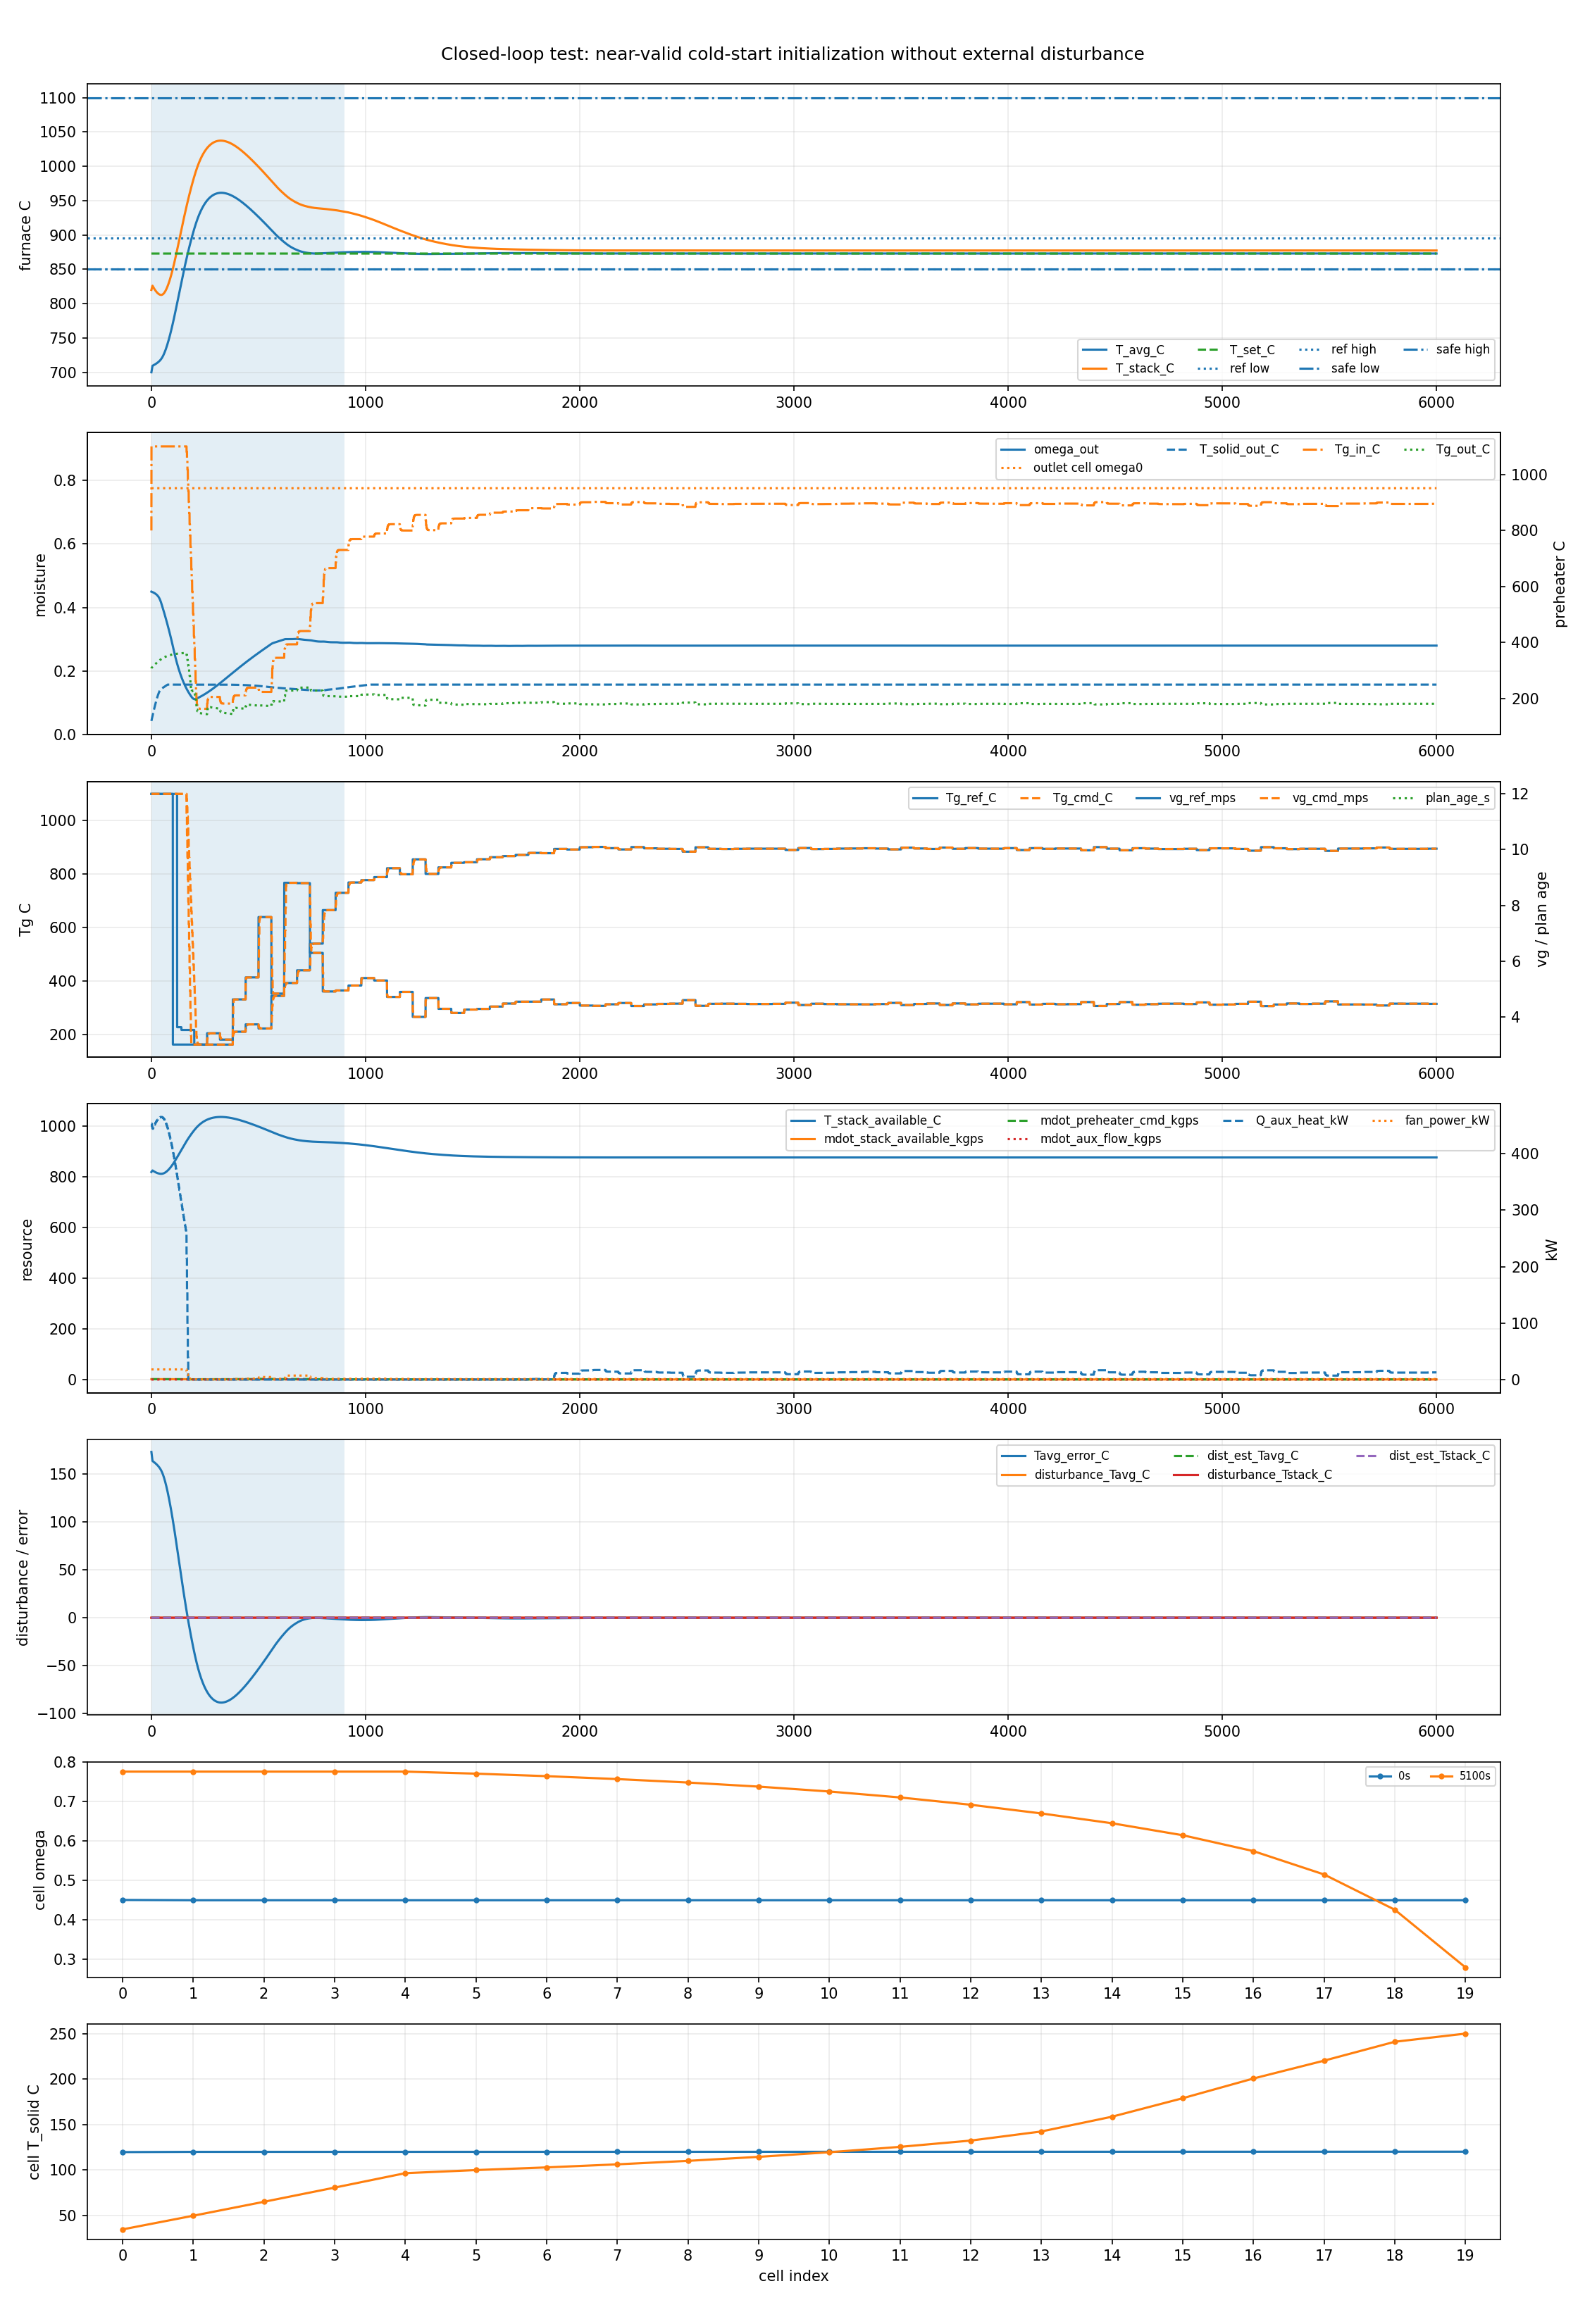
\includegraphics[width=\linewidth]{results/cold_start/overview.png}
\caption{冷启动场景闭环测试结果}
\label{fig:result-cold-start}
\end{figure}

\passthrough{\lstinline!cold_start!} 场景采用较低初始炉温和较高初始出口含水率，用于检验低温初始状态下的恢复能力，结果如图 \ref{fig:result-cold-start} 所示。初始 \(T_{avg}\) 约为 700 $^\circ$C，明显低于合规温度下限；\(\omega_{out}\) 初值约为 0.45，预热炉初始固体温度也处于较低水平。开局阶段执行命令迅速进入高温高风速恢复状态，炉膛温度先快速越过安全线并出现超调，随后逐步回落至参考带附近。

全程 \(T_{avg}\) 最低值为 700.07 $^\circ$C，最高值为 961.51 $^\circ$C，安全带占比为 97.45\%，参考带占比为 90.65\%。由于低温初值属于测试设定，前期低温段用于评价恢复机制；尾段 5100--6000 s 的 \(T_{avg}\) 均值为 873.09 $^\circ$C，MAE 为 0.09 $^\circ$C，峰峰值约 0.11 $^\circ$C，参考带和安全带占比均为 100\%。物料侧尾段 \(\omega_{out}\) 恢复到 0.2801 附近，出口固体温度维持在 250 $^\circ$C，说明低温初始状态没有造成长期偏移。

当前统计文件中 \passthrough{\lstinline!recovery_to_safe_s!} 和 \passthrough{\lstinline!recovery_to_ref_s!} 记录为 5100 s，这是采用连续保持窗口后得到的尾段稳定判据；从图 \ref{fig:result-cold-start} 的时间曲线可见，开局阶段炉温已经迅速越过安全线，随后经历一次超调回落并在后段形成稳定平台。全程 \passthrough{\lstinline!recovery_guard_ratio!} 为 2.73\%，补热能量为 119272.26 kJ，风机能量为 9569.72 kJ；尾段补热能量降至 11138.28 kJ，风机能量为 832.38 kJ。该结果表明 recovery guard 能够处理低温初始状态，尾段闭环精度与稳态保持场景接近，主要工程代价集中在启动恢复阶段。

\subsection{综合分析}\label{subsec:result-overall-analysis}

五个标准场景的共同结果表明，当前控制器在求解可靠性和尾段稳定性上表现一致：所有场景均未出现 operator fallback 和 stale plan，尾段参考带占比均为 100\%，尾段温度波动均较小。其中，稳态保持、临时扰动恢复后和冷启动尾段的 \(T_{avg}\) MAE 均约为 0.1 $^\circ$C，说明模型预测、执行层限速/滞后和重优化机制在无持续偏置条件下能够形成高精度稳态。

扰动响应方面，临时扰动场景验证了 recovery guard 的短时兜底作用；永久扰动场景验证了动态含水率目标的长期适应能力。永久负温度偏置下，尾段 \(\omega_{out}\) 从常规工况的约 0.280 降至约 0.160，说明控制器通过降低入炉等效含水率补偿持续热损失。该行为与第三章给出的动态含水率目标设计相一致，也提示永久性热损失需要关注物料过度干化、辅助补热和风机能耗之间的工程权衡。

资源侧结果显示，多个场景中 \passthrough{\lstinline!aux_resource_required_ratio!} 和 \passthrough{\lstinline!aux_circulation_required_ratio!} 较高，来料阶跃、永久扰动和冷启动场景的全程补热能量均超过 $1.0\times10^5$ kJ。该现象说明当前控制参数更偏向温度安全和出口含水率稳定，经济性仍有进一步优化空间。后续调参可优先检查三类内容：一是自然烟气资源上限与资源 predictor 的标定，二是 \passthrough{\lstinline!r_aux_heat!}、\passthrough{\lstinline!r_fan_power!} 和 \passthrough{\lstinline!r_economic_vg!} 等经济性权重，三是来料阶跃和永久扰动场景下的目标温度带与含水率目标是否需要分工况设定。

从测试判据看，本轮结果支持以下工程判断：控制器能够在无扰动、来料阶跃、临时温度扰动、永久温度扰动和低温初始状态下保持闭环可运行；安全恢复机制能够在低温或不可忽略扰动下给出高强度恢复命令；在扰动结束或系统适应后，闭环可以回到稳定尾段。当前结果也暴露出资源消耗偏高和部分场景稳态温度略低于设定值的问题，这些问题主要属于经济性与稳态偏差调参范畴，后续应结合真实烟气资源能力、辅助补热约束和现场执行器能力继续校核。

\manualdivider

\end{document}
